\documentclass[]{article}



\usepackage{graphicx,forloop,caption,subcaption,float,hyperref,arrayjob,listings,color,booktabs,mathtools}
\usepackage{pdfpages}
\usepackage[margin=1.2in]{geometry}
\usepackage{amsmath}
\usepackage{multirow}
%vhdl code
\definecolor{dkgreen}{rgb}{0,0.6,0}
\definecolor{gray}{rgb}{0.5,0.5,0.5}
\definecolor{mauve}{rgb}{0.58,0,0.82}

\DeclareMathOperator*{\argmin}{\arg\!\min}
\newcommand{\rom}[1]{\uppercase\expandafter{\romannumeral#1}}

\lstset{frame=tb,
  language=VHDL,
  aboveskip=3mm,
  belowskip=3mm,
  showstringspaces=false,
  columns=flexible,
  basicstyle={\small\ttfamily},
  numbers=none,
  numberstyle=\tiny\color{gray},
  keywordstyle=\color{blue},
  commentstyle=\color{dkgreen},
  stringstyle=\color{mauve},
  breaklines=true,
  breakatwhitespace=true
  tabsize=3
}

%matlab code
\lstset{frame=tb,
  language=Matlab,
  aboveskip=3mm,
  belowskip=3mm,
  showstringspaces=false,
  columns=flexible,
  basicstyle={\small\ttfamily},
  numbers=none,
  numberstyle=\tiny\color{gray},
  keywordstyle=\color{blue},
  commentstyle=\color{dkgreen},
  stringstyle=\color{mauve},
  breaklines=true,
  breakatwhitespace=true
  tabsize=3
}


% Title Page
\title{UCLA\\EE230B\\Digital Communication Design Project\\Step 2 Report}
\author{Alican Salor 404271991 \\  \href{mailto:alicansalor@ucla.edu}{alicansalor@ucla.edu} \\ \\
Darren Reis 804359840 \\
\href{mailto:darrer.r.reis@gmail.com}{darren.r.reis@gmail.com} }


\begin{document}
\maketitle

\newpage
\tableofcontents

\newpage


\section{System Setup}
\label{sec:setup}
To handle the noncoherent error introduced into the system, feedback loops(costas and decision directed) were installed.  As from before, the $\delta\phi$ block represents a block that introduces phase or frequency offset on the carrier.  To combat this, the error is estimated and then fed into a feedback loop filter to track it out. \\

Both of these setups are based on the same control theory fundamentals and thus have similar feedback loop components. In control theory when there is steady state error in the open loop system, feedback, or `closing the loop' can track out the error.  From the plots in Step 2, we realize our situation is just this case of steady state error.  Depending on the order of the system, this error can become unbounded and damning.  Feedback can track or bound this error by `closing the loop' if the open loop system Type is 0.  \footnote{Recall, a system is of Type N when there N poles at the s-plane origin.}  Here, the steady state error can be held to a certain level by introducing integration in the feedback line of the loop.  For us, this is true when we talk about phase error: we can send a step input phase error into a Voltage Controlled Oscillator and watch the error converge to a constant level. 
\begin{align}
\label{eq:vco}
\phi_{\text{out}} &= \int \! k_{VCO}V_{in} \mathrm{d}t
\end{align}
A VCO is a device with output oscillation which is varied by the voltage level of the input.  The transfer function, relating the input to the output, for this block is shown in Equation~\ref{eq:vco}. The integral action can eliminate phase error, as we see in Figure~\ref{fig:BLAH}.  To implement a VCO in simulation, a phase accumulator does the integration   action and then, to keep the result in the correct domain, the result is put through a modulo $2\pi$ block.   
When the plant is of higher Type than 0, as with a frequency offset, the steady state error can grow unbounded.  To deal with this scenario, another block is inserted in the feedback line.  An additional integrator increases the order of the closed loop system to allow bounding of higher type systems.  Notice in Figure~\ref{fig:costas}, the loop filter is Proportional-Integral.  With two integrators in the feedback path, Type 1 systems, or those with ramp inputs, can be bounded to a constant steady state error level.  Because frequency can be thought of as first order phase [\ref{eq:phaseFreq}], we track out the frequency error.\\
\begin{align}
\label{eq:phaseFreq}
\phi &= \int \! 2\pi f \mathrm{d}t 
\end{align}


Furthermore as it can be seen in the simultion files, a different approach of coding is taken compared to the previous simulations. Note that unlike in previous simulations of the system, this analysis required sample-wise operations instead of signal-wise operations. That is, to maintain causality, the samples were analyzed one by one so that future samples could not influence present values.\\

In the following sections the two setups for error recovery is given and their error metrics are examined.


\newpage

\subsection{System with Costas Loop}
This error recovery is accomplished first via a Costas loop, as in Figure~\ref{fig:costas}. 

\begin{figure}[H]
\centering
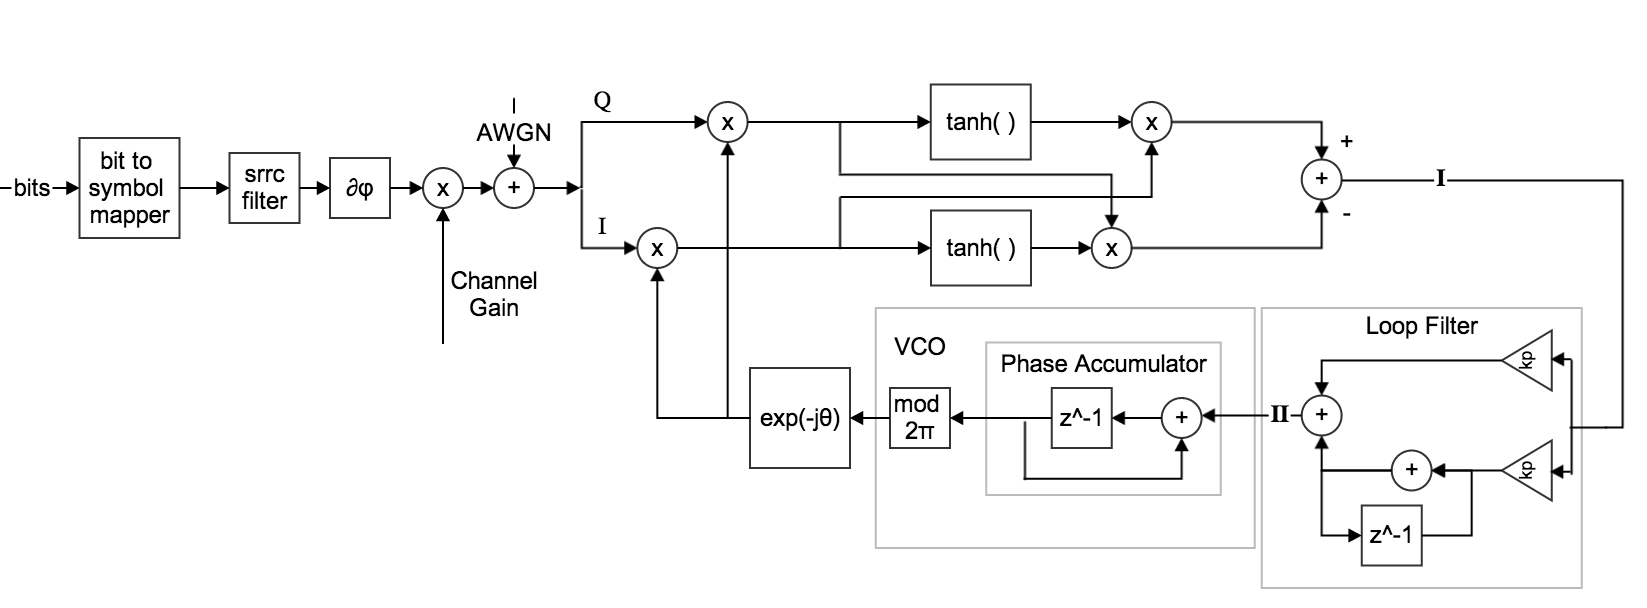
\includegraphics[width=\textwidth]{costas.png}
\caption{Diagram of the Costas loop used to handle error\label{fig:costas}}
\end{figure}

The phase and frequency offset error, under QPSK, can be handled by the Costas loop given above. The technique first creates an estimate of the phase error by creating a metric for it.  The error is then sent through a closed feedback loop.  This structure can track out the zero order (phase offset) and first order (carrier offset) phase errors as it containes two integrators. 

In a Costas loop, the I and Q component of the received signal are both sent through a $\tanh\left(\cdot\right)$ block in order to discern their sign.  This works because for $k>>1$, $\text{sign}\left(x\right) \approx \tanh \left(x\right)$.  These $\pm1$ are multiplied by the opposite component signal.  The I component is then subtracted from the Q component, creating a phase error metric [\ref{eq:costas}].  This is labeled in Figure~\ref{fig:costas} as \rom{1}. 

Now with an error metric, we have the following input 

\begin{align}
  \label{eq:costas}
  S_{\mathcal{l}} &= \left[I\left(t\right)\sin\left(\phi_e\right)+Q\left(t\right)\cos\left(\phi_e\right)\right]\text{sign}\left(I\left(t\right)\cos\left(\phi_e\right)- Q\left(t\right)\sin\left(\phi_e\right)\right)\nonumber \\
  &\qquad {} - \left[I\left(t\right)\cos\left(\phi_e\right)-Q\left(t\right)\sin\left(\phi_e\right)\right]\text{sign}\left(I\left(t\right)\sin\left(\phi_e\right)+Q\left(t\right)\cos\left(\phi_e\right)\right)
  \end{align}


to run into a loop filter and then the VCO. Finally the output of the VCO is used to correct the received signal's phase error as seen in the system setup in Figure~\ref{fig:costas}

\newpage
\subsection{System with Decision Directed Recovery Loop}
Another approach to recover the phase and carrier offset is using the Decision Directed Recovery Loop. The setup is as shown in the figure below:
\begin{figure}[H]
\centering
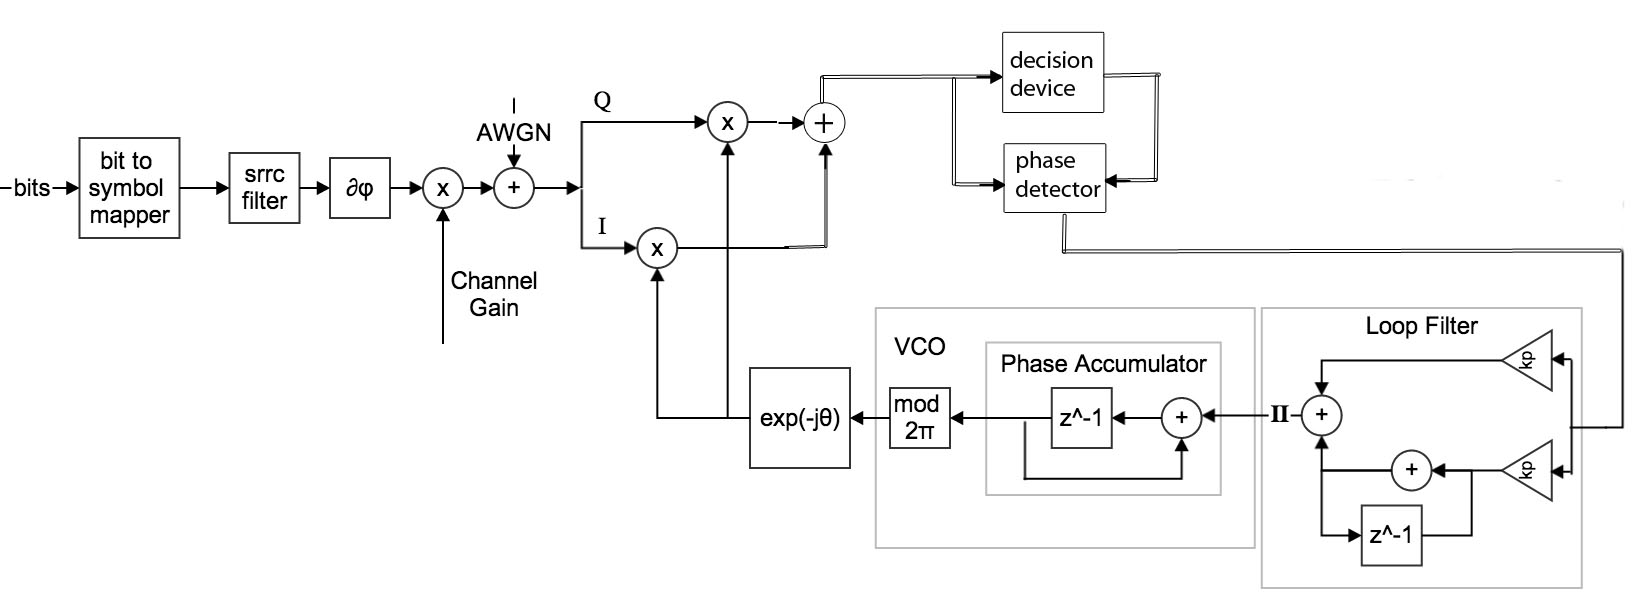
\includegraphics[width=\textwidth]{ddr_diagram.jpg}
\caption{Diagram of the Decision Directed Recovery loop used to handle error\label{fig:ddr}}
\end{figure}

Again this system can handle both phase and frequency offset errors (under QPSK). Similar to the Costas Loop, the phase error is estimated and sent through a closed feedback loop, thus tracking and recovering the error. The system containes two integrators, thus as mention before, zero order (phase offset) and first order (carrier offset) phase errors can be tracked out. 

In the Decision Directed Recovery Loop, differently from the Costas Loop, the output of the decision block is used to obtain an error metric. The sampled received signal and the output of the decision block is passed through a phase detector which has the following function:\\

$\hat{\phi} = sin^{-1}\left(\frac{y(t)\hat{x}^*}{|y(t)||\hat{x(t)}}\right)  $\\

Now that the system has an error metric, it is passed through a loop filter and then a VCO which is then multiplied with the received signal in order to correct the phase/frequency offset as shown in the Figure~\ref{fig:ddr}




\newpage
\section{Step 3 Results}
\subsection{QPSK with Costas Loop}

\subsubsection{S-Curve of Phase Detector}
\begin{figure}[H]
\centering
\hspace*{-2cm}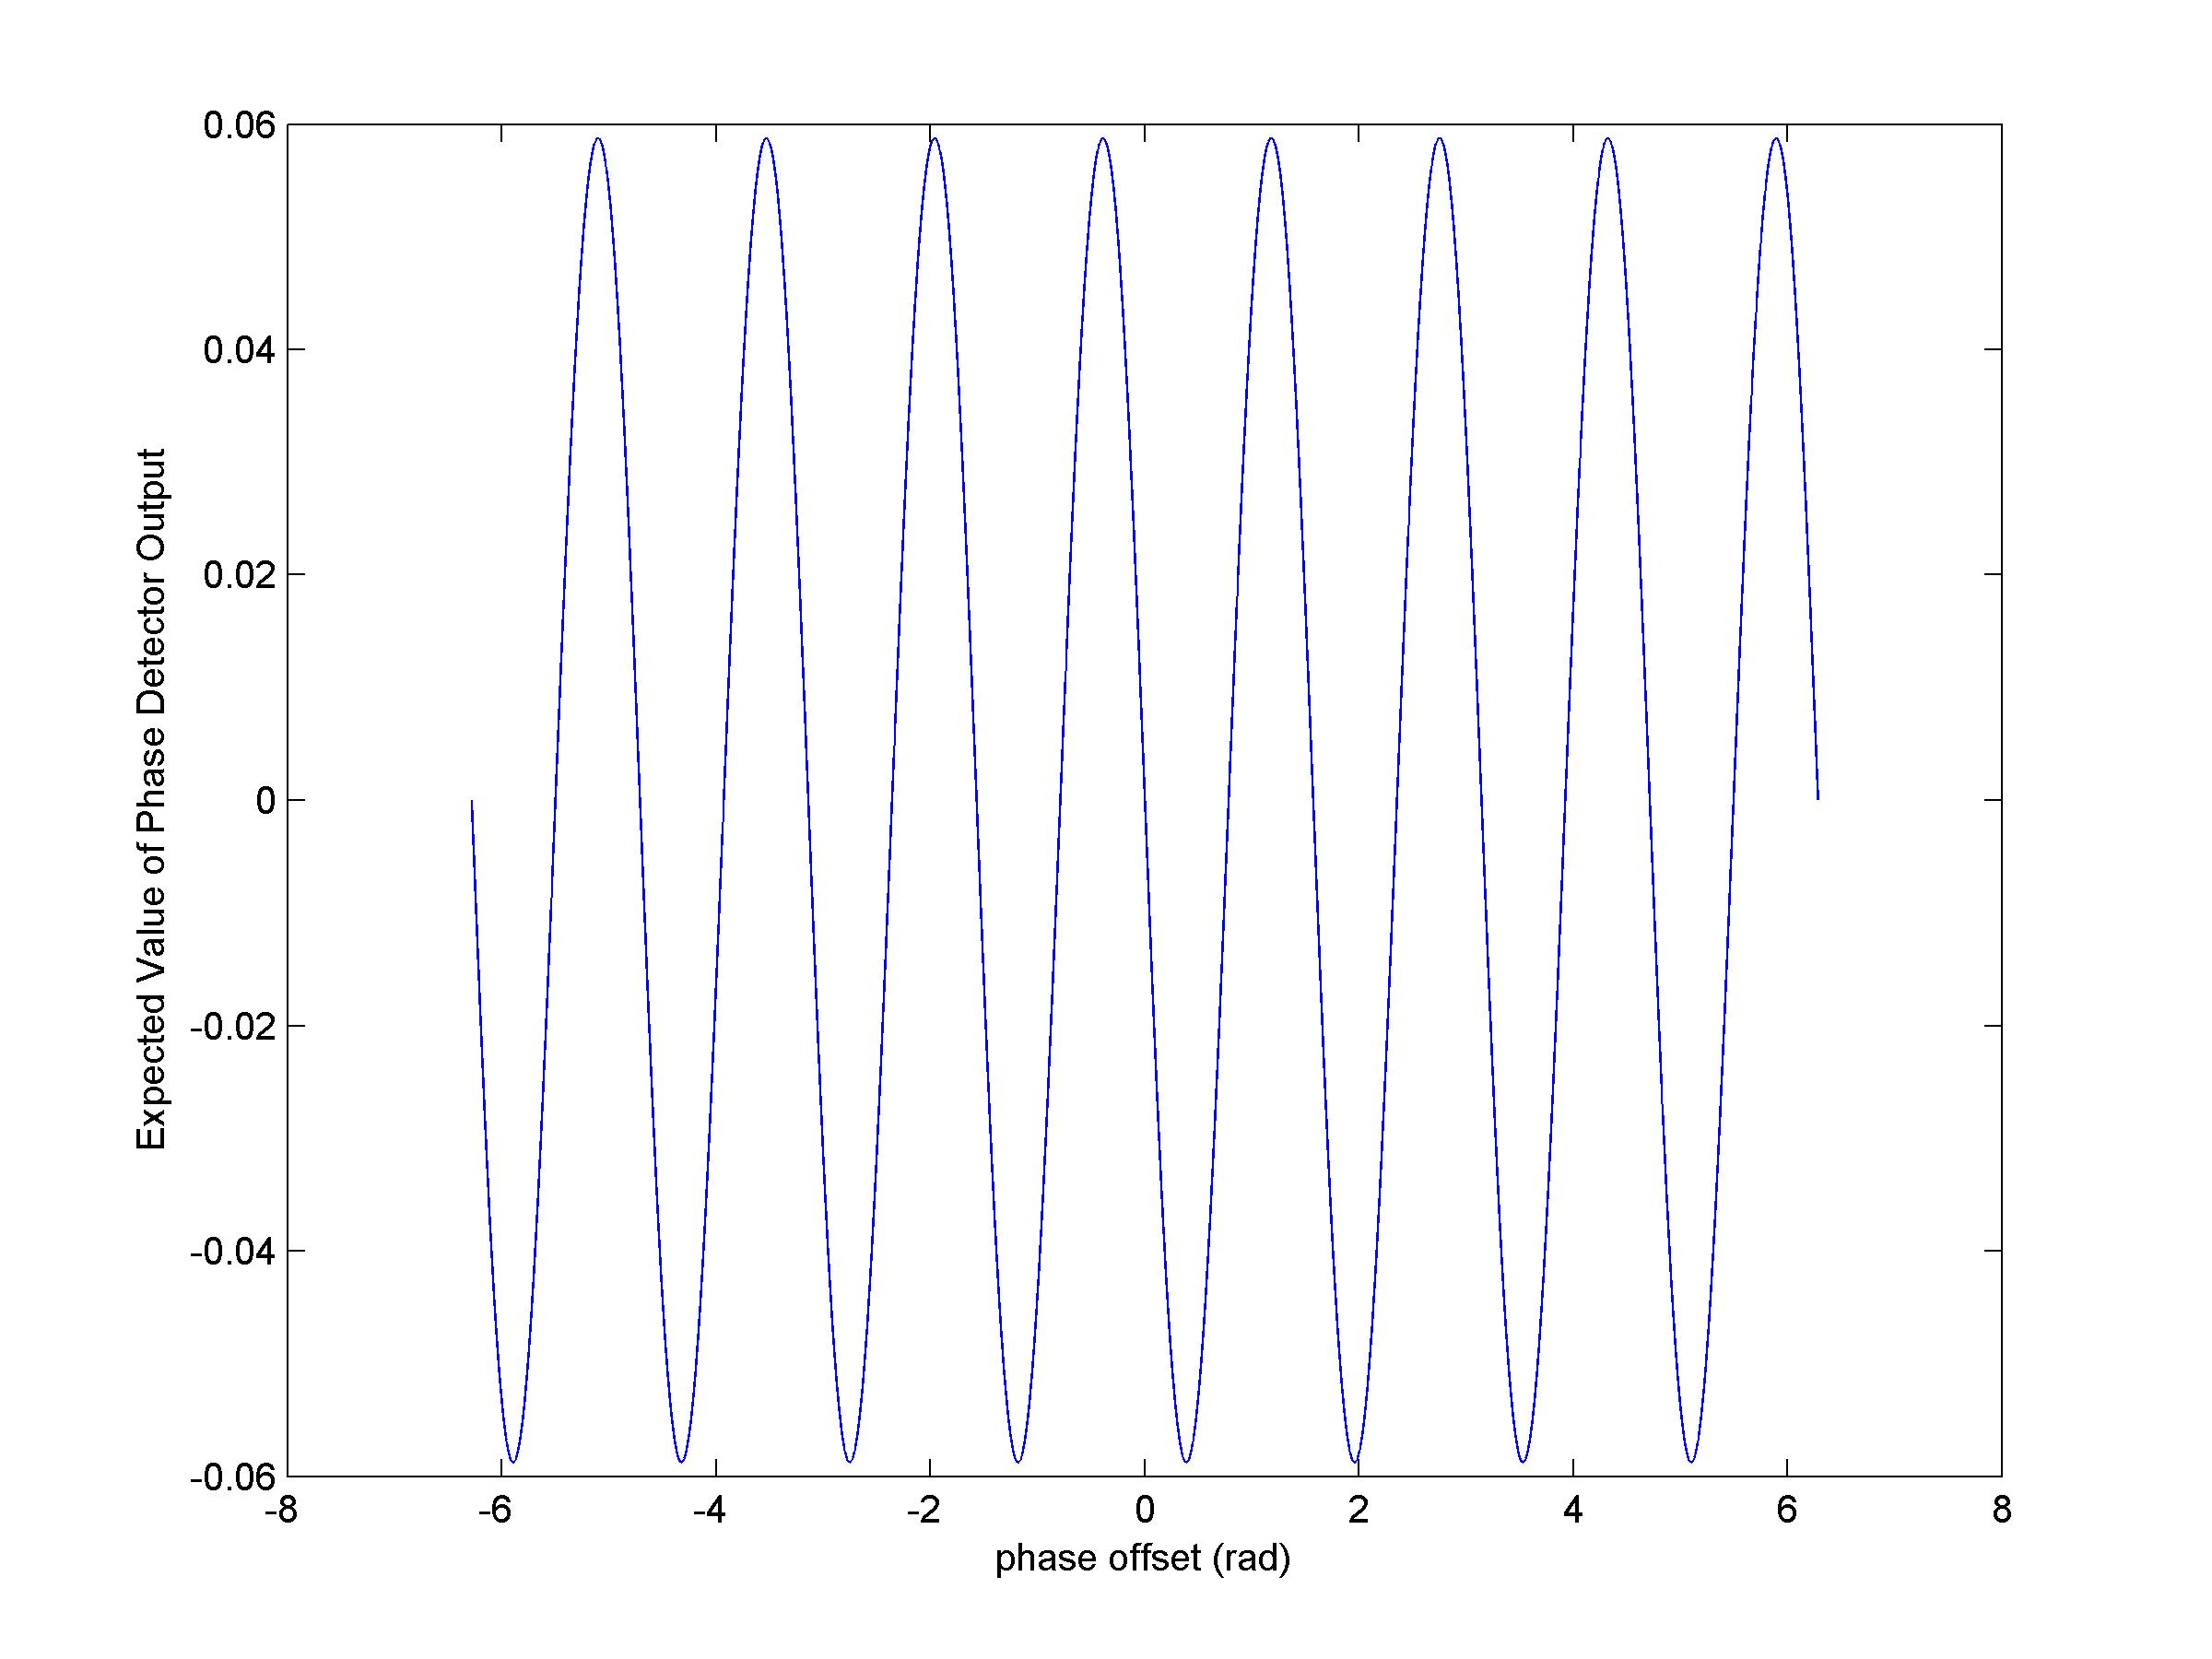
\includegraphics[width=0.7\textwidth]{qpScurvepo_costas.jpg}
\caption{S-curve of the phase detector used in Costas Loop}
\end{figure}
\subsubsection{S-Curve of Carrier Detector}
\begin{figure}[H]
\centering
\hspace*{-2cm}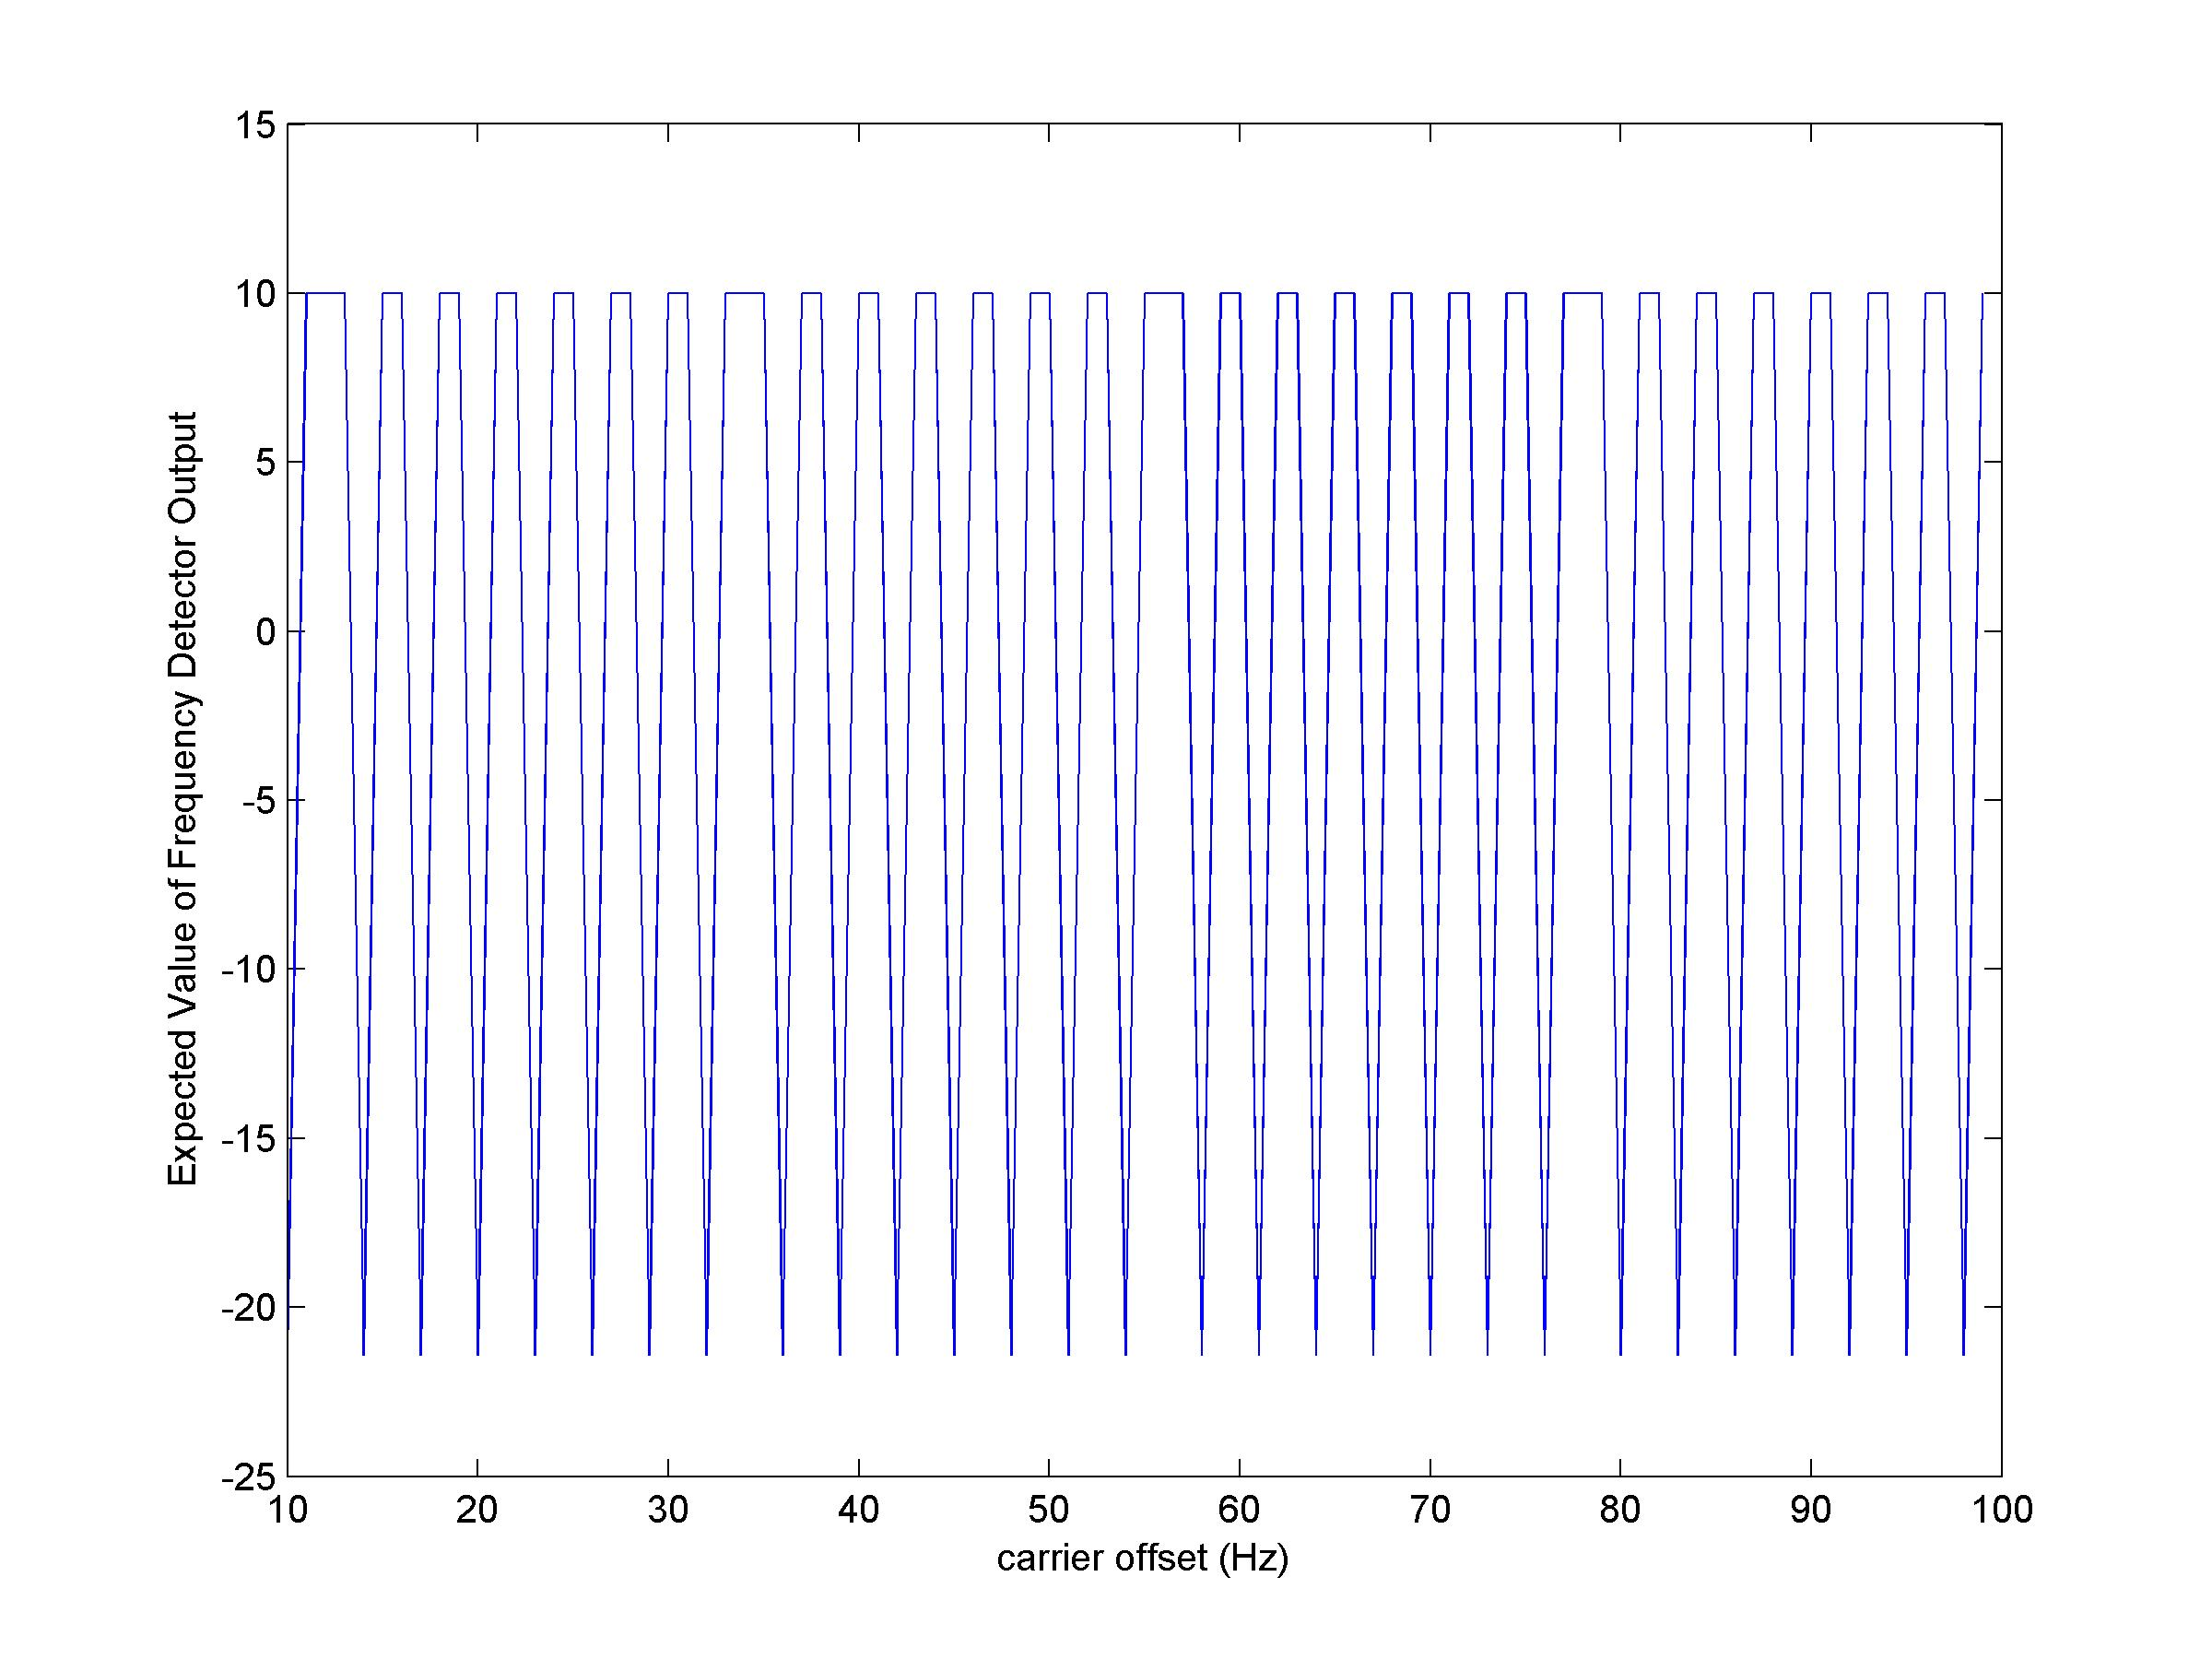
\includegraphics[width=0.7\textwidth]{qpScurvefo.jpg}
\caption{S-curve of the carrier detector used in Costas Loop}
\end{figure}
\subsubsection{Transience of Phase Recovery}
\begin{figure}[H]
\centering
\hspace*{-2cm}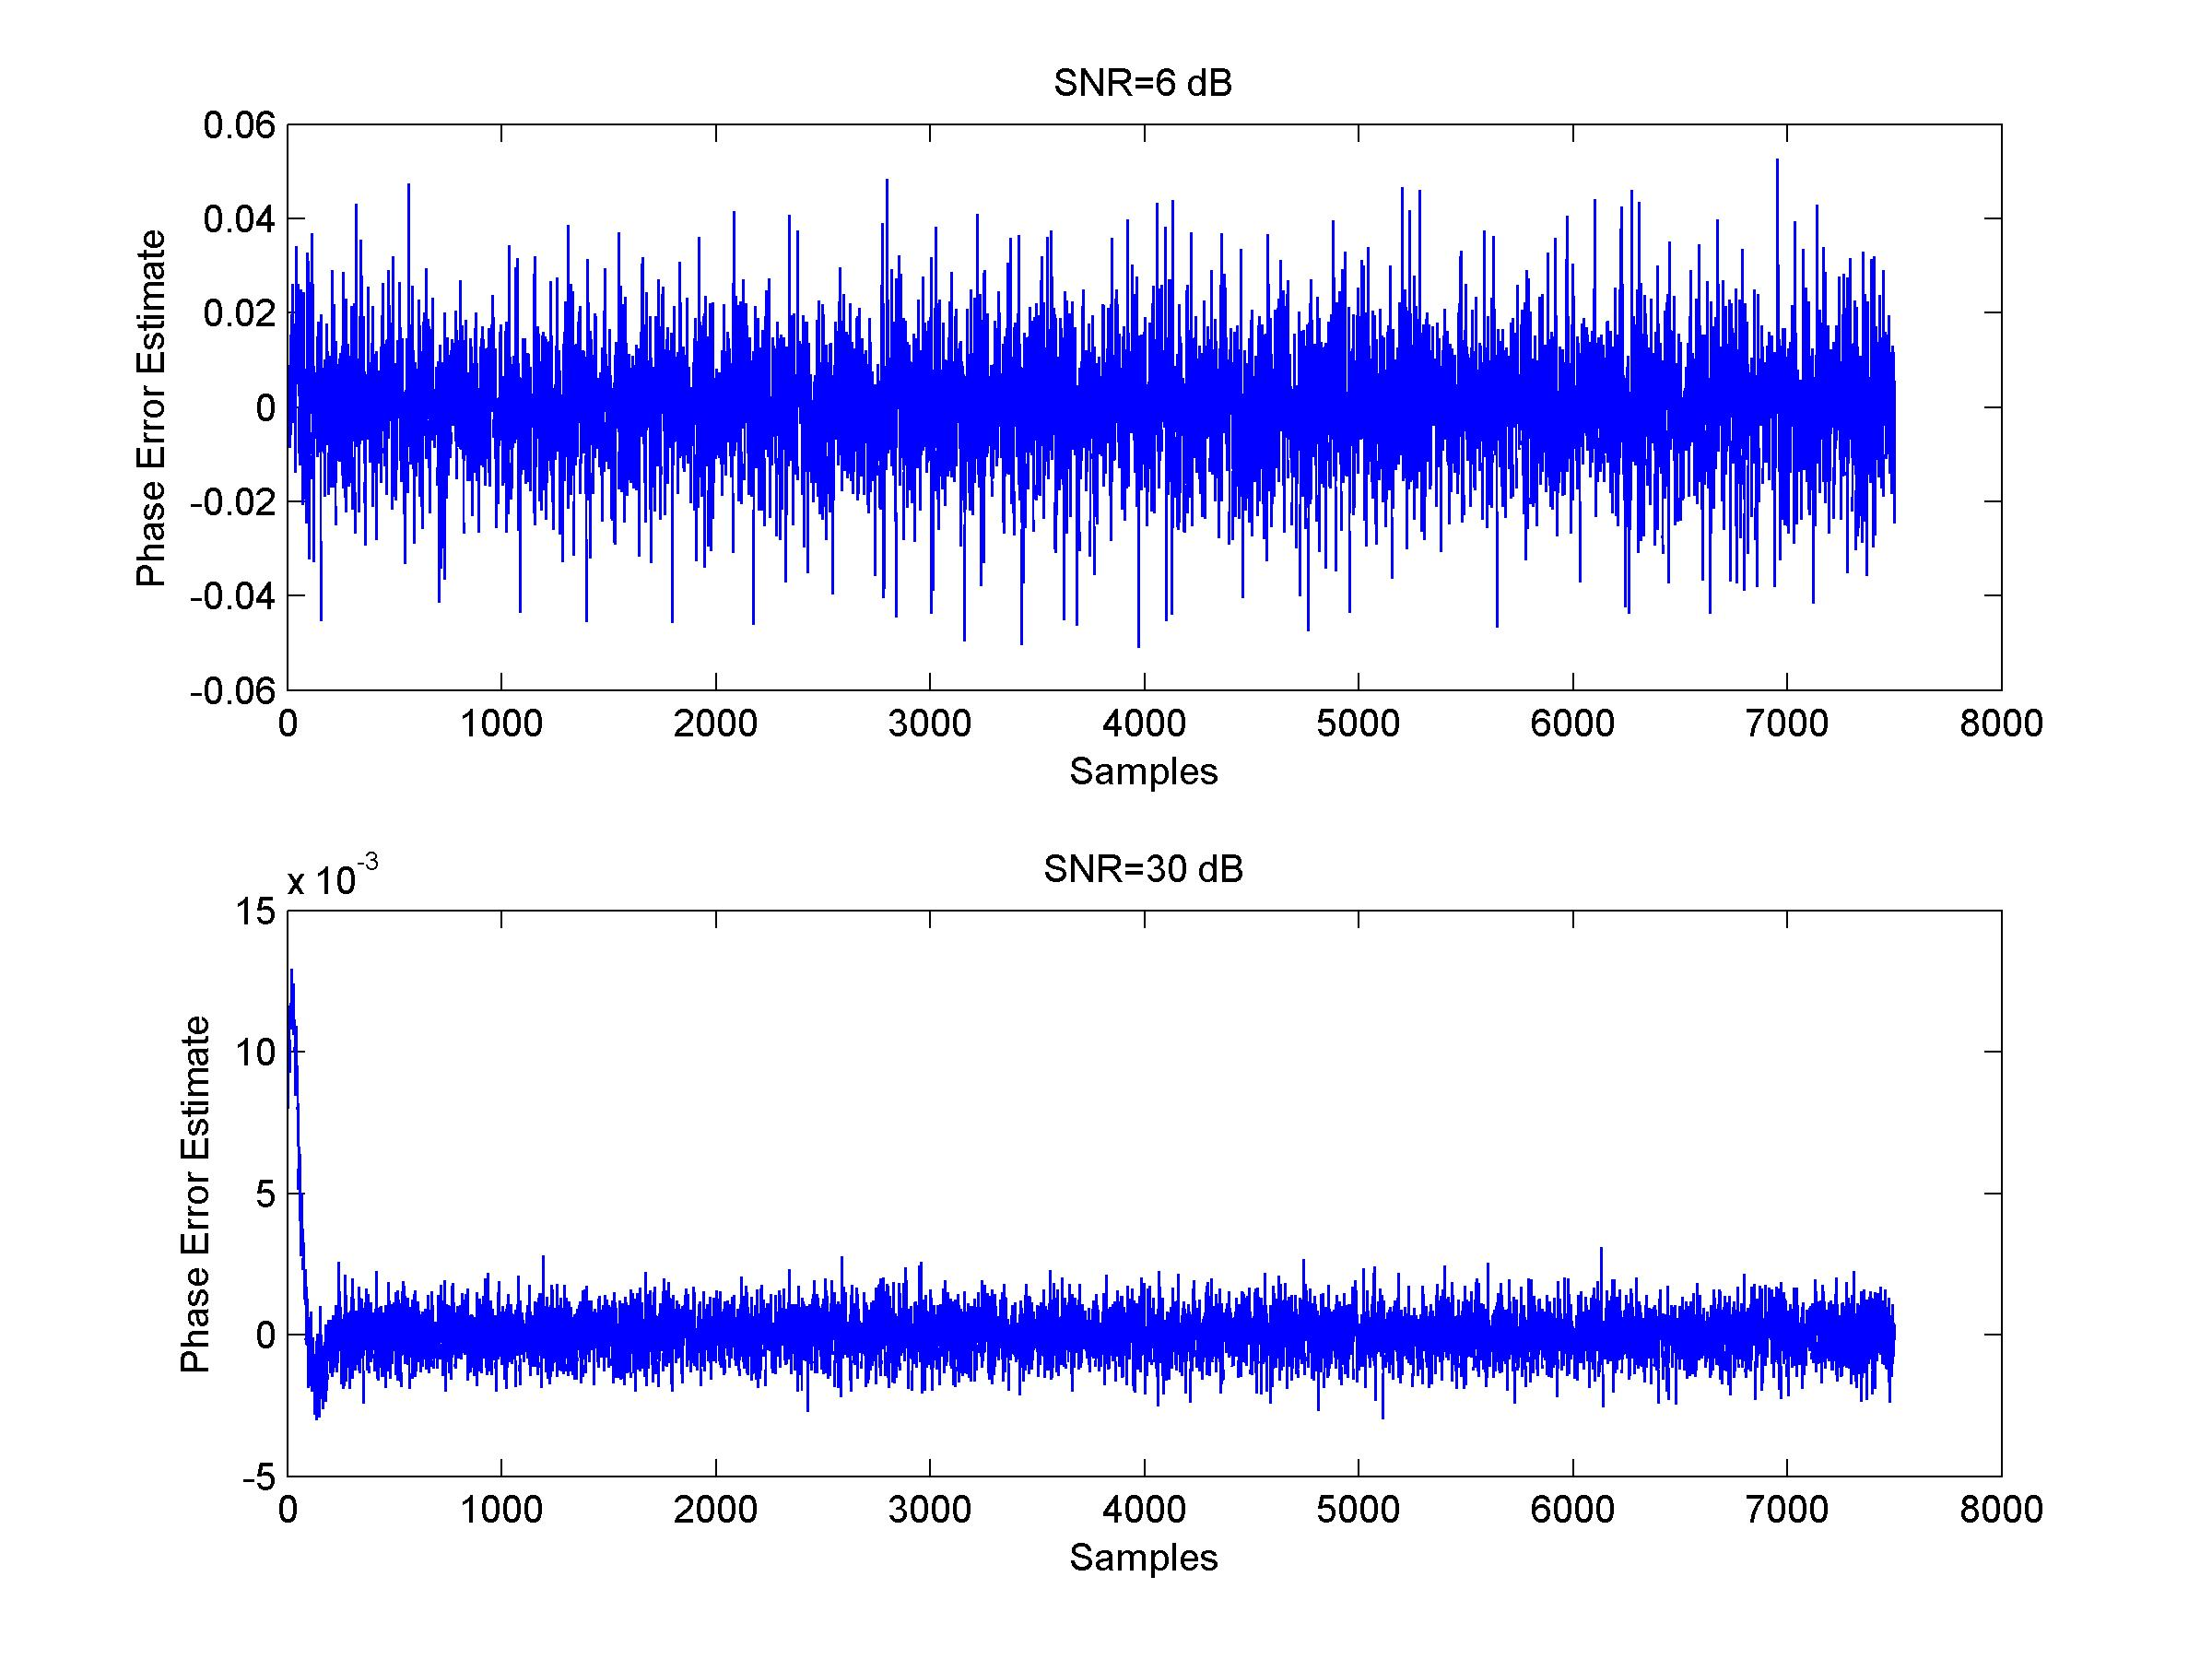
\includegraphics[width=0.7\textwidth]{qpLoopFilterpo_costas1.jpg}
\caption{The loop filter output of the Costas Loop for an input signal with 30 degrees phase offset}
\end{figure}

\subsubsection{Transience of Carrier Recovery}
\begin{figure}[H]
\centering
\hspace*{-2cm}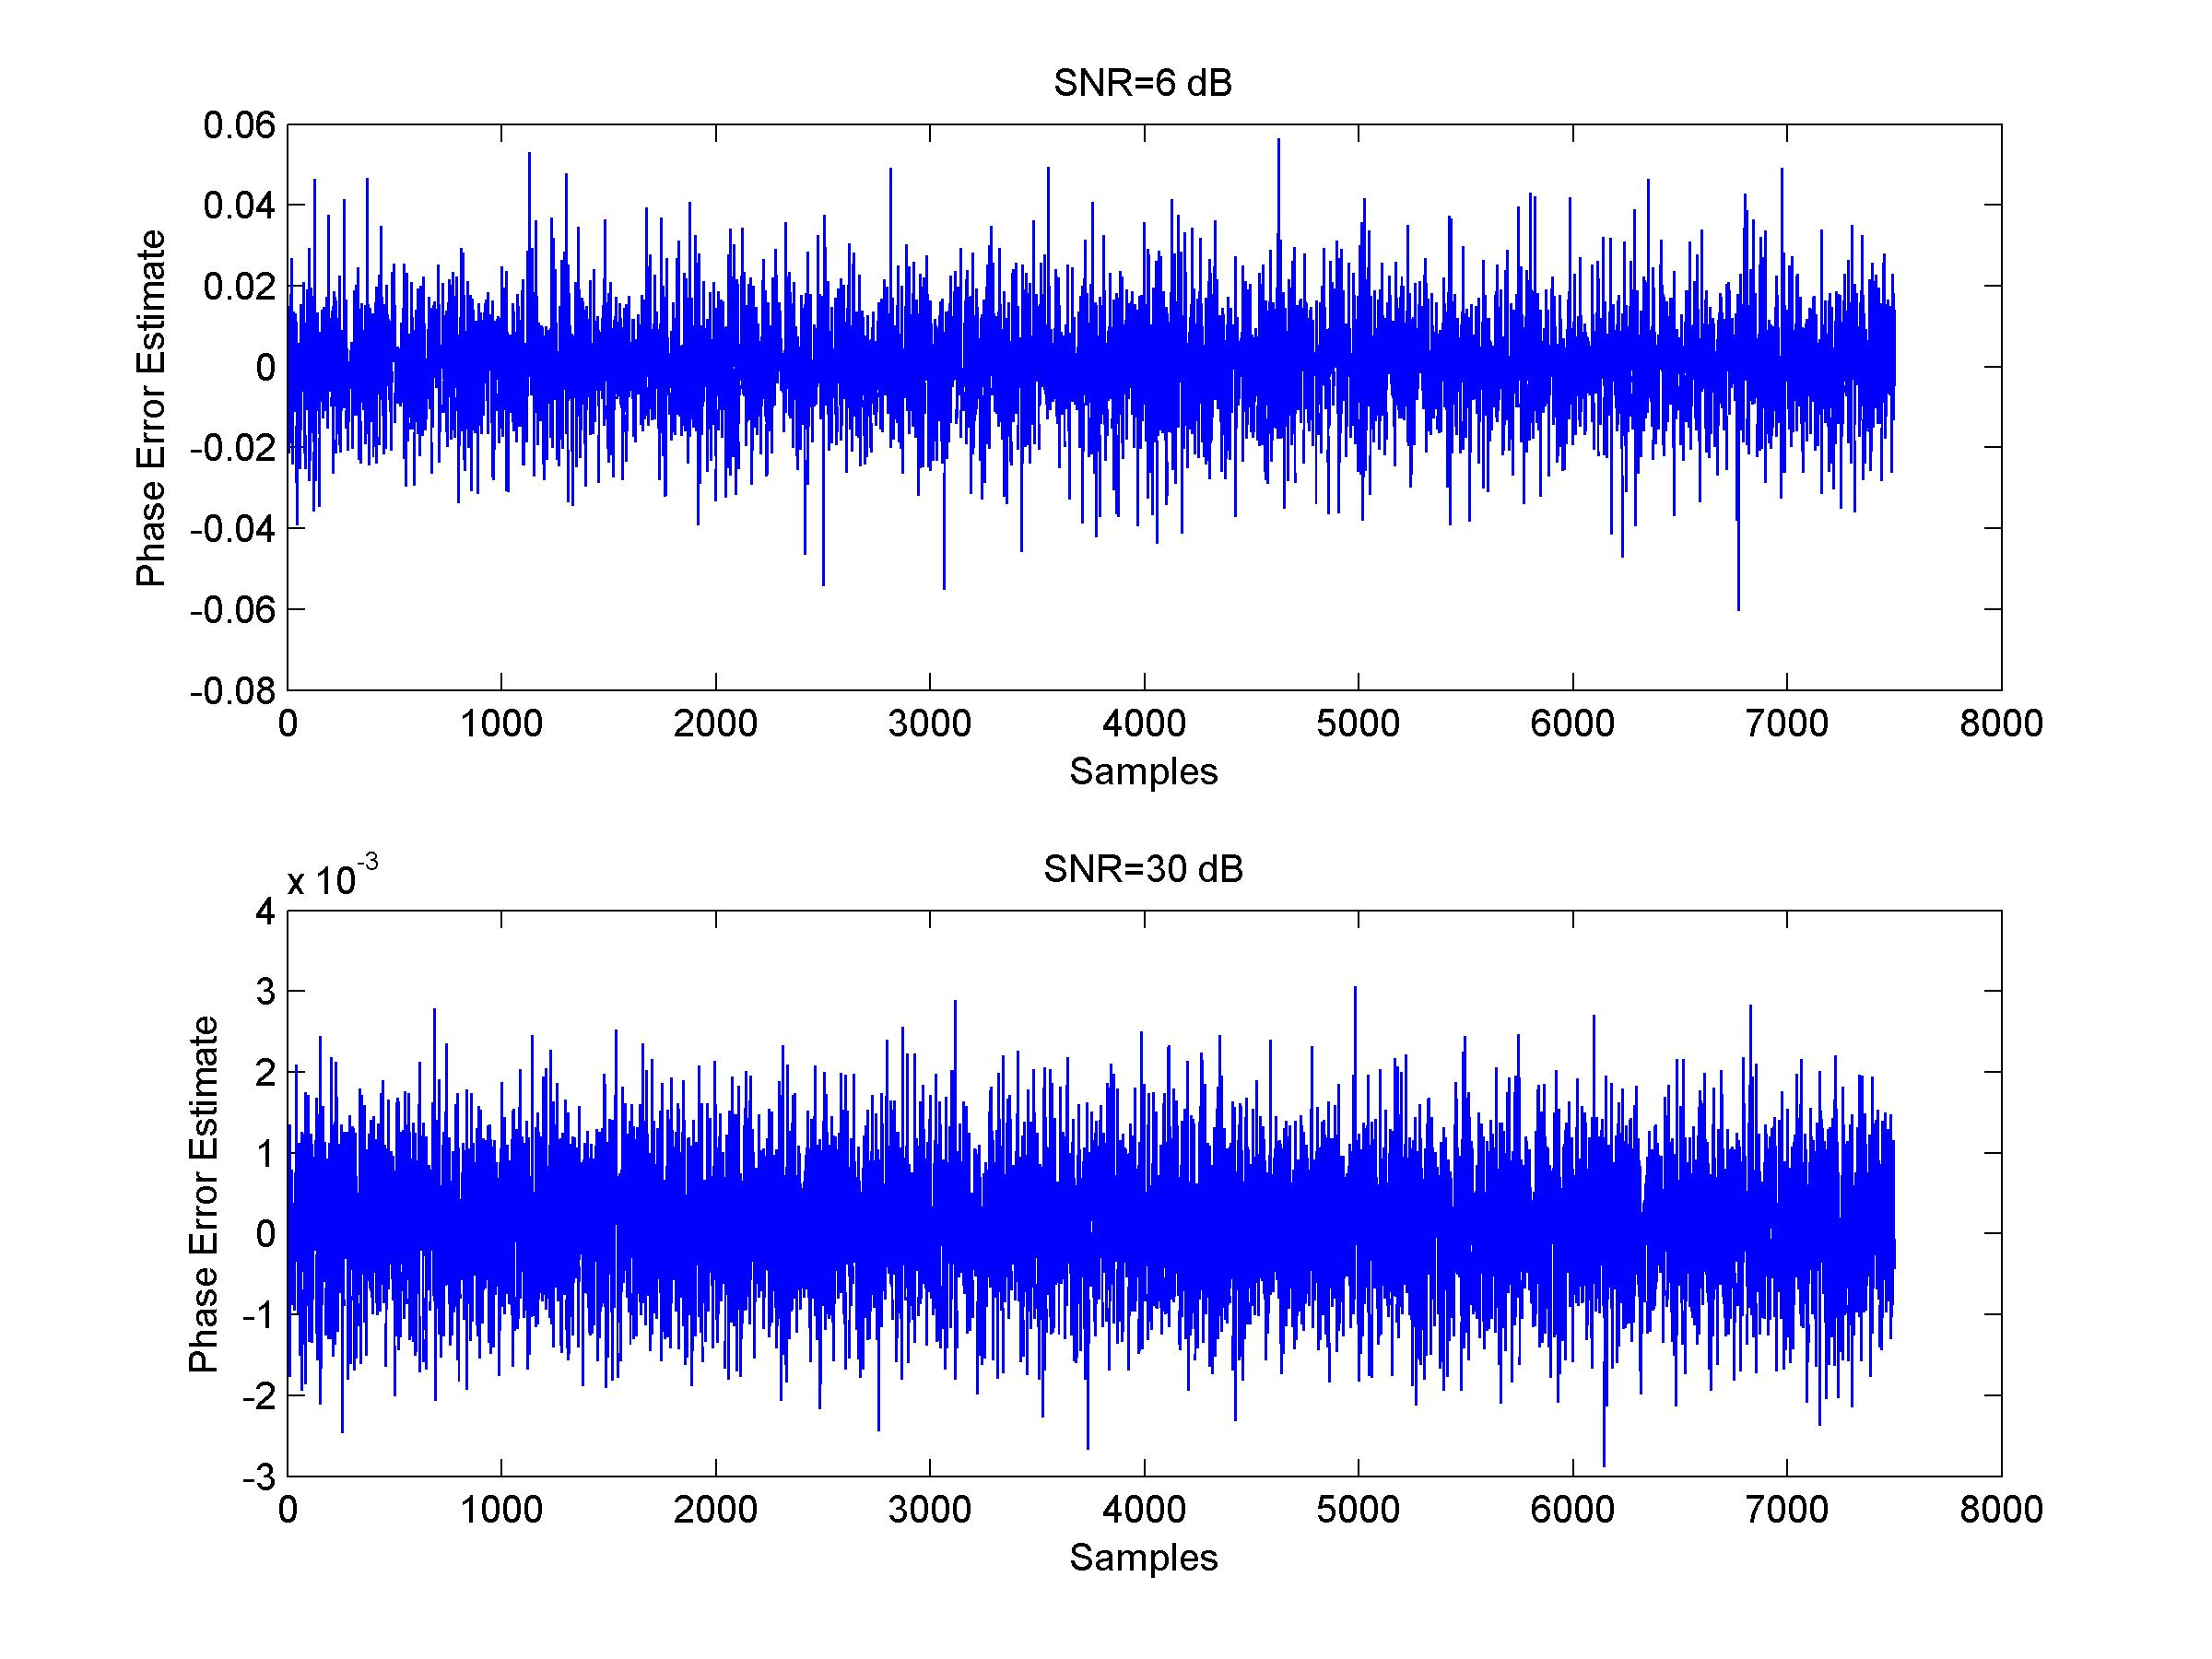
\includegraphics[width=0.7\textwidth]{qpLoopFilterfo_costas1.jpg}
\caption{The loop filter output of the Costas Loop for an input signal with 1ppm frequency offset}
\end{figure}

\begin{figure}[H]
\centering
\hspace*{-2cm}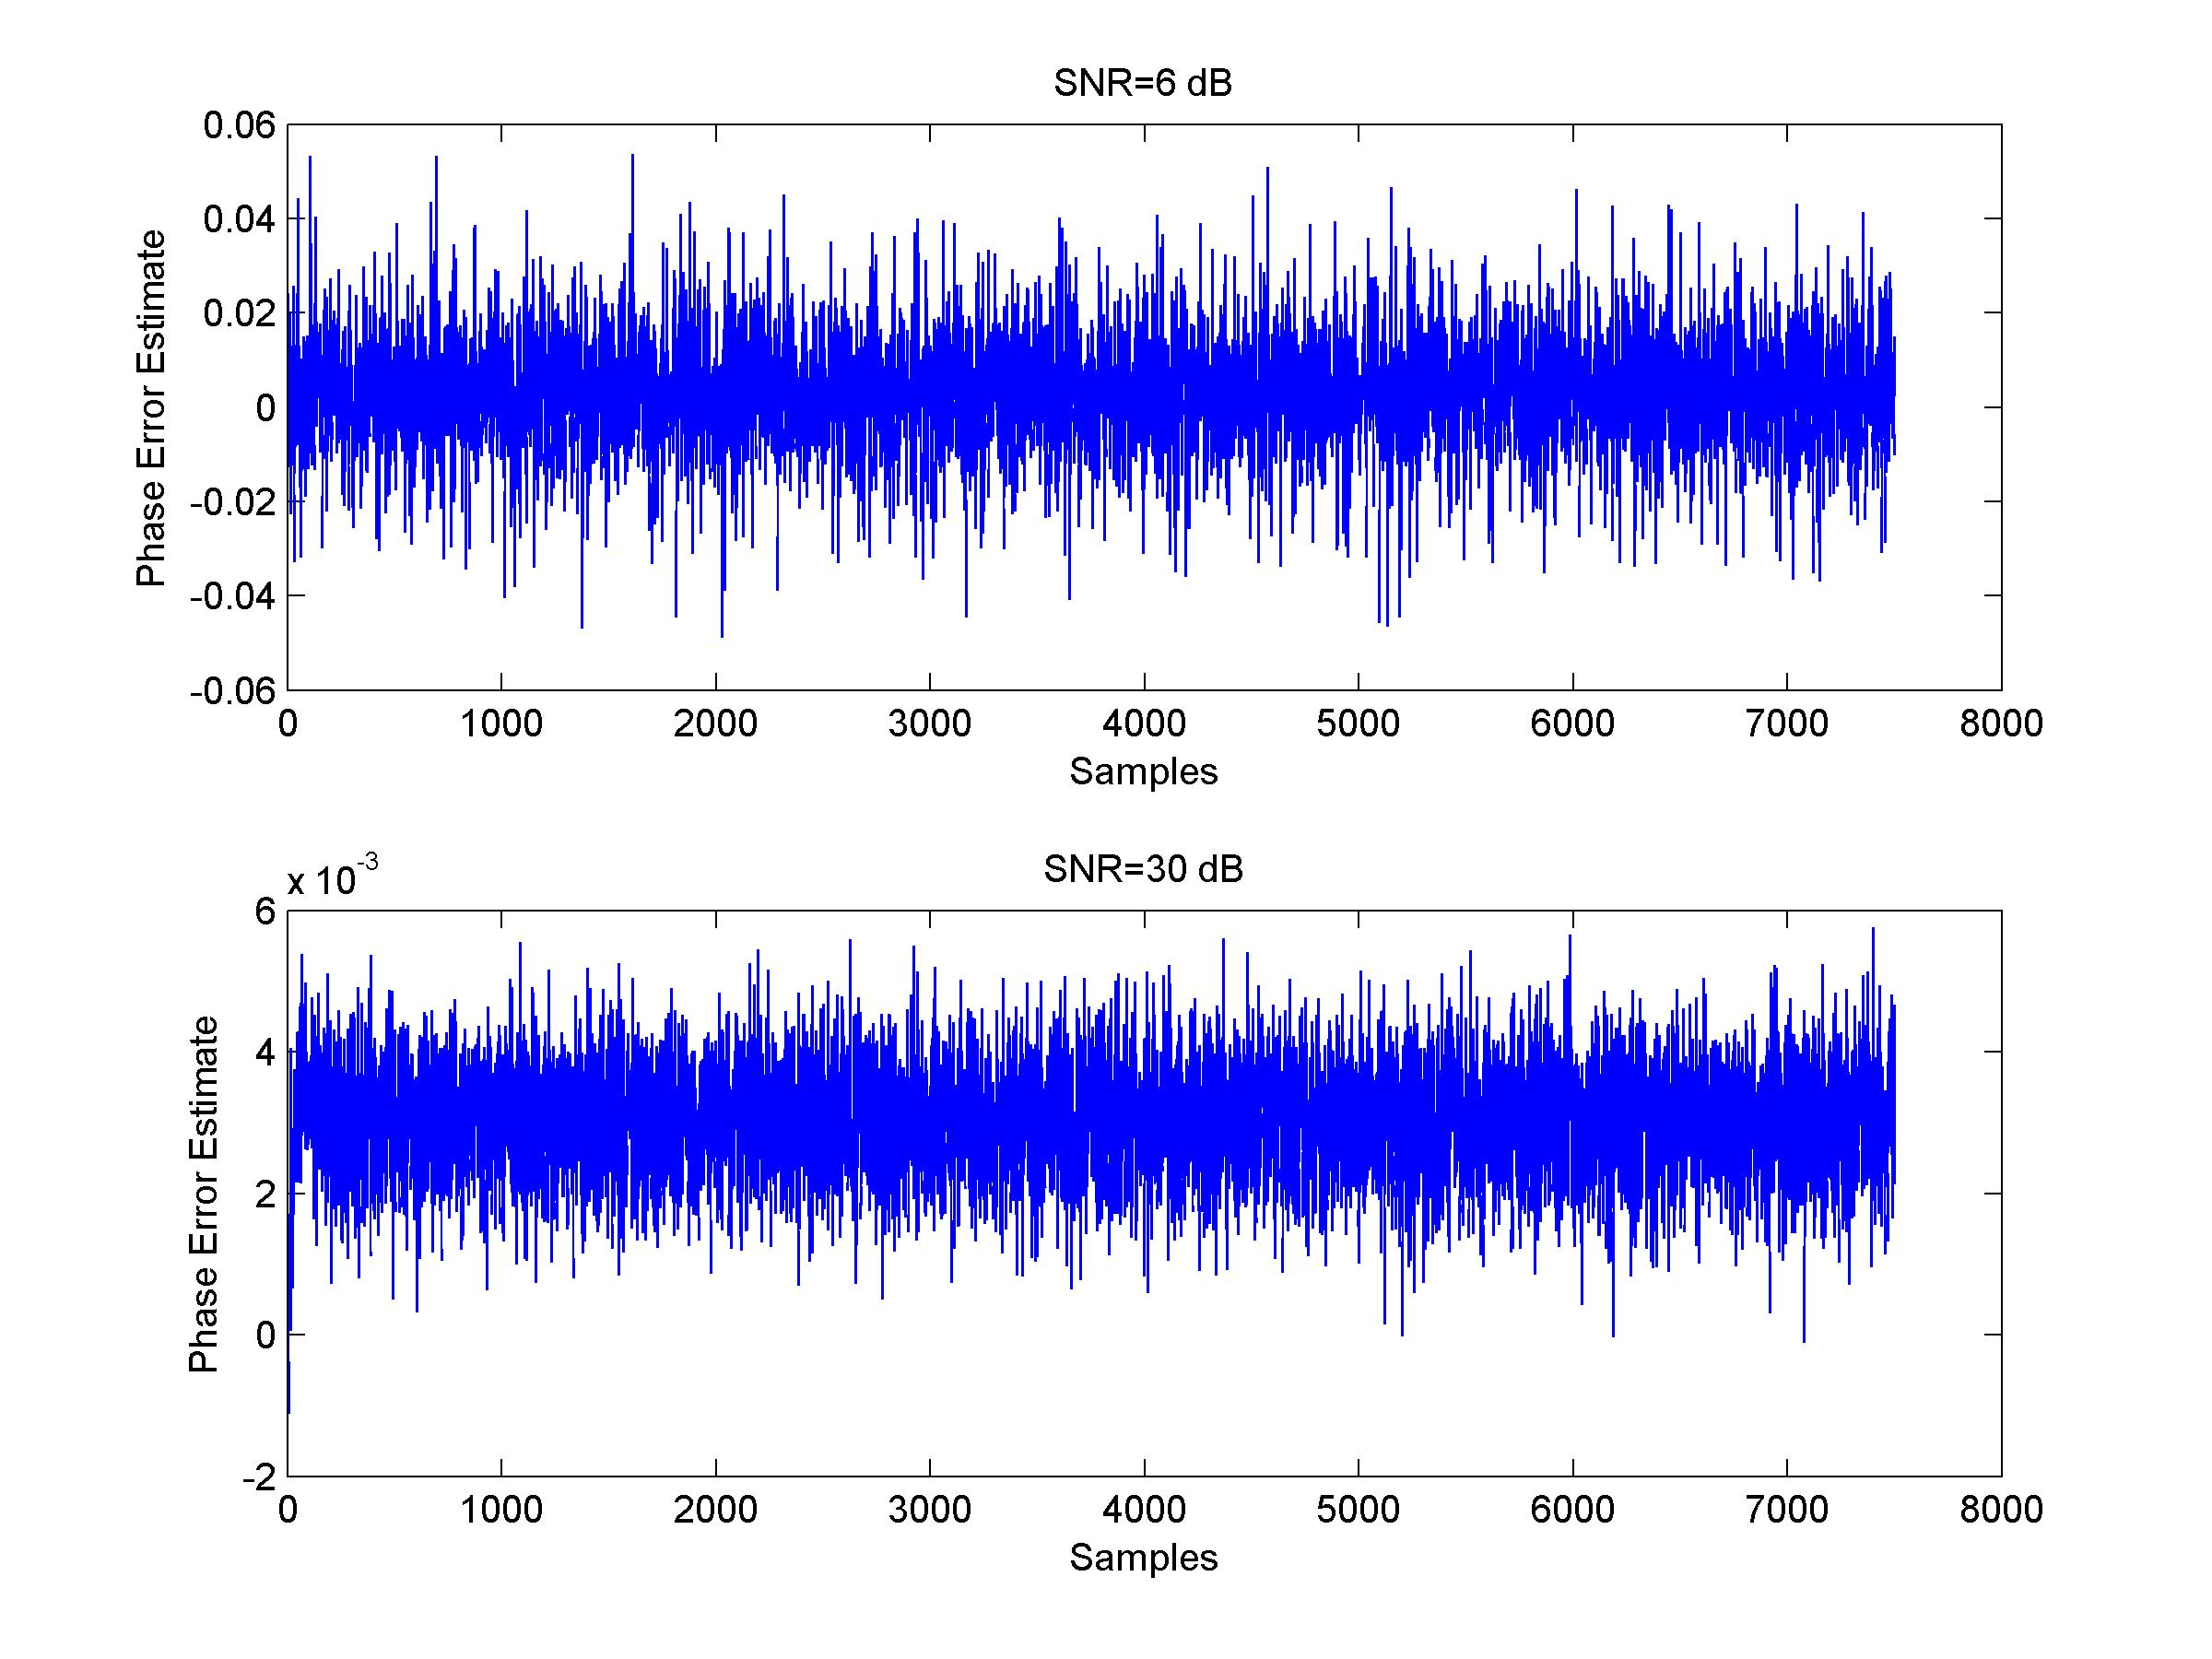
\includegraphics[width=0.7\textwidth]{qpLoopFilterfo_costas2.jpg}
\caption{The loop filter output of the Costas Loop for an input signal with 30ppm frequency offset}
\end{figure}
\subsubsection{Constellation Plots  for Phase Recovery}
\begin{figure}[H]
\centering
\hspace*{-2cm}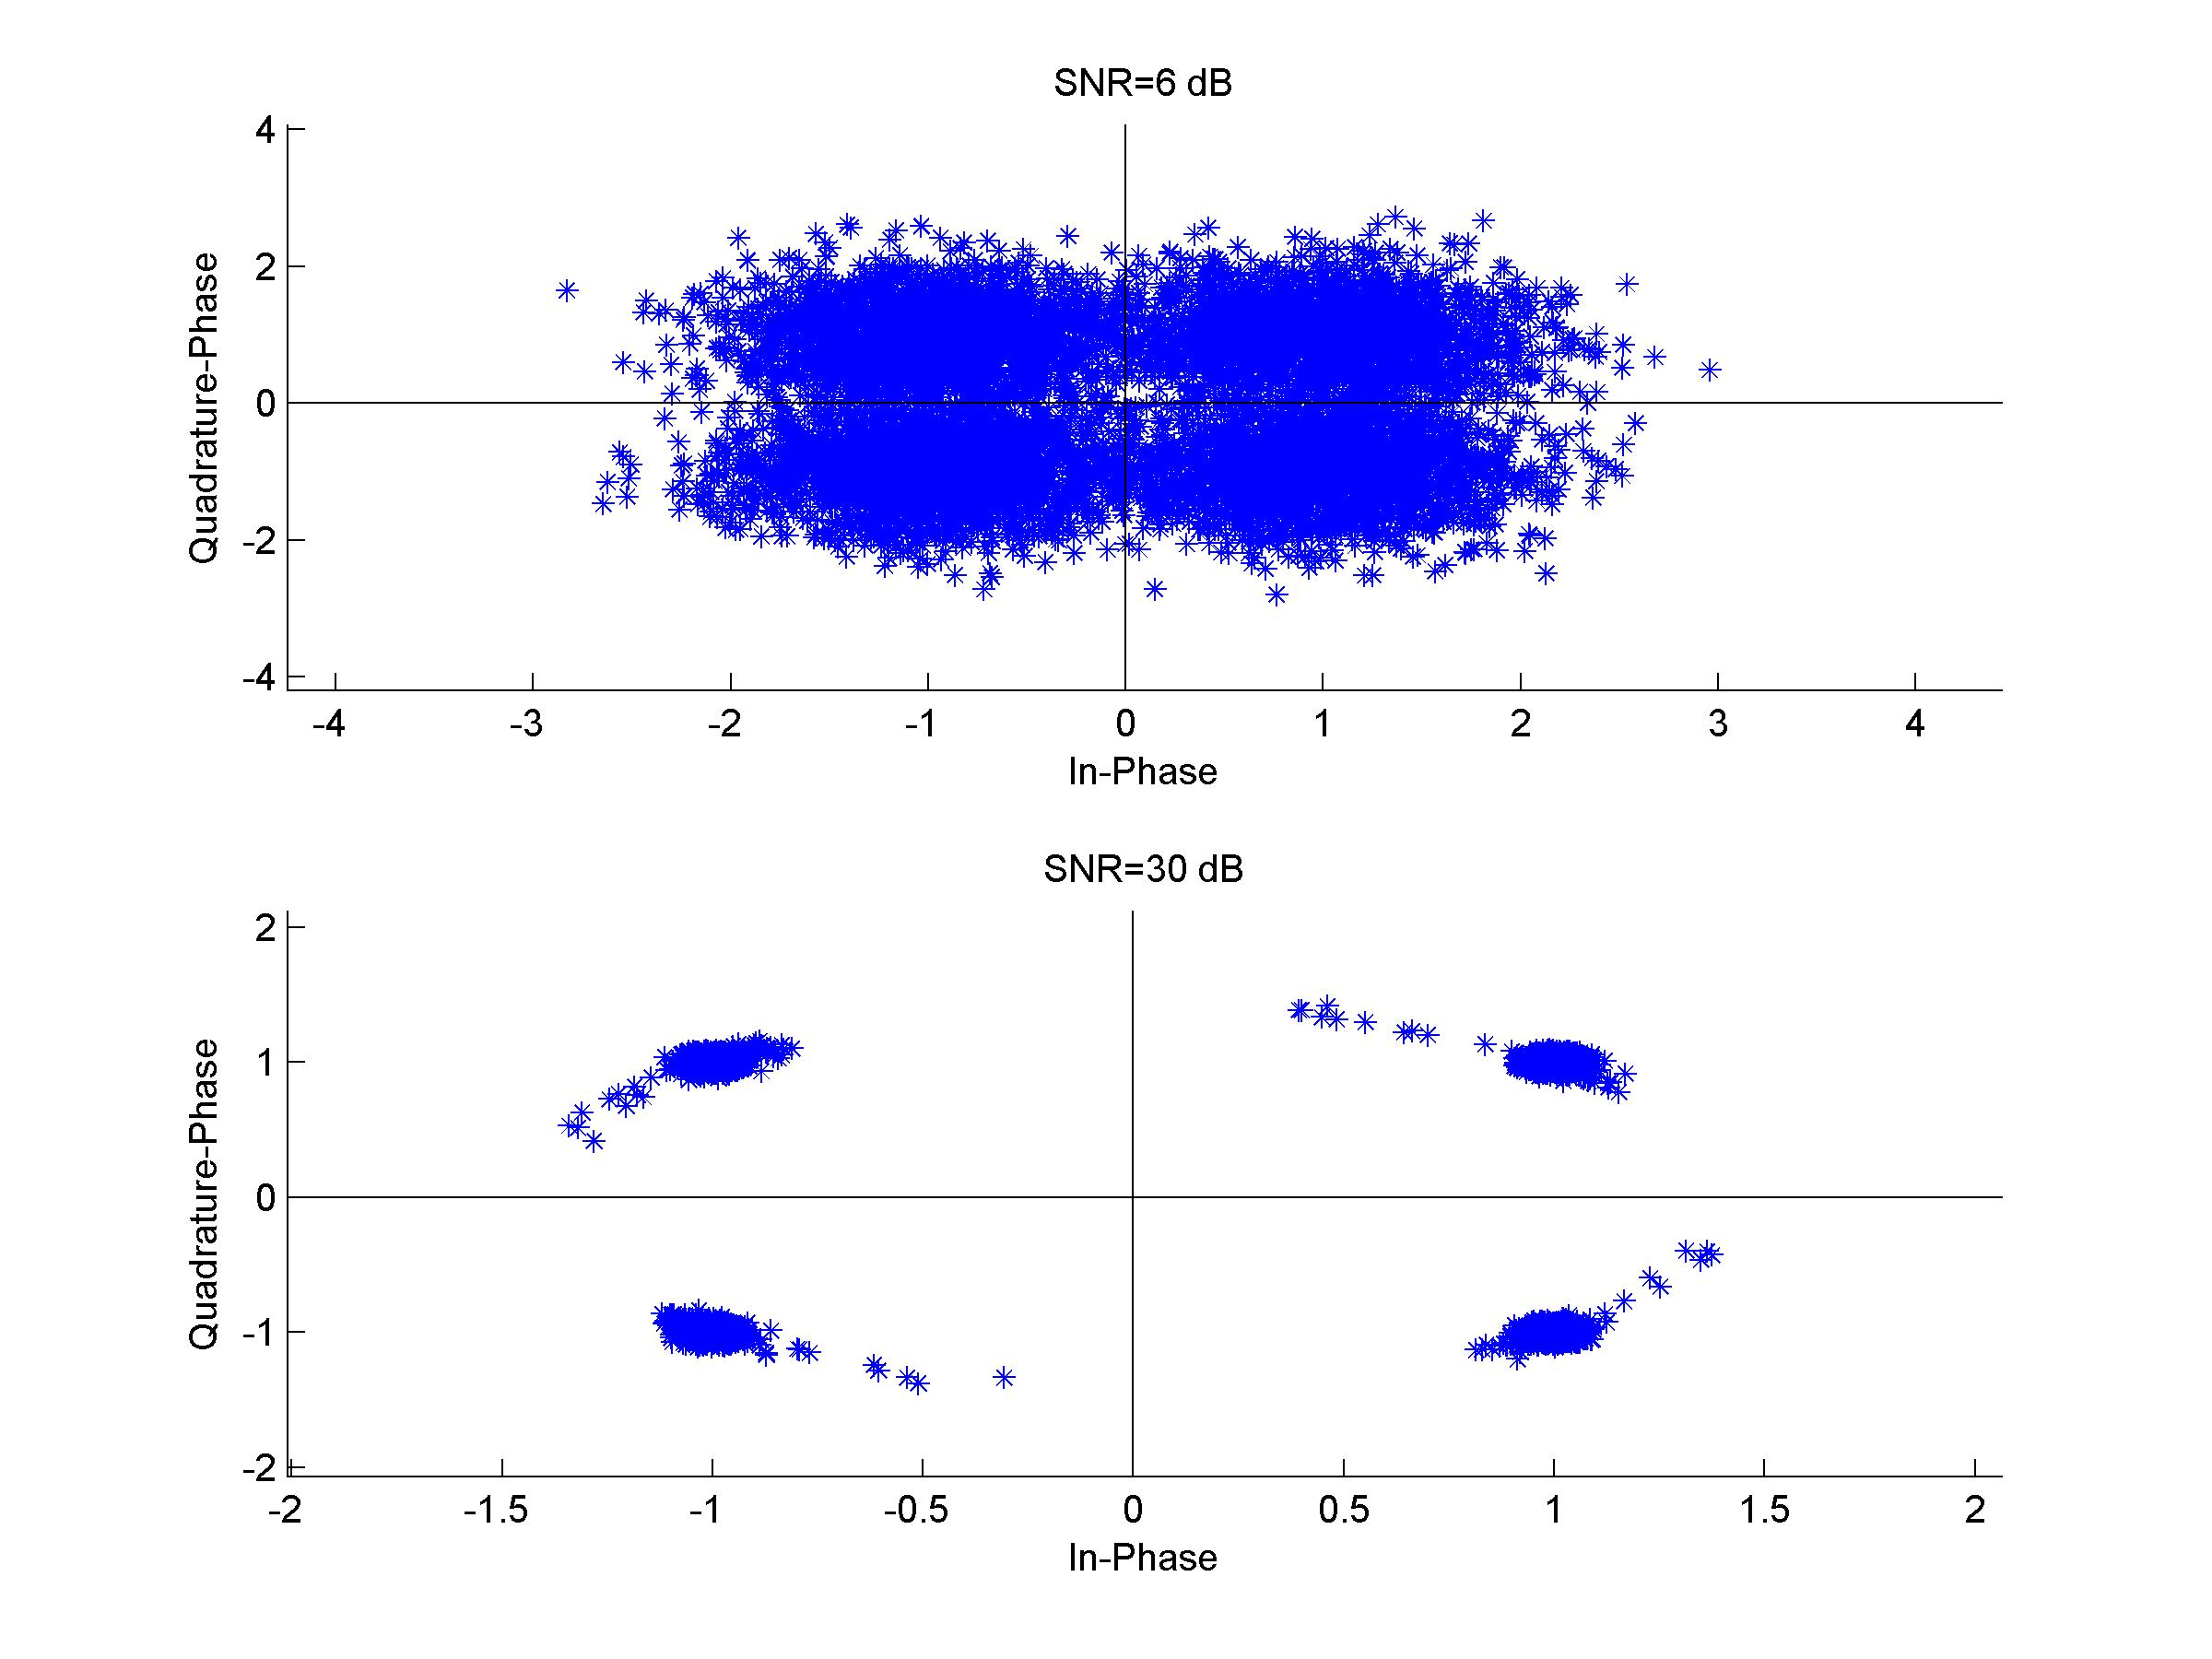
\includegraphics[width=0.7\textwidth]{qpConstpo_costas1.jpg}
\caption{The resulting constellation plot of the output of the system with Costas Loop for an input with 30 degrees phase offset at 6dB and 30dB SNR }
\end{figure}


\subsubsection{Constellation Plots  for Frequency Recovery}
\begin{figure}[H]
\centering
\hspace*{-2cm}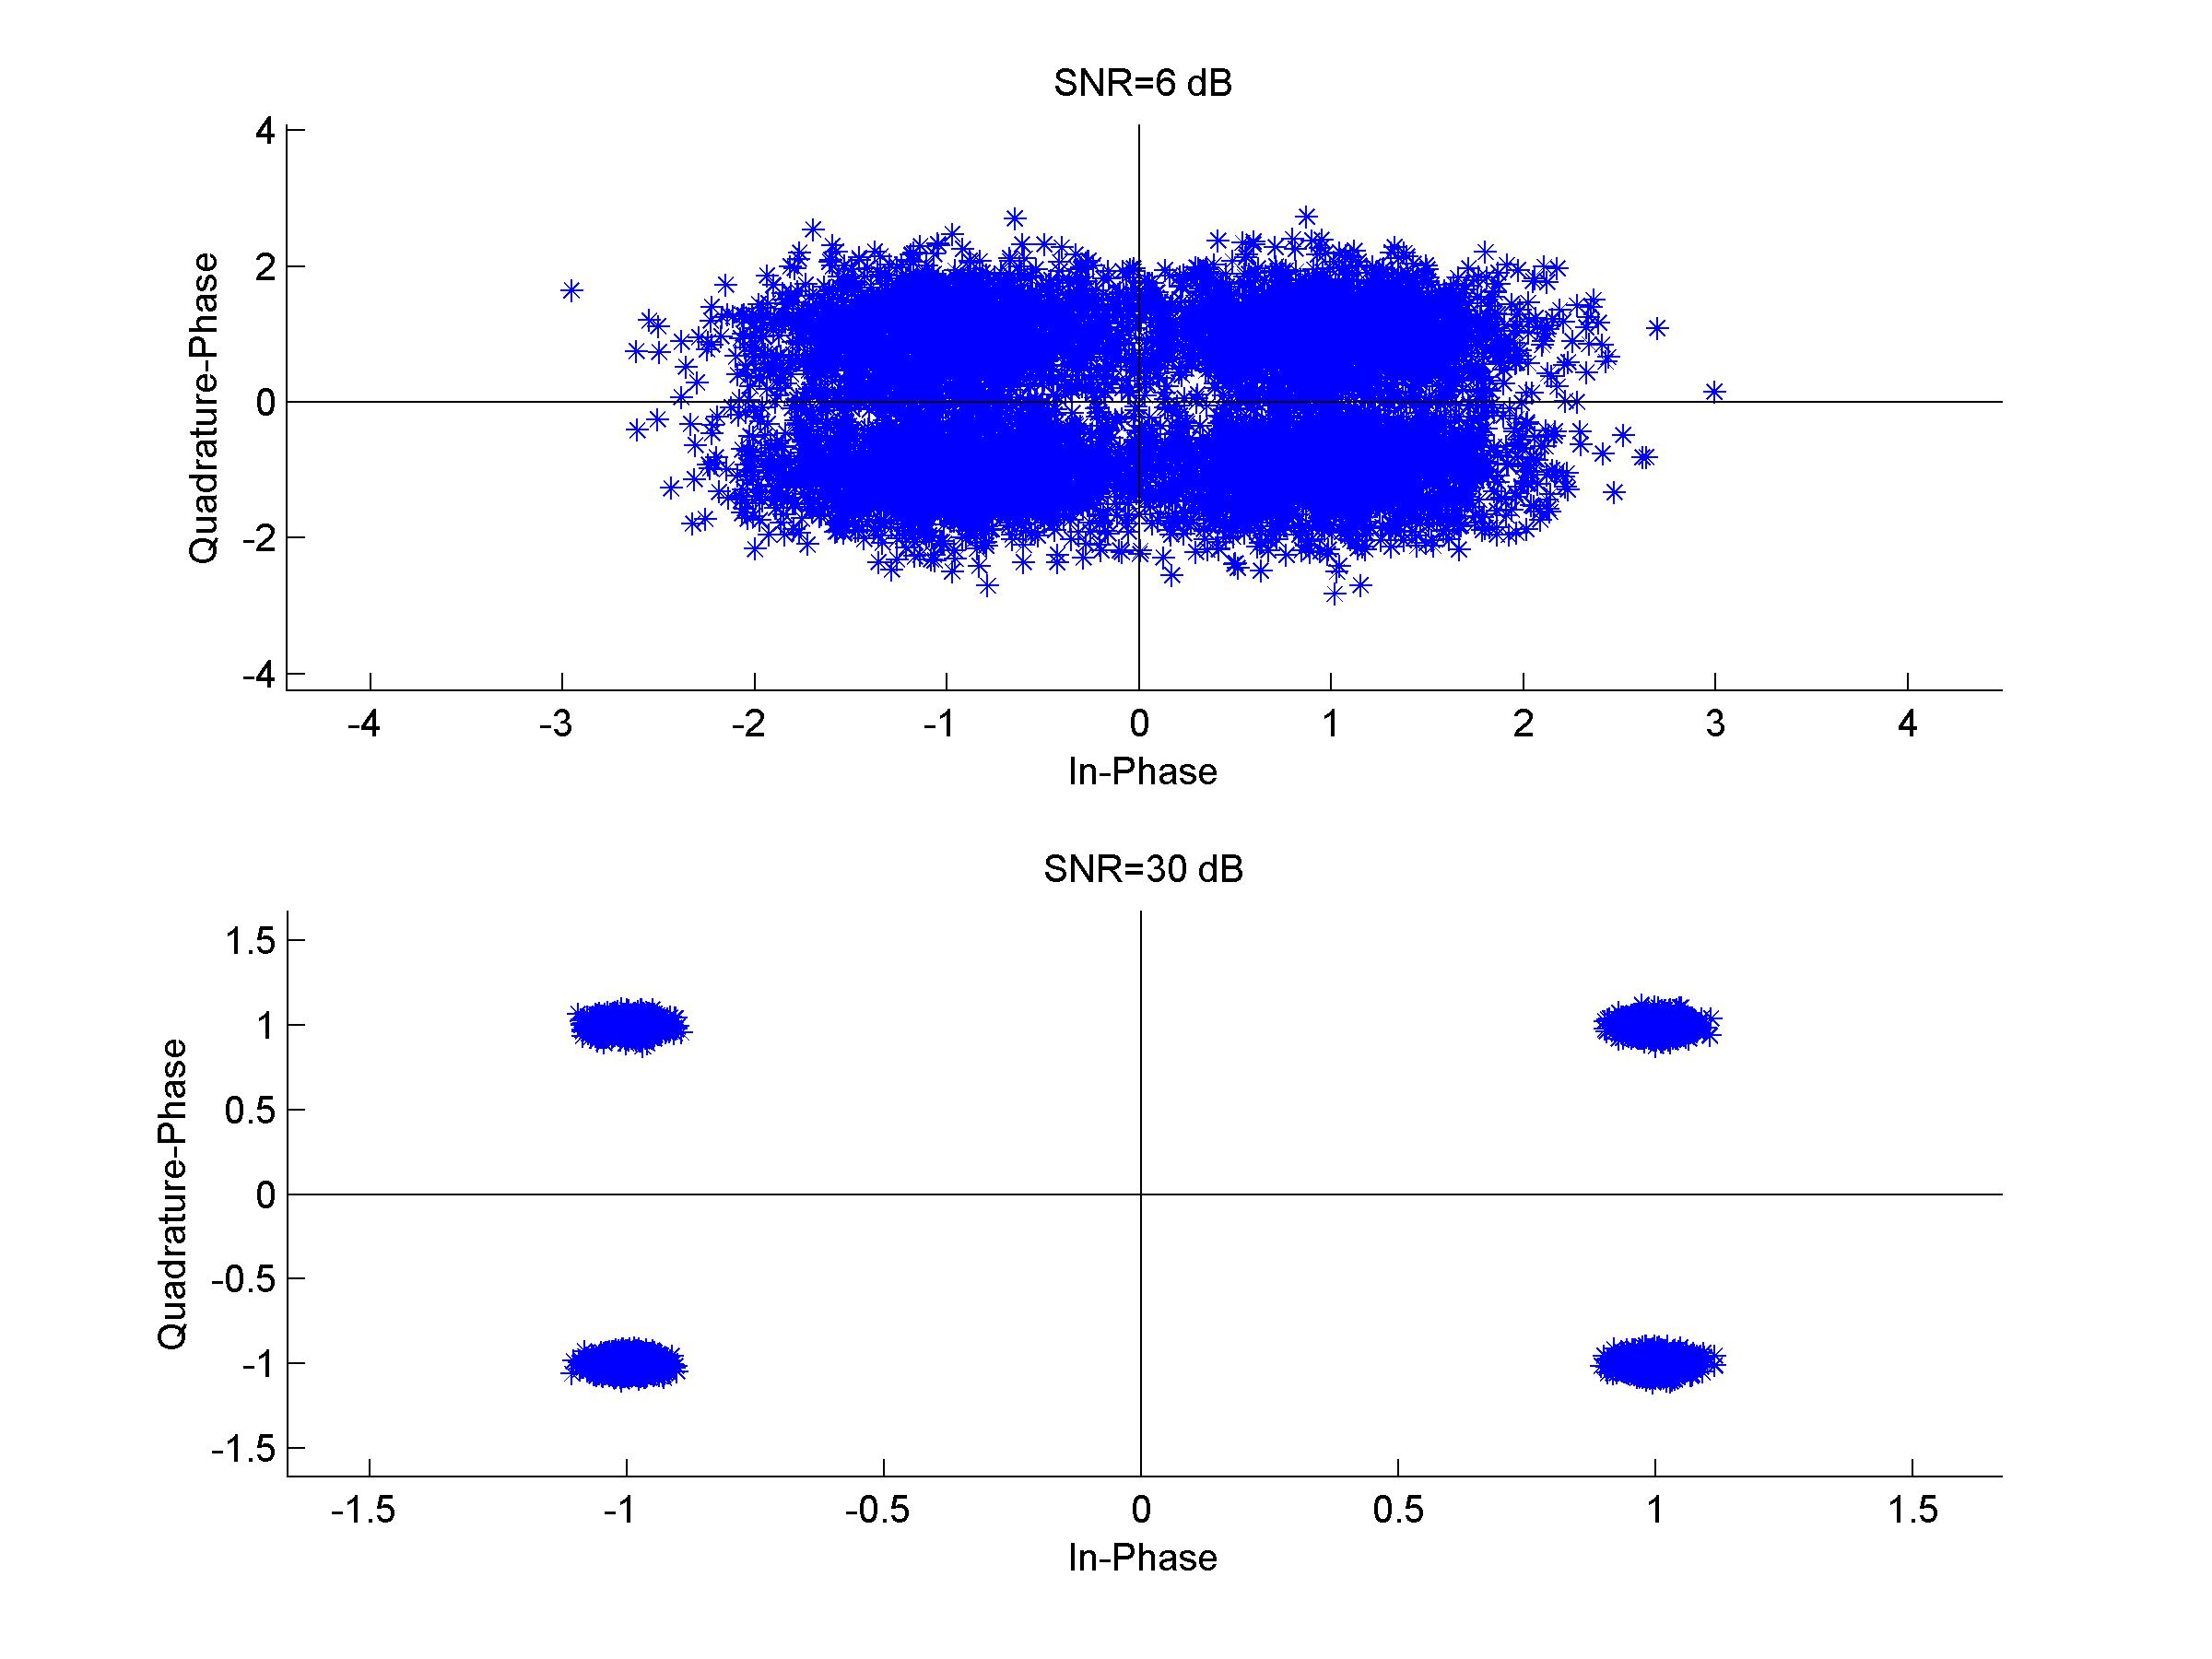
\includegraphics[width=0.7\textwidth]{qpConstfo_costas1.jpg}
\caption{The resulting constellation plot of the output of the system with Costas Loop for an input with 1ppm frequency offset at 6dB and 30dB SNR }
\end{figure}

\begin{figure}[H]
\centering
\hspace*{-2cm}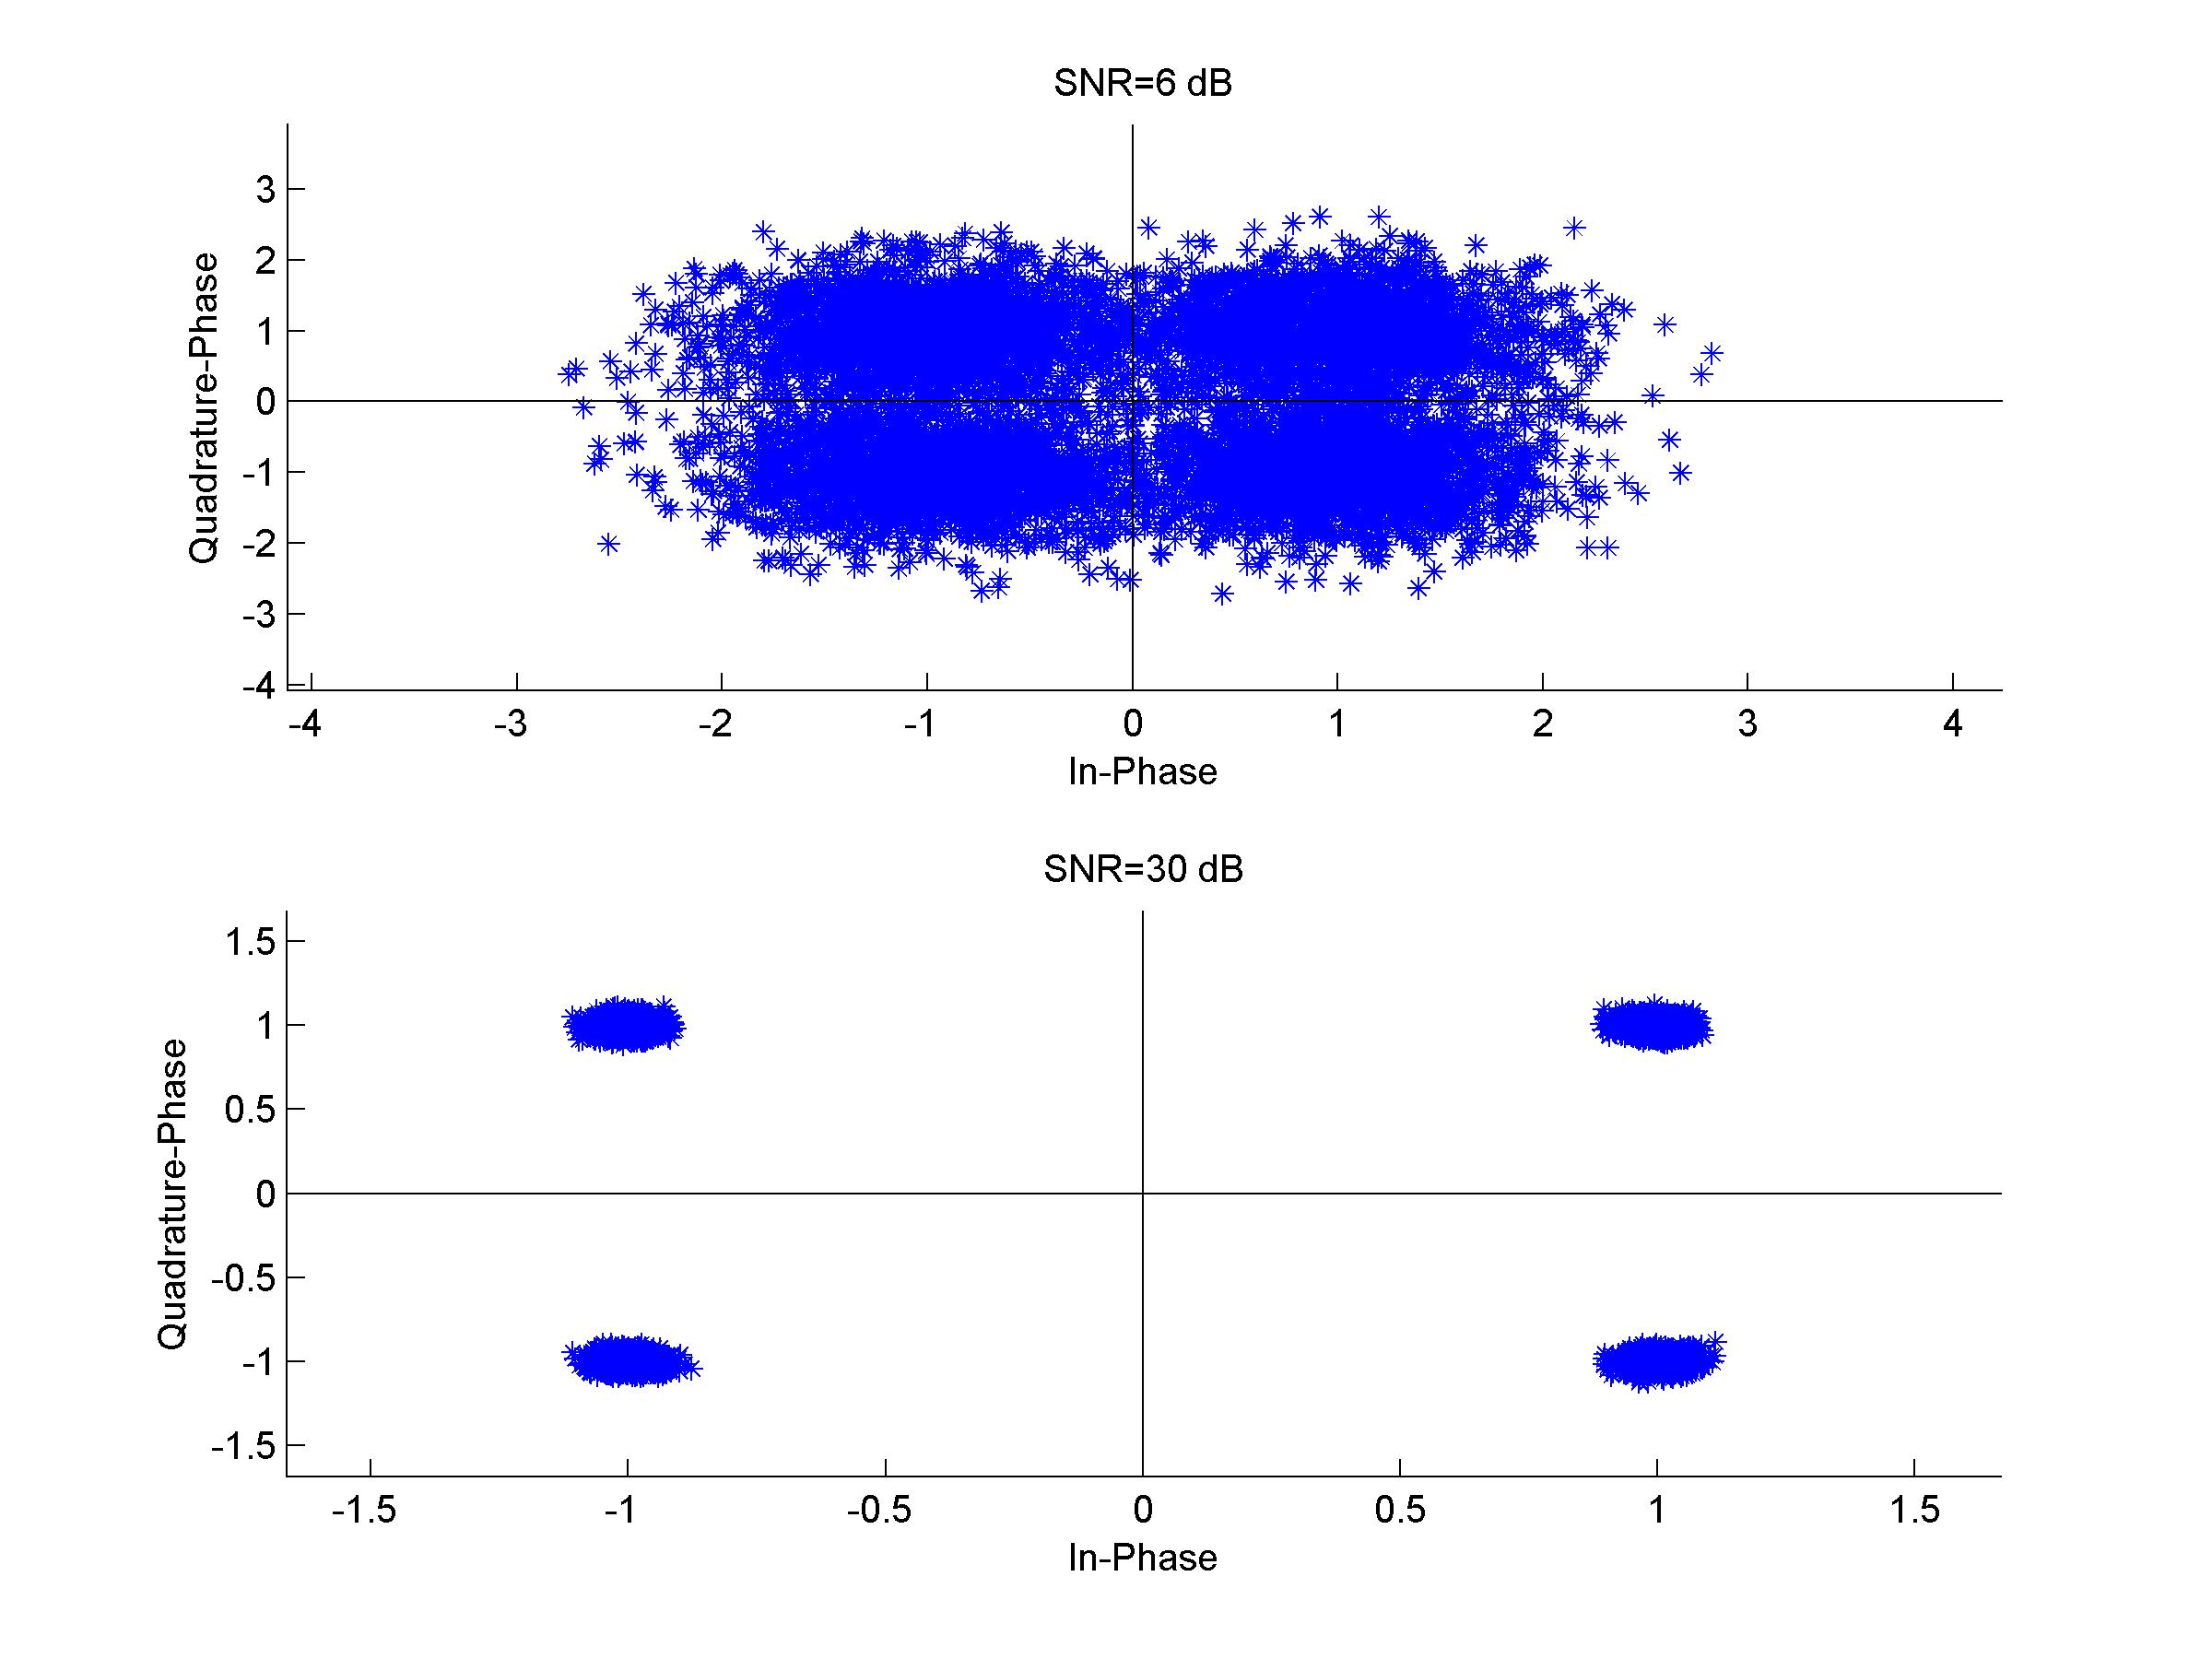
\includegraphics[width=0.7\textwidth]{qpConstfo_costas2.jpg}
\caption{The resulting constellation plot of the output of the system with Costas Loop for an input with 30 ppm frequency offset at 6dB and 30dB SNR }
\end{figure}


\subsubsection{BER Plots for Carrier Recovery}


\begin{figure}[H]
\centering
\hspace*{-2cm}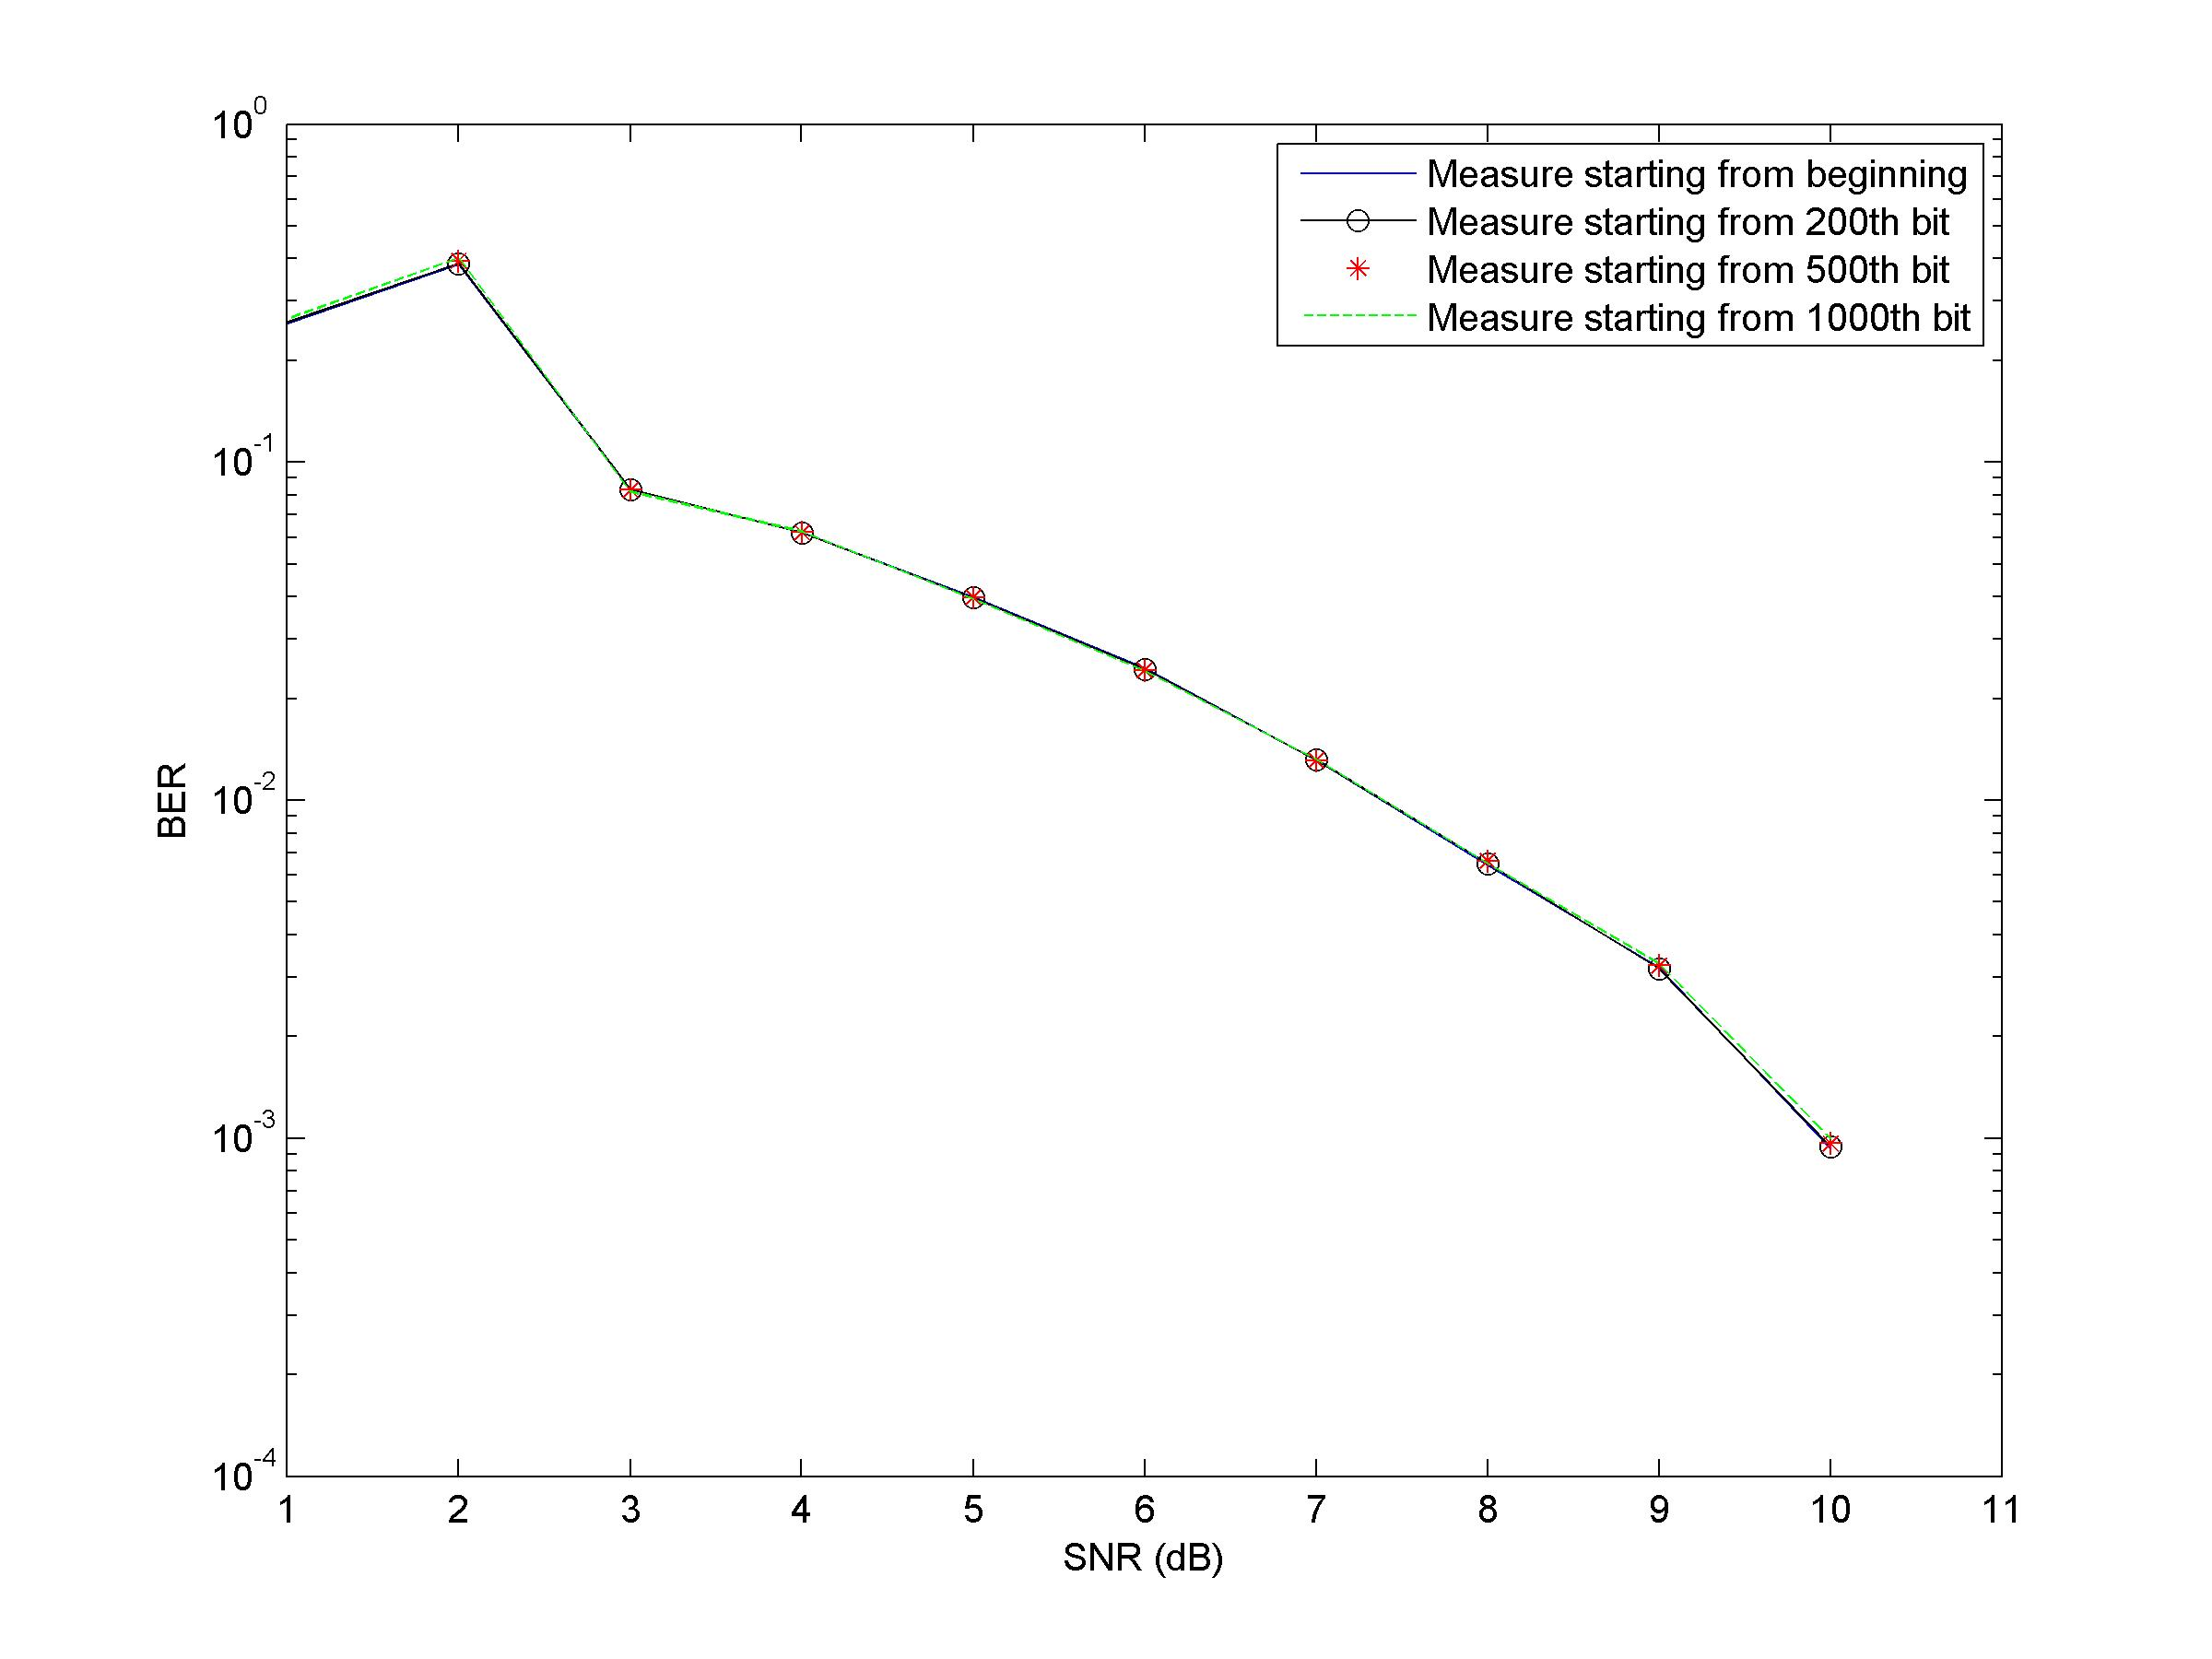
\includegraphics[width=0.7\textwidth]{qpBERfo_costas1.jpg}
\caption{BER plots of the system with Costas Loop for an input with 1ppm frequency offset (using output bits starting from different indices)}
\end{figure}

\begin{figure}[H]
\centering
\hspace*{-2cm}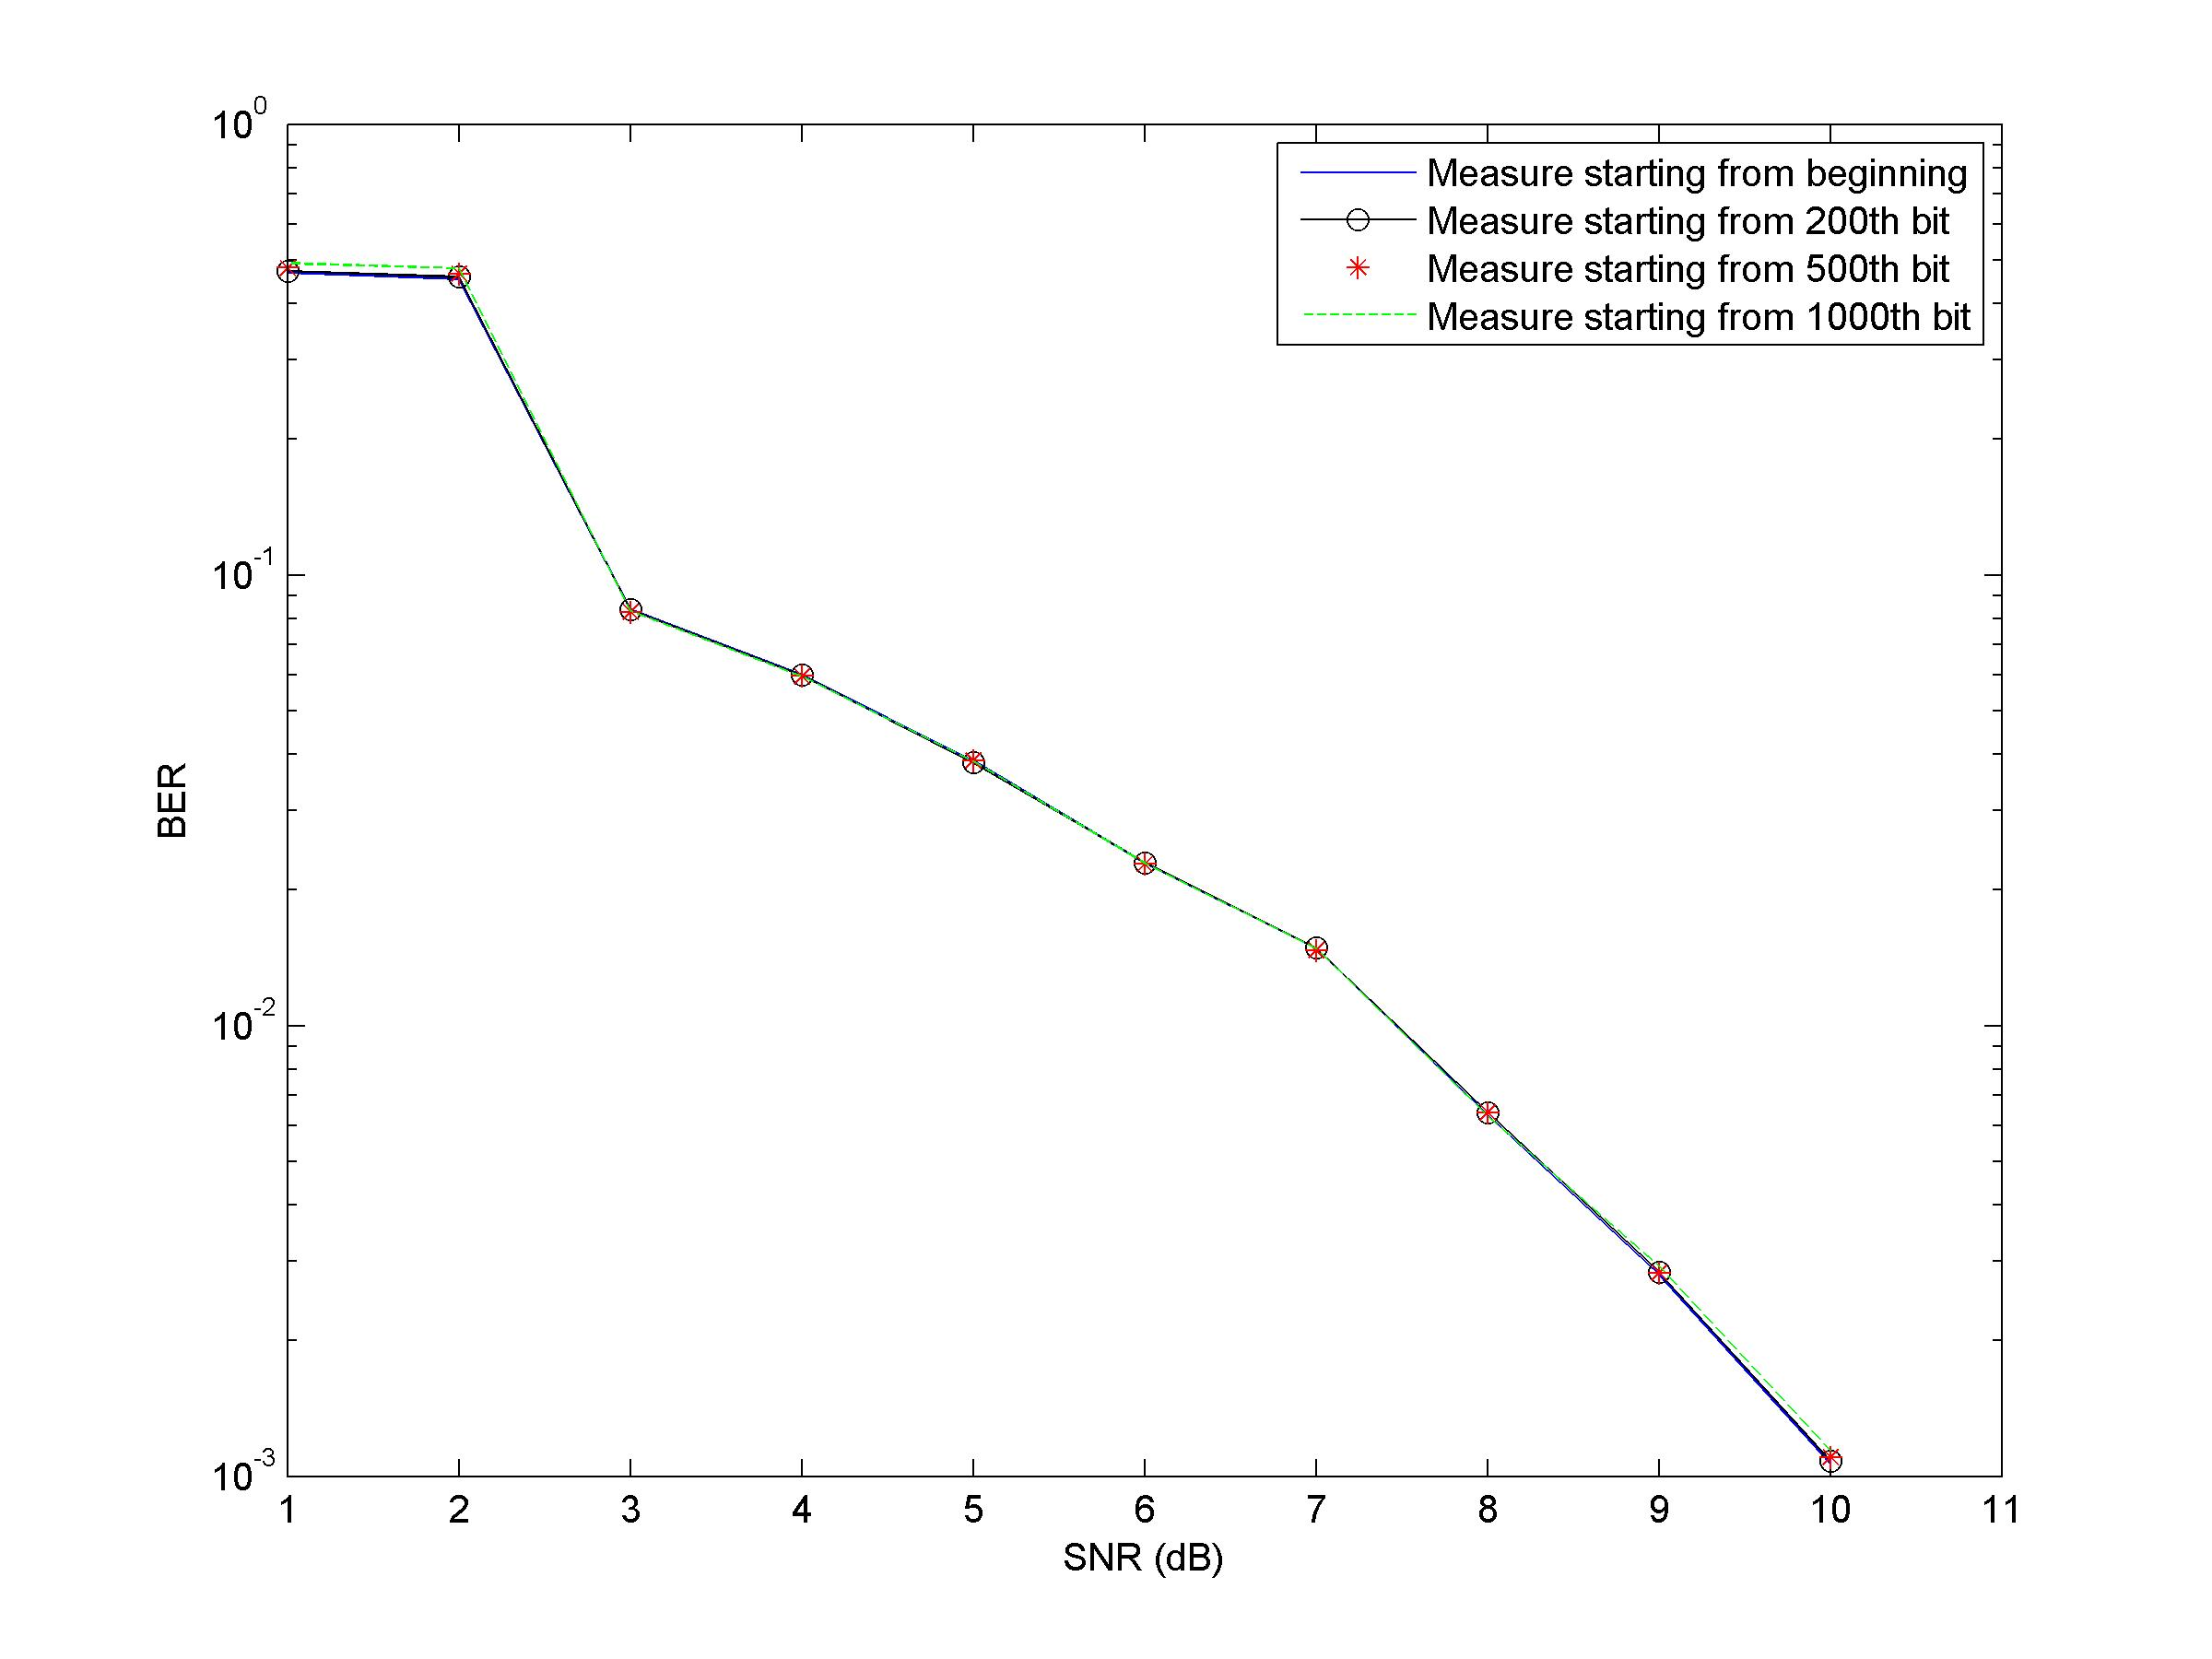
\includegraphics[width=0.7\textwidth]{qpBERfo_costas2.jpg}
\caption{BER plots of the system with Costas Loop for an input with 30ppm frequency offset (using output bits starting from different indices)}
\end{figure}

\subsubsection{BER Plots for Phase Recovery}
\begin{figure}[H]
\centering
\hspace*{-2cm}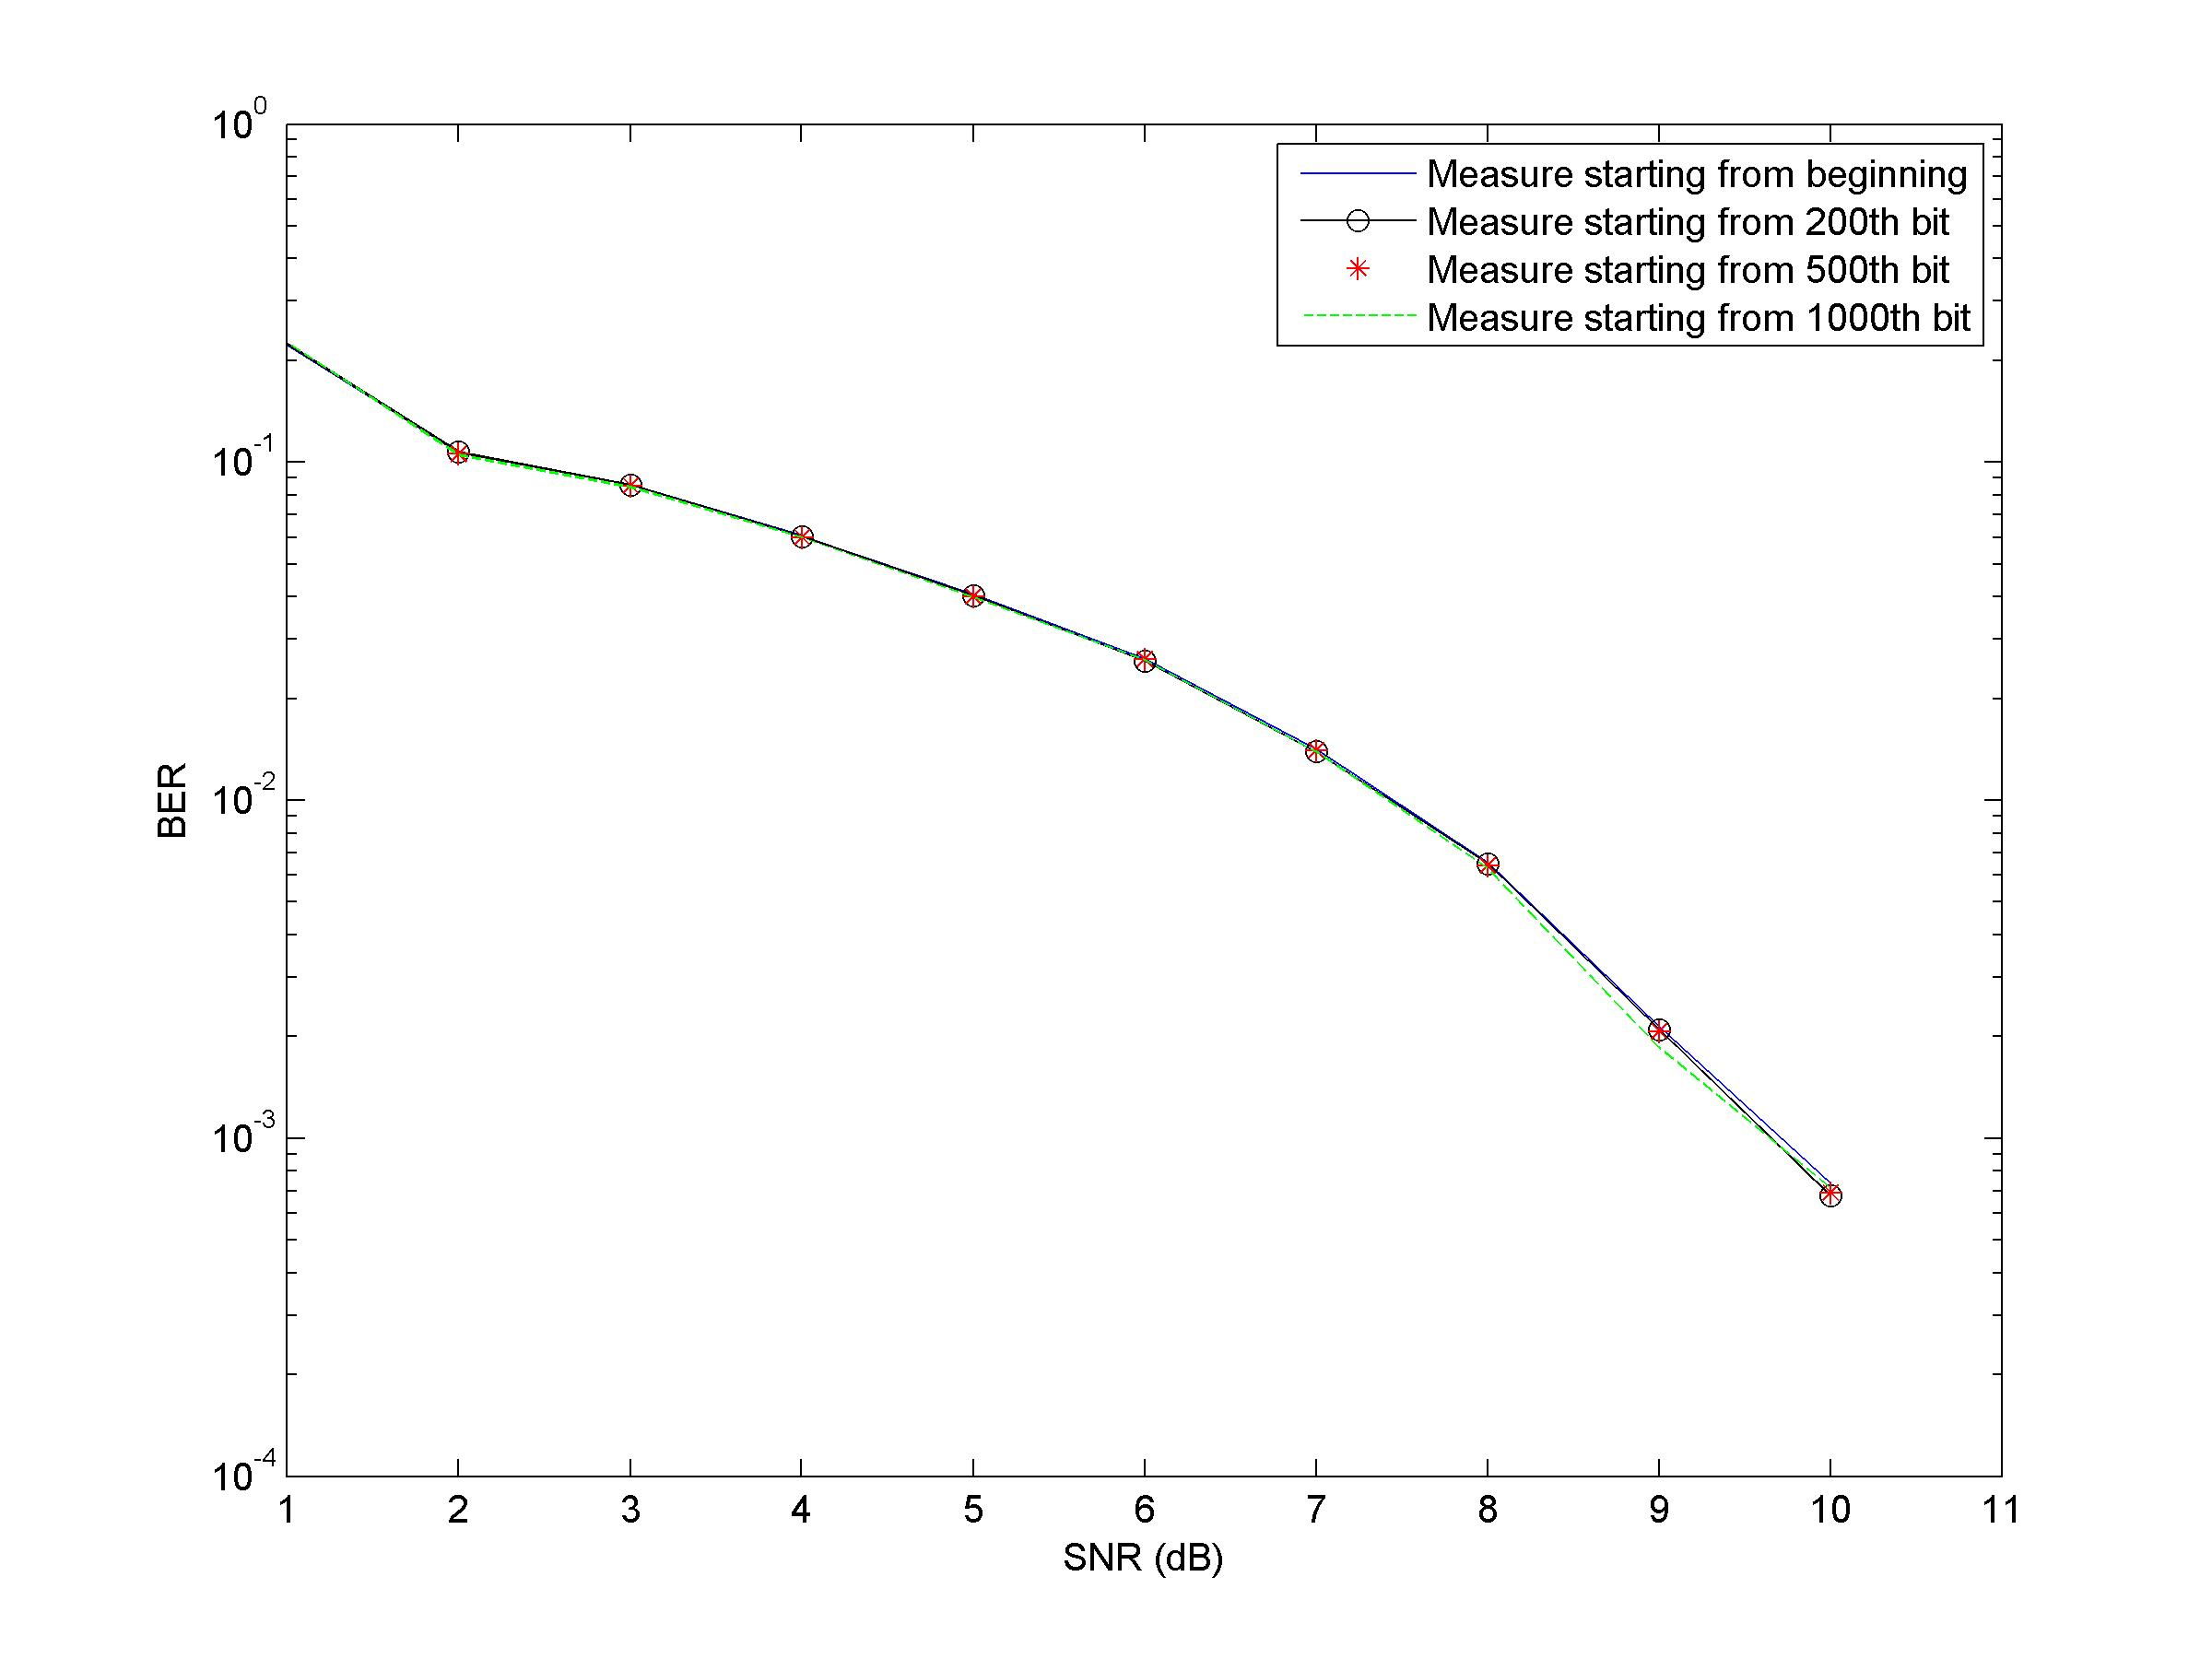
\includegraphics[width=0.7\textwidth]{qpBERpo_costas1.jpg}
\caption{BER plots of the system with Costas Loop for an input with 30 degrees phase offset (using output bits starting from different indices)}
\end{figure}

\subsection{QPSK with Decision Directed Recovery}

\subsubsection{S-Curve of Phase Detector}
\begin{figure}[H]
\centering
\hspace*{-2cm}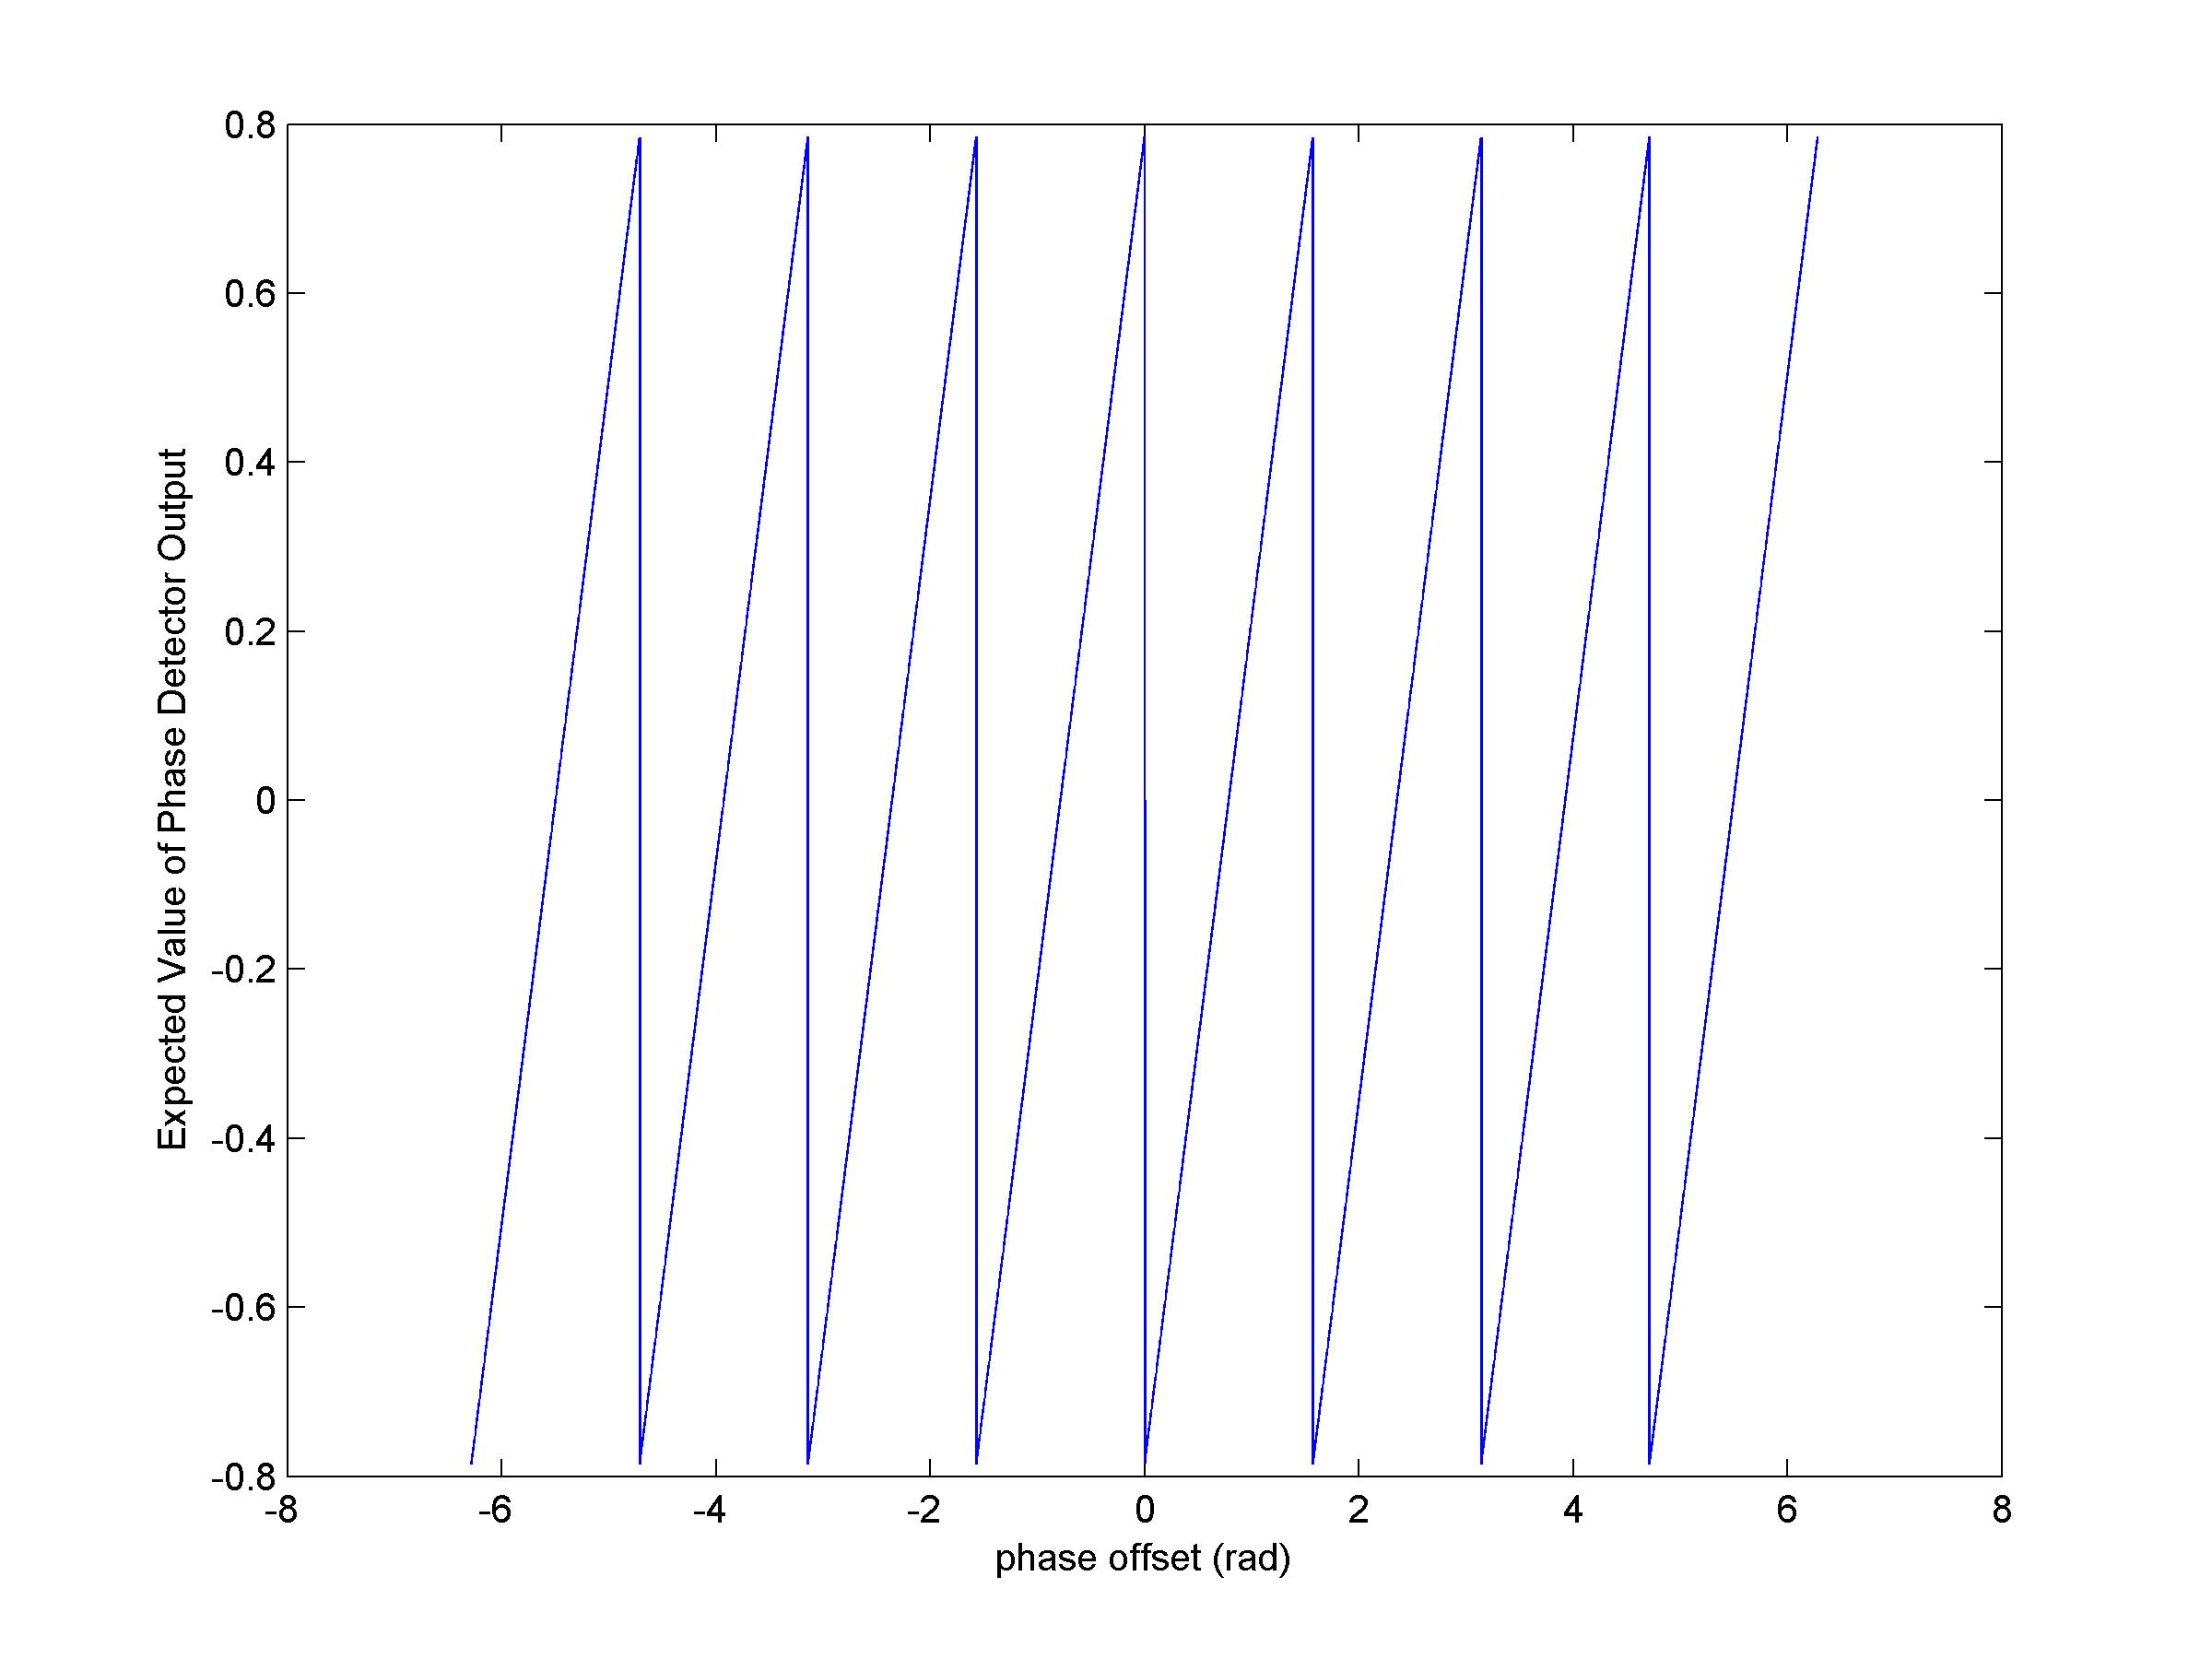
\includegraphics[width=0.7\textwidth]{qpScurvepo_ddr.jpg}
\caption{S-curve of the phase detector used in Decision Directed Recovery Loop}
\end{figure}
\subsubsection{S-Curve of Carrier Detector}
\begin{figure}[H]
\centering
\hspace*{-2cm}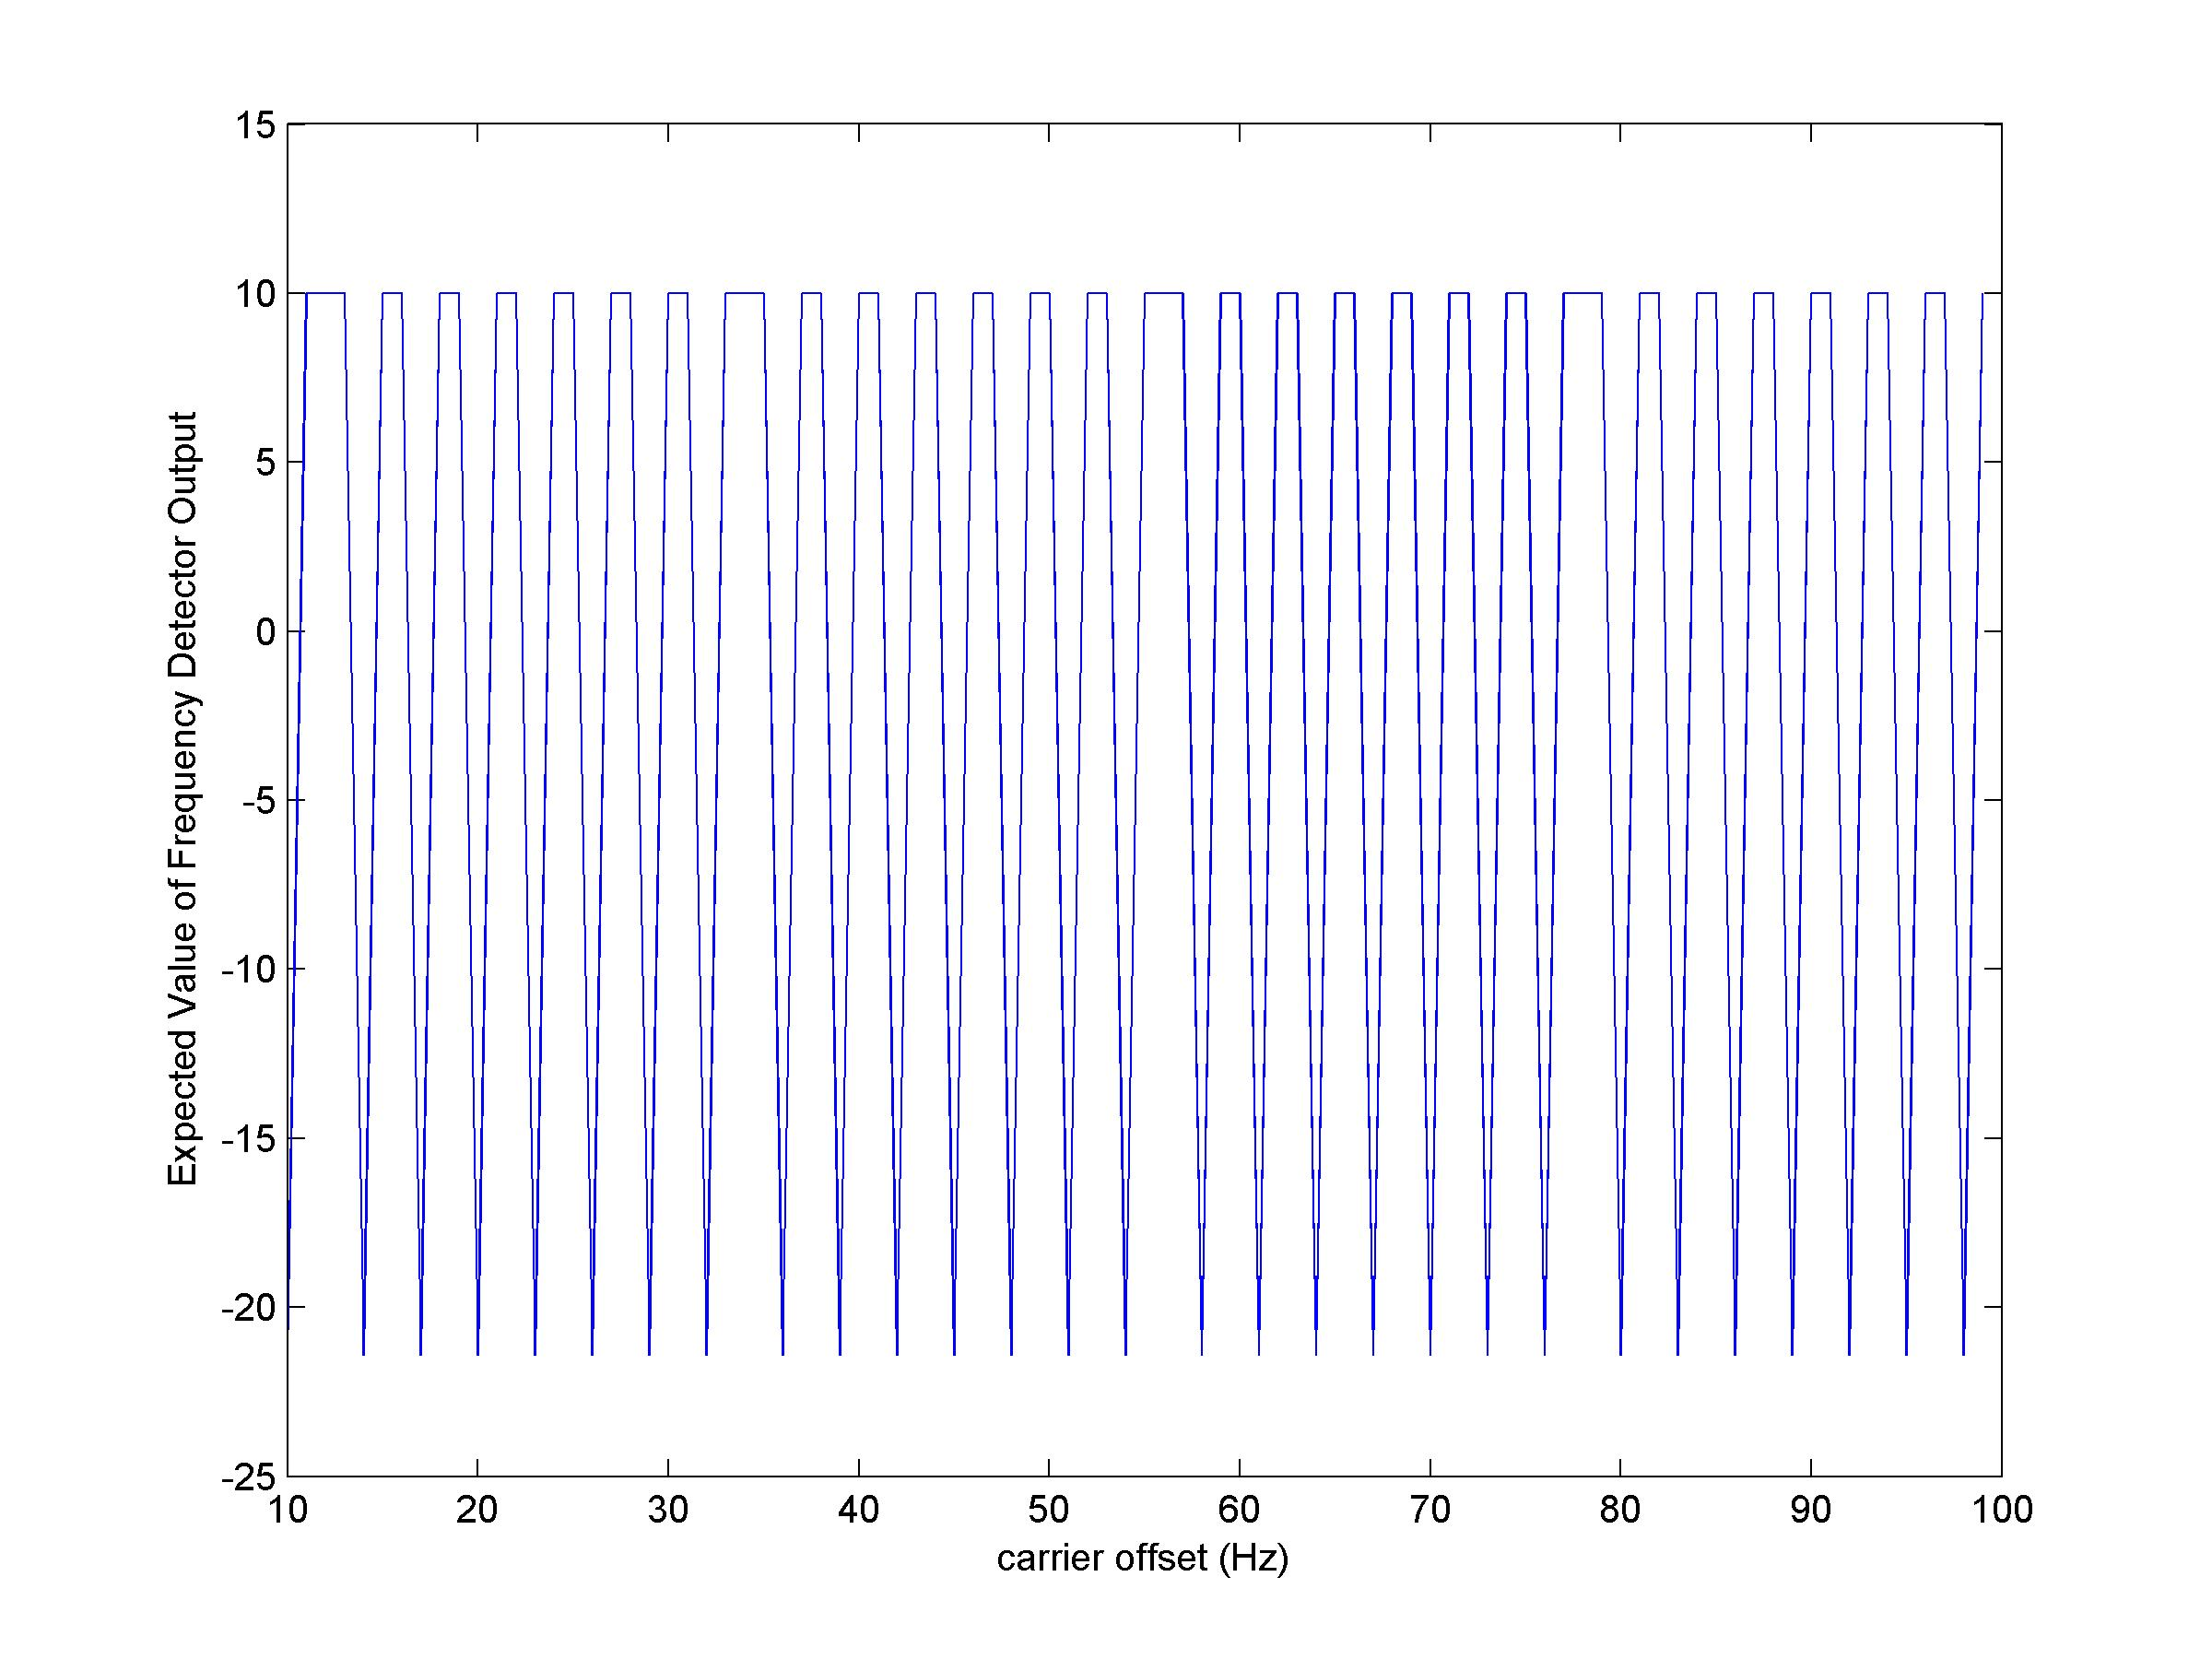
\includegraphics[width=0.7\textwidth]{qpScurvefo.jpg}
\caption{S-curve of the frequency detector used in Decision Directed Recovery Loop}
\end{figure}

\subsubsection{Transience of Phase Recovery}
\begin{figure}[H]
\centering
\hspace*{-2cm}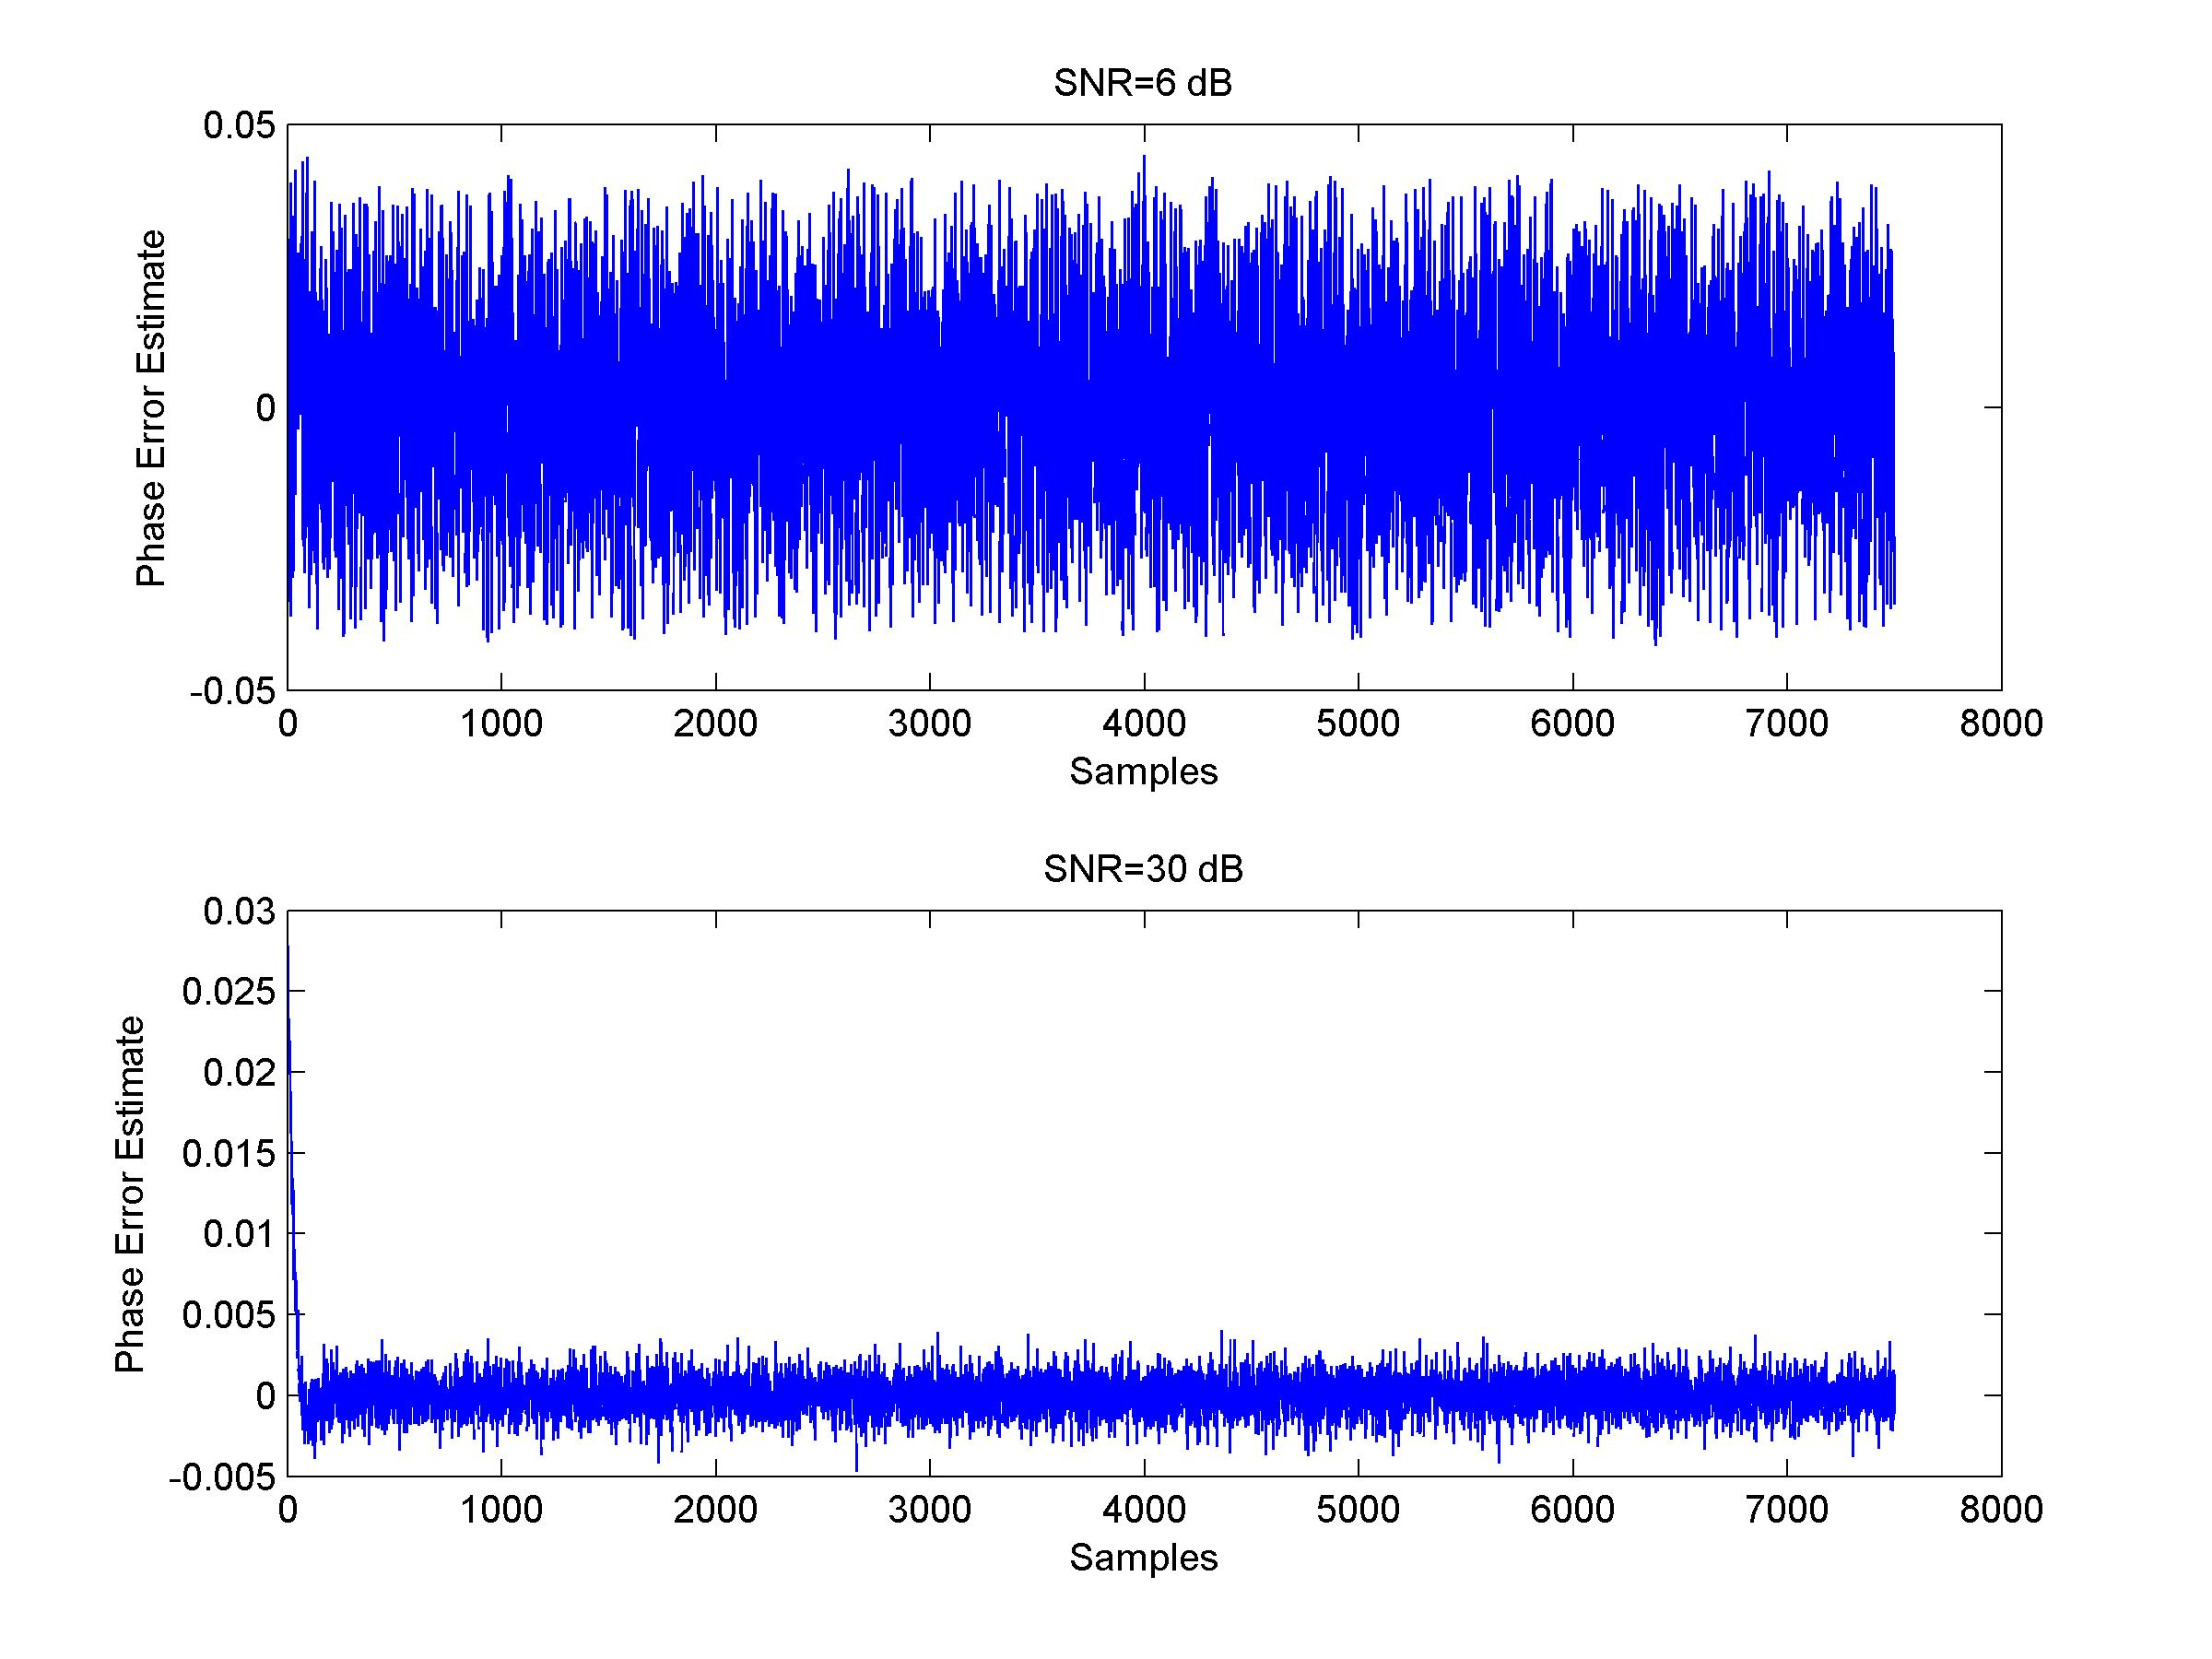
\includegraphics[width=0.7\textwidth]{qpLoopFilterpo_ddr1.jpg}
\caption{The loop filter output of the Decision Directed Recovery Loop for an input signal with 30 degrees phase offset}
\end{figure}

\subsubsection{Transience of Carrier Recovery}
\begin{figure}[H]
\centering
\hspace*{-2cm}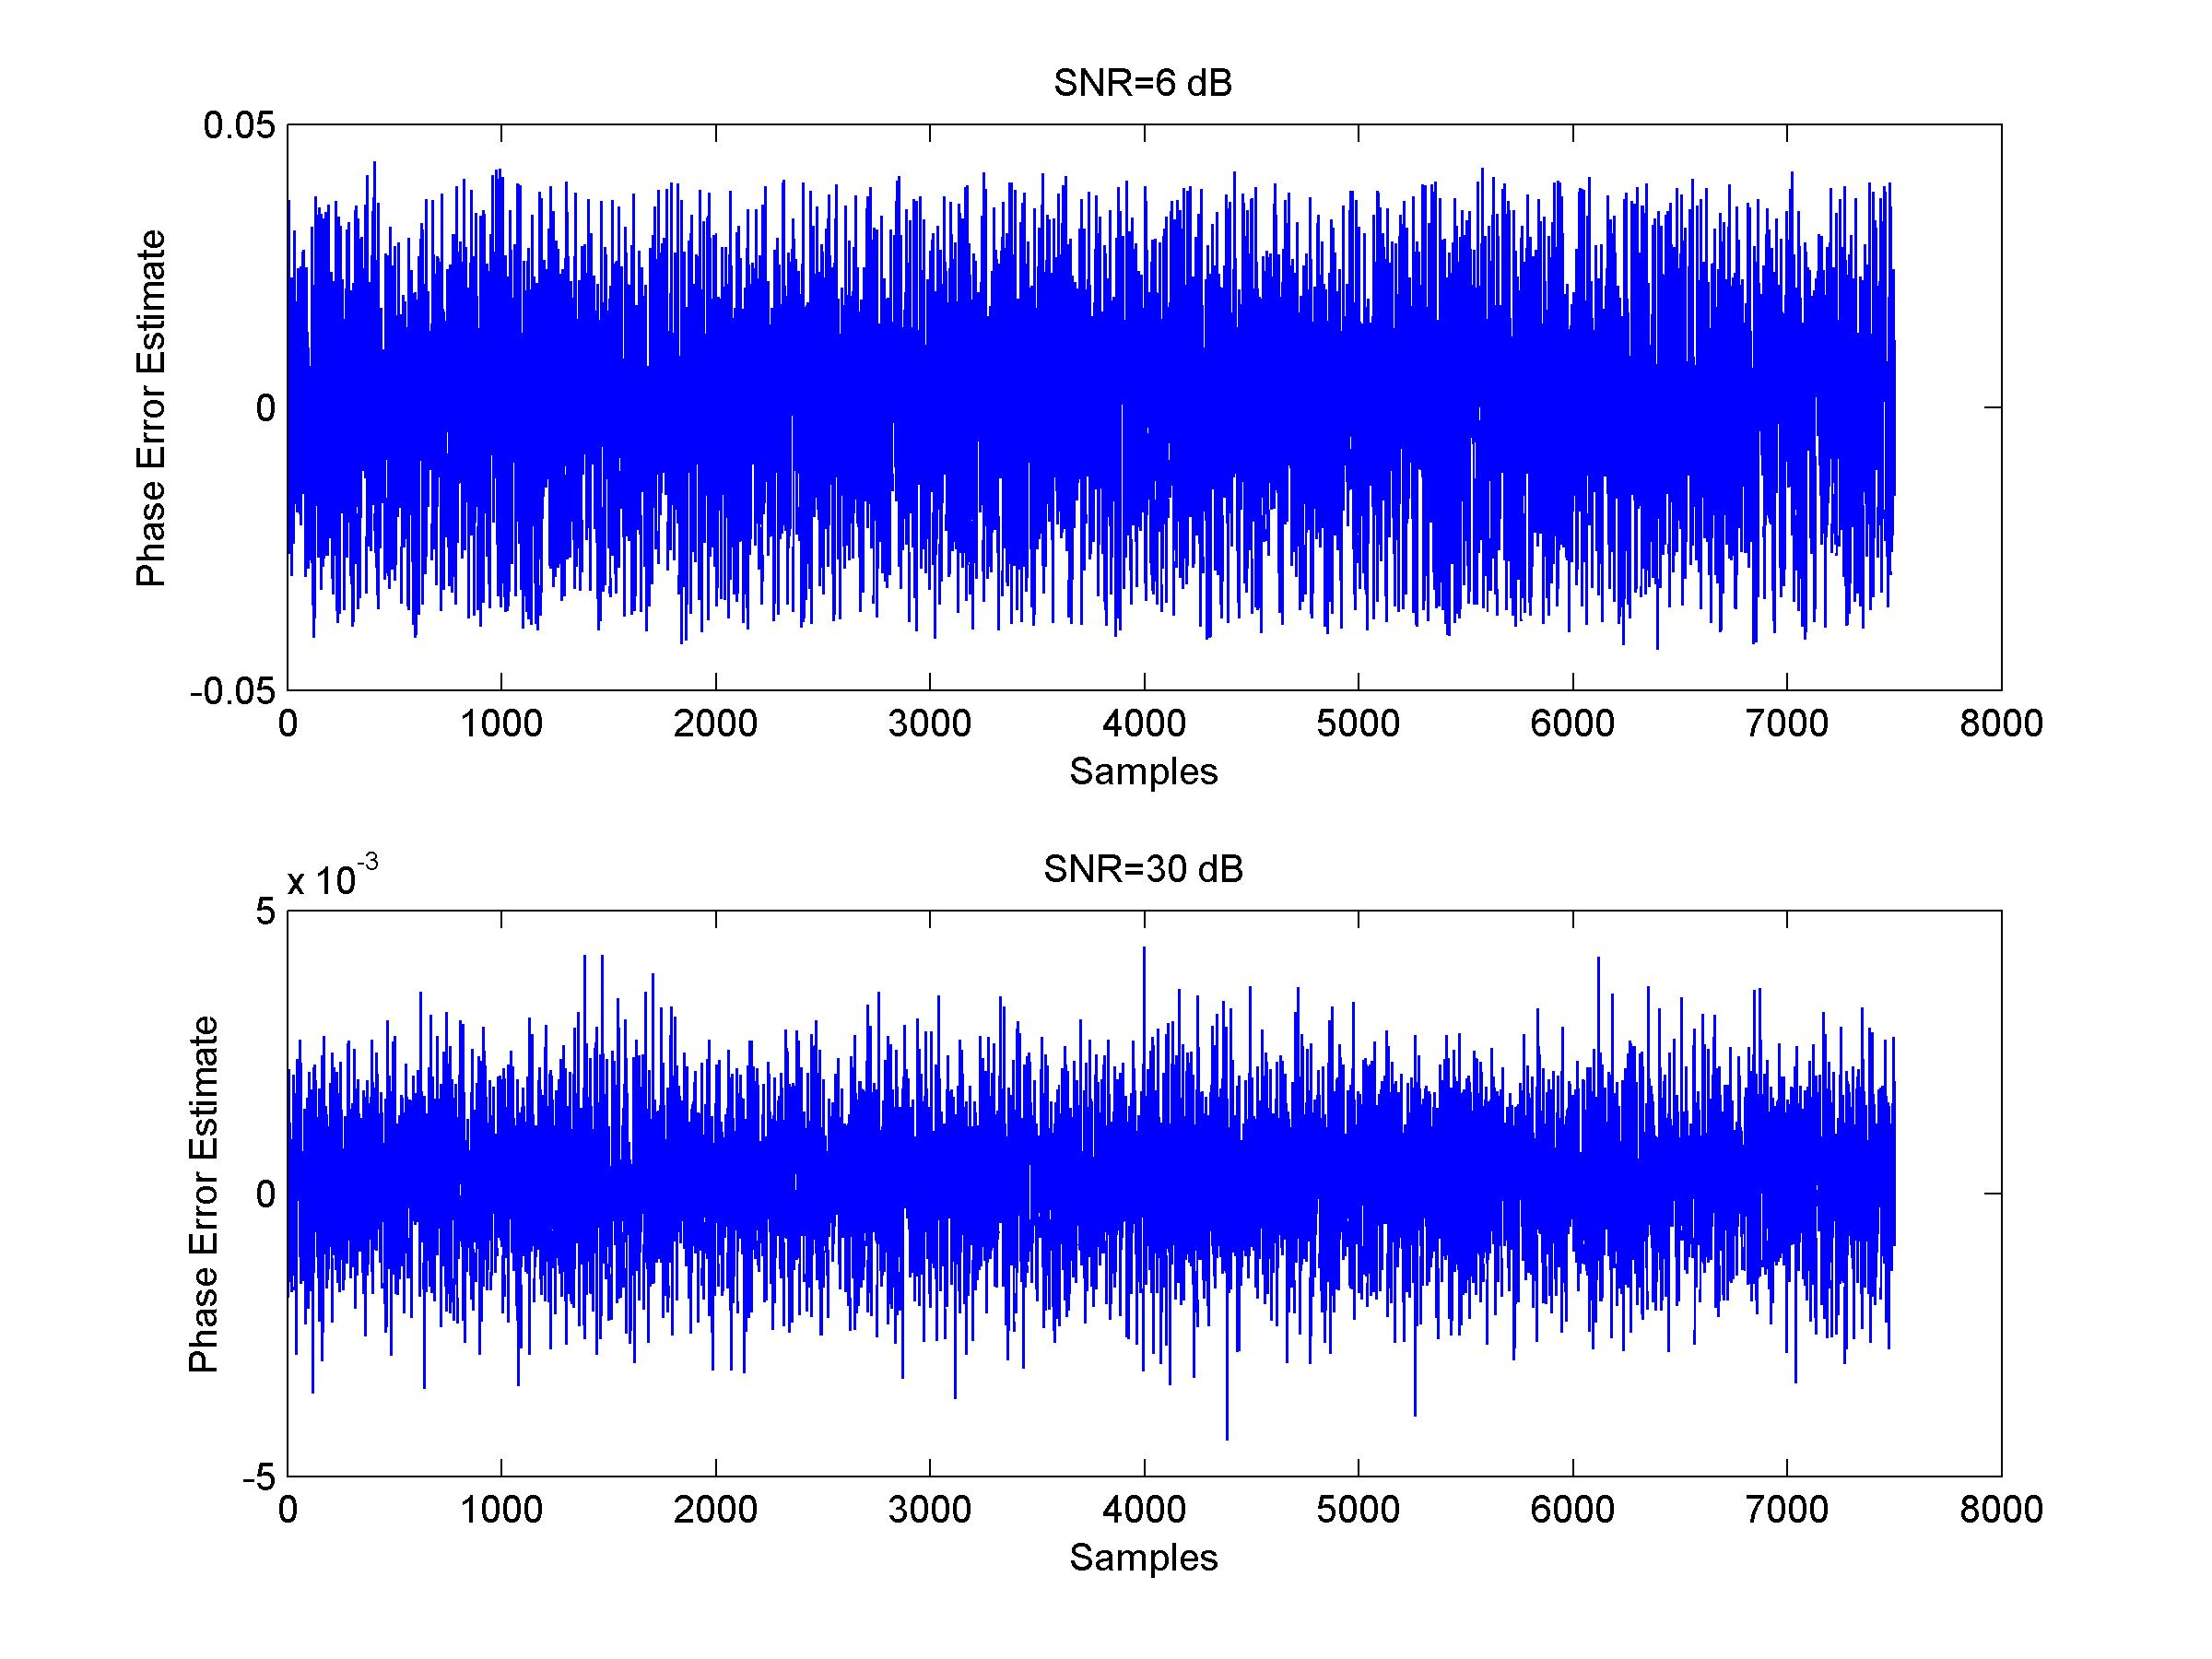
\includegraphics[width=0.7\textwidth]{qpLoopFilterfo_ddr1.jpg}
\caption{The loop filter output of the Decision Directed Recovery Loop for an input signal with 1ppm frequency offset}
\end{figure}

\begin{figure}[H]
\centering
\hspace*{-2cm}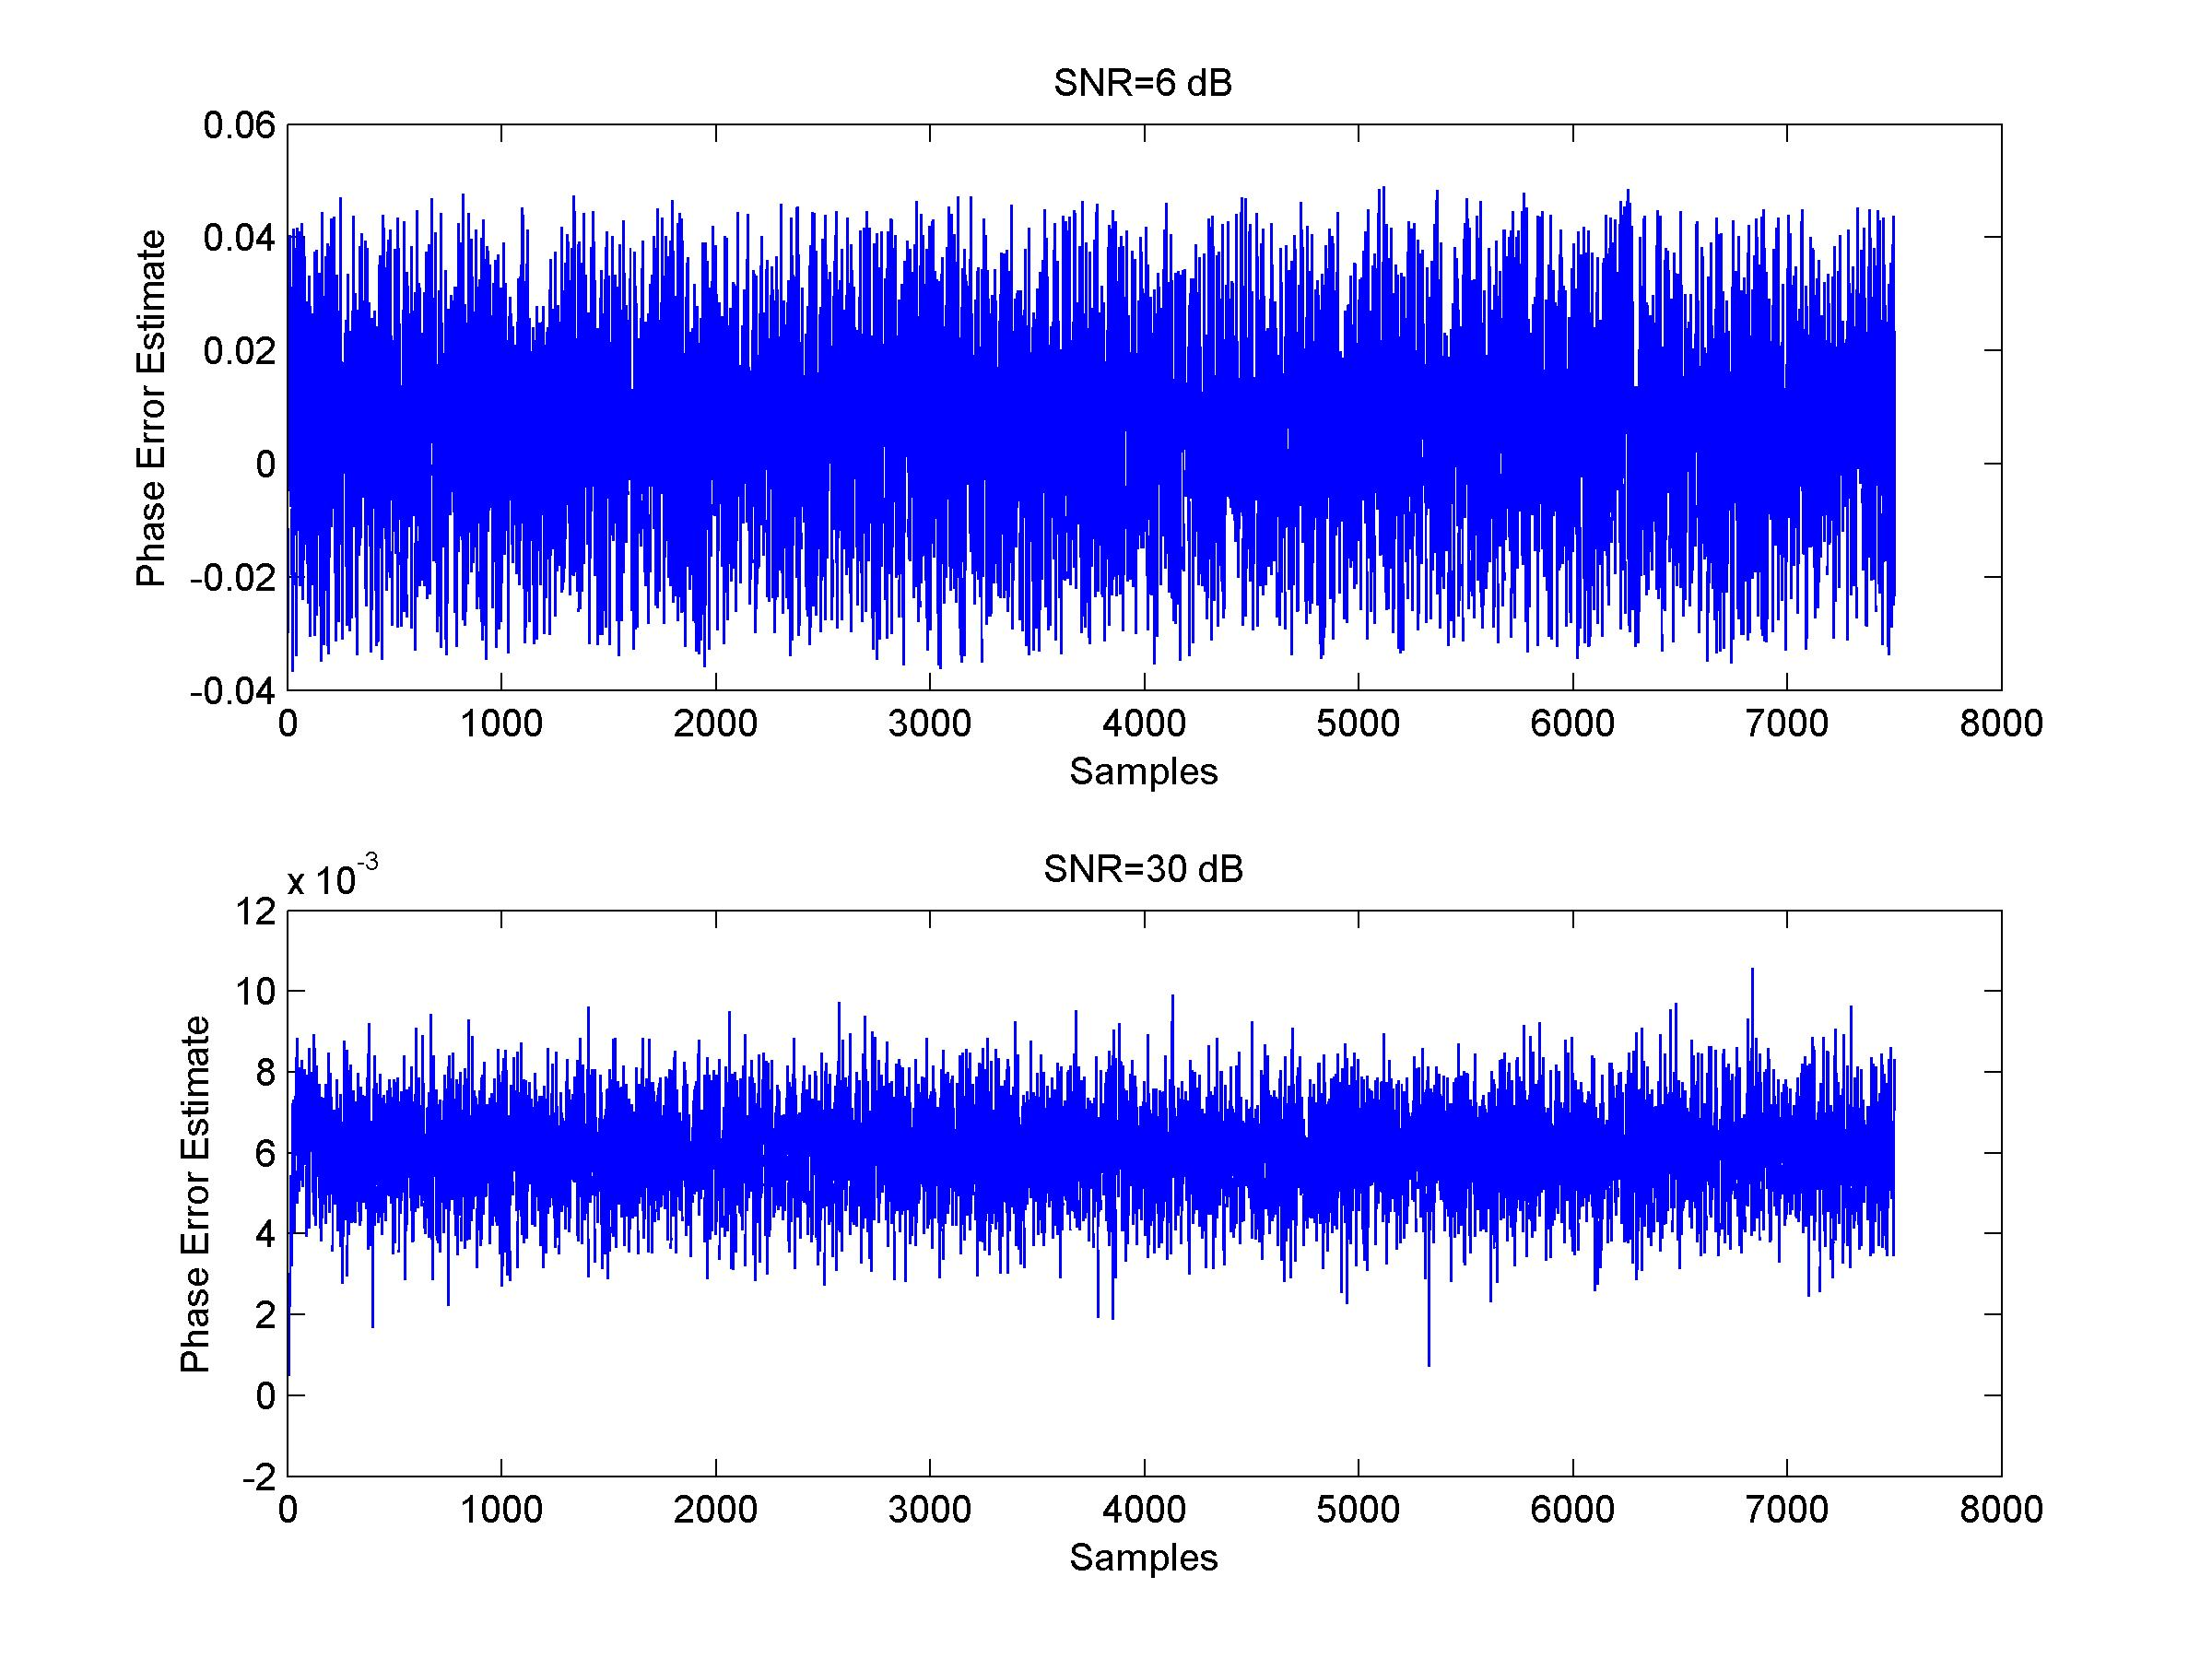
\includegraphics[width=0.7\textwidth]{qpLoopFilterfo_ddr2.jpg}
\caption{The loop filter output of the Decision Directed Recovery Loop for an input signal with 30ppm frequency offset}
\end{figure}

\subsubsection{Constellation Plots  for Phase Recovery}
\begin{figure}[H]
\centering
\hspace*{-2cm}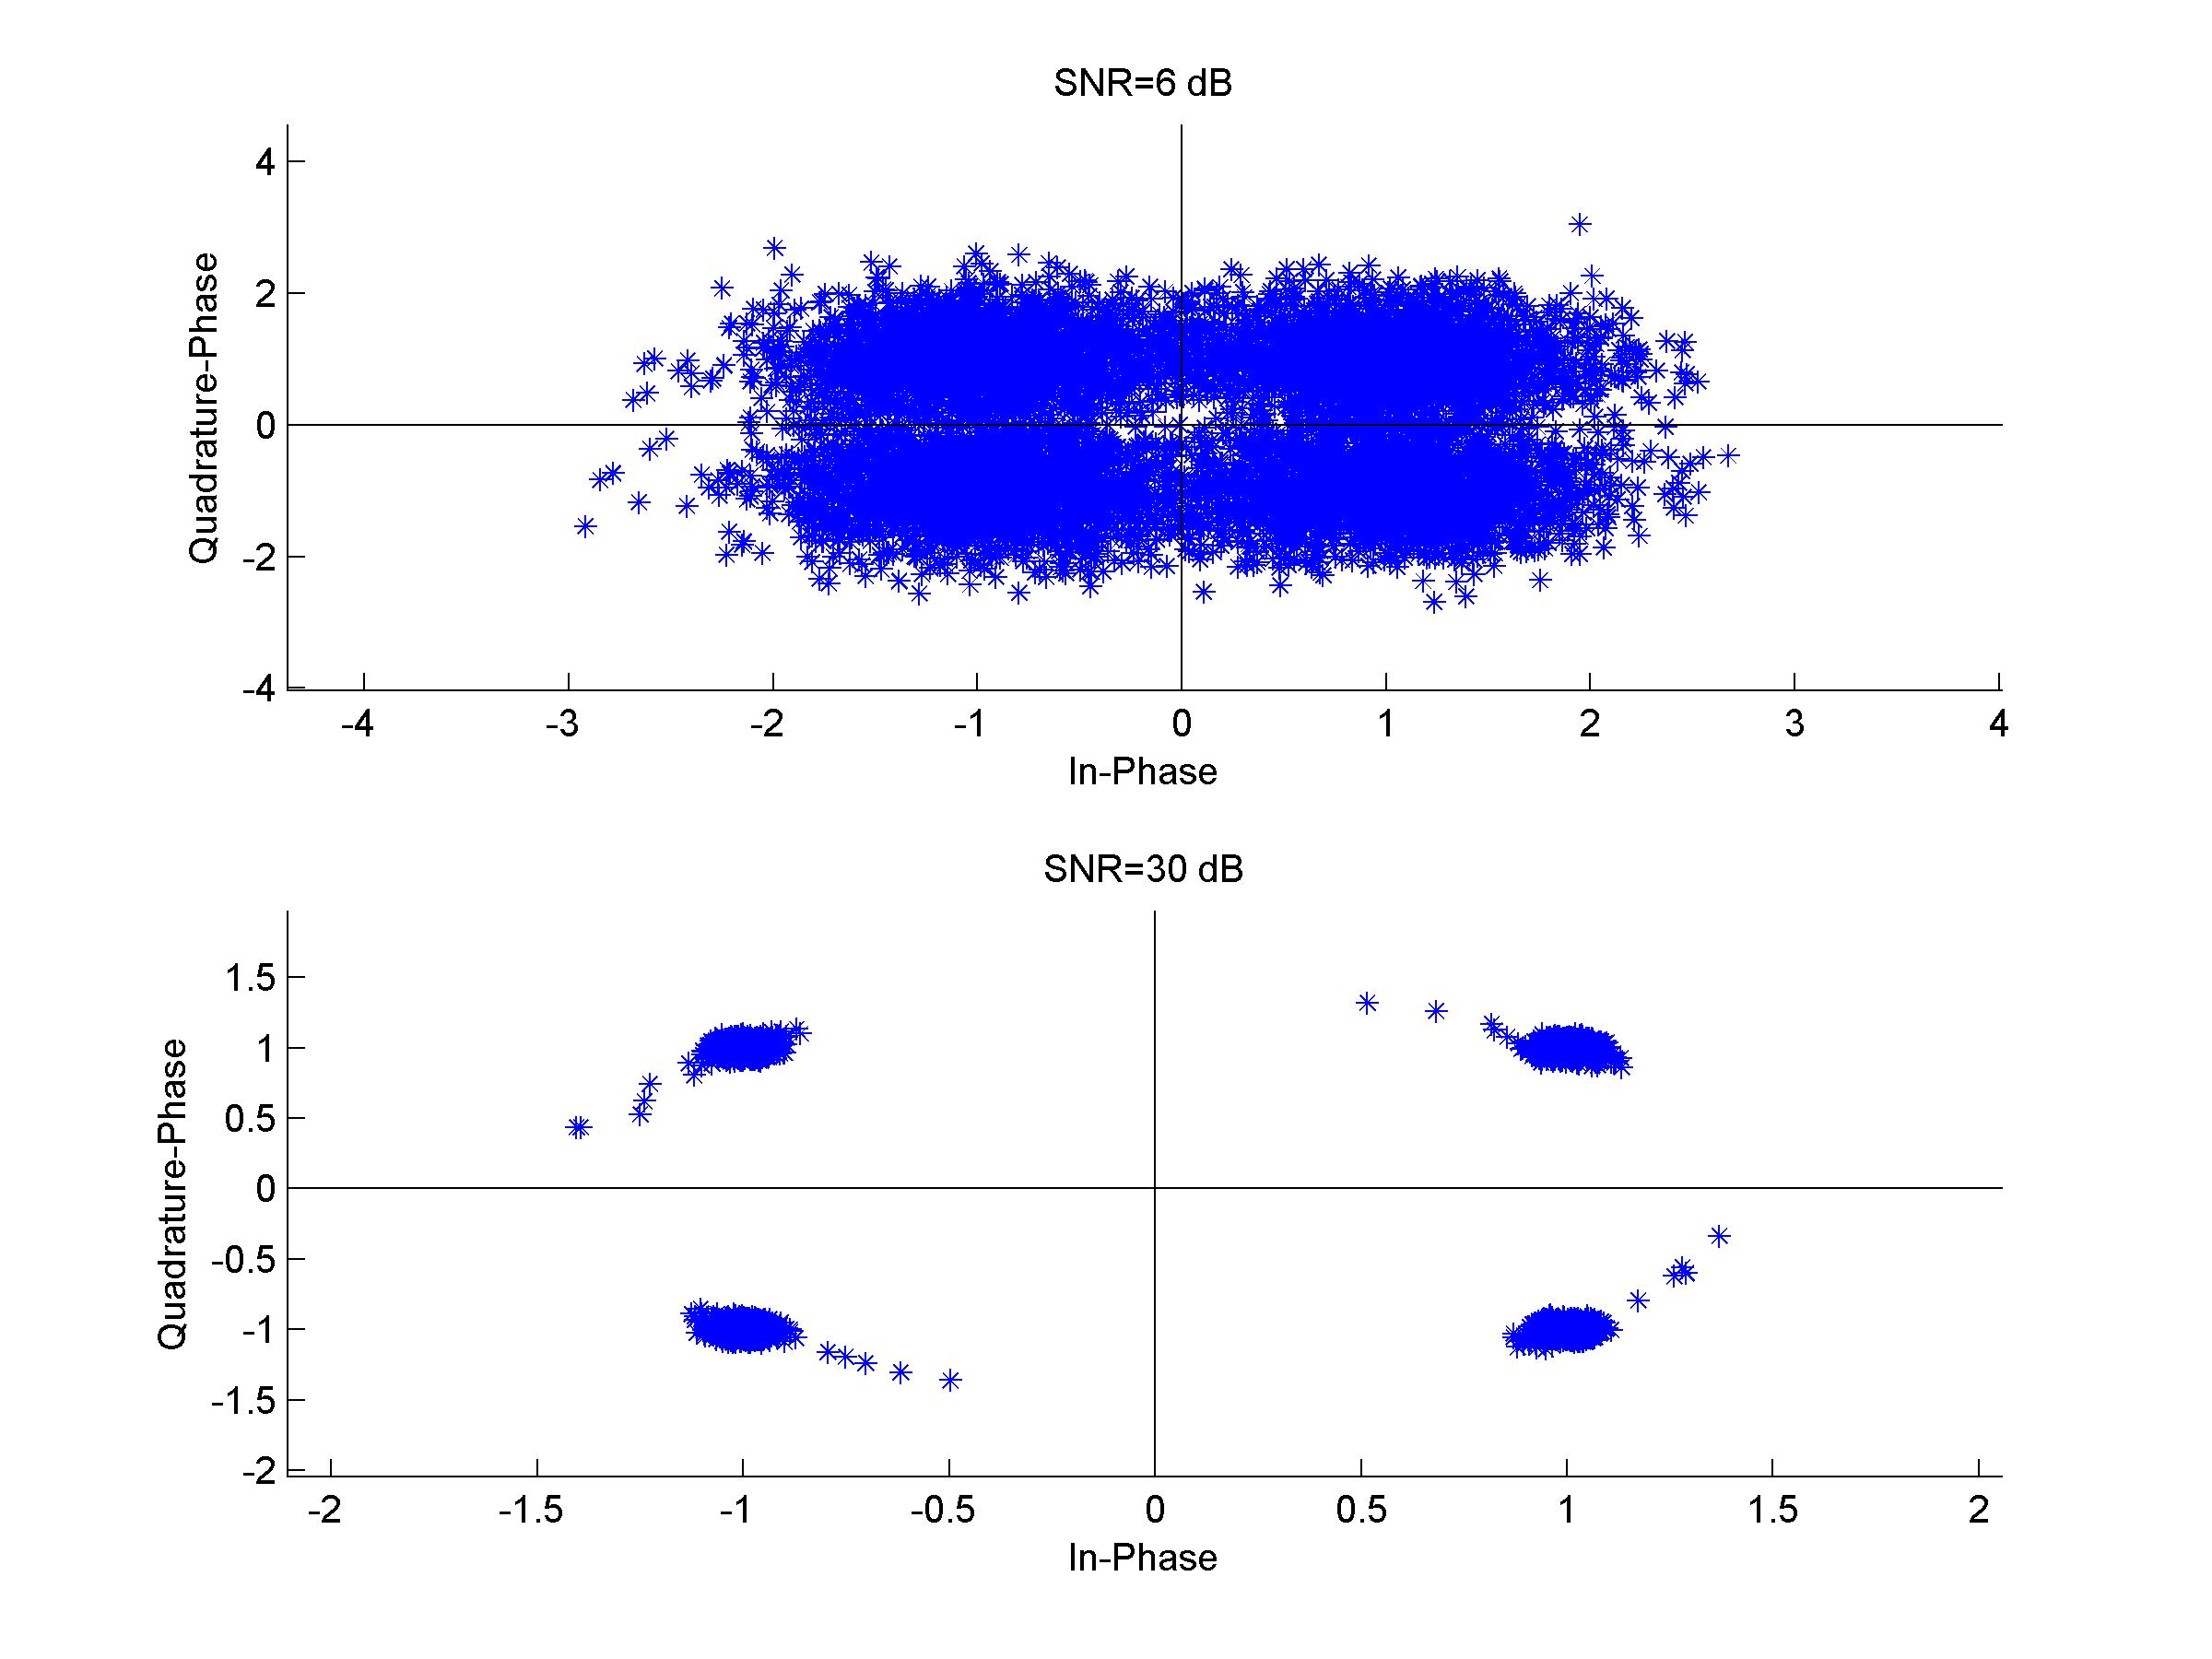
\includegraphics[width=0.7\textwidth]{qpConstpo_ddr1.jpg}
\caption{The resulting constellation plot of the output of the system with Decision Directed Recovery Loop for an input with 30 degrees phase offset at 6dB and 30dB SNR }
\end{figure}

\subsubsection{Constellation Plots  for Frequency Recovery}
\begin{figure}[H]
\centering
\hspace*{-2cm}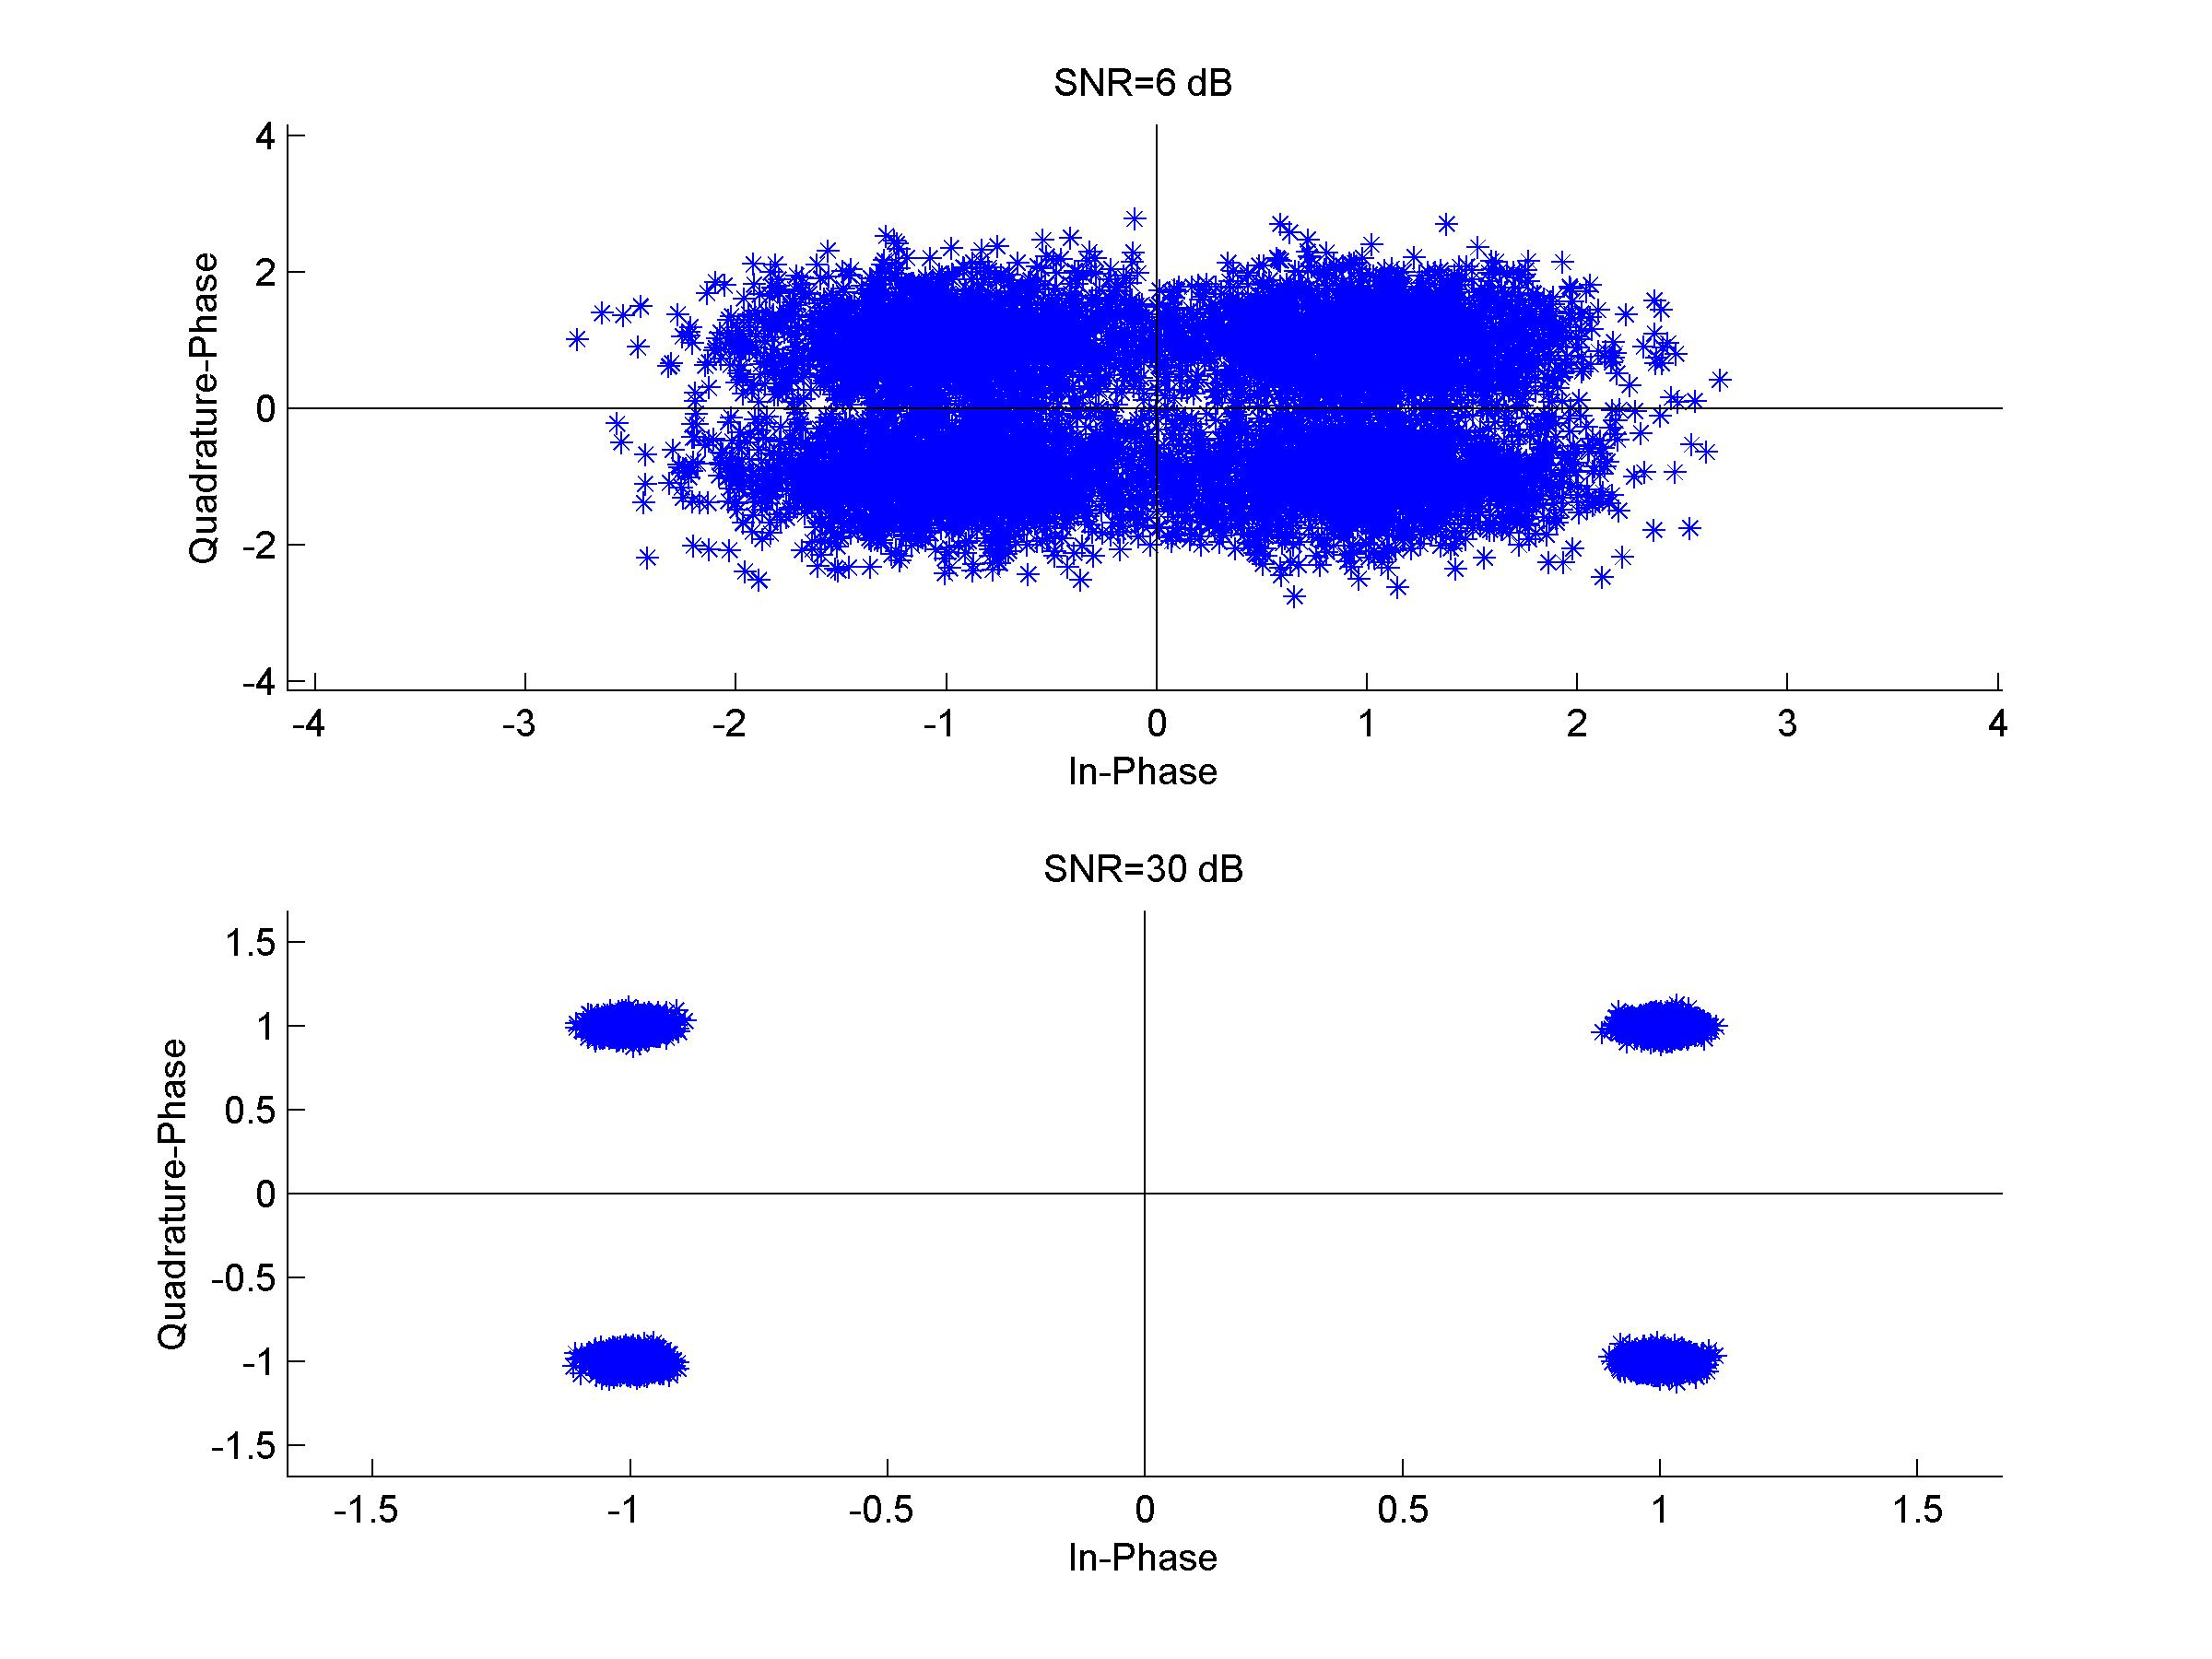
\includegraphics[width=0.7\textwidth]{qpConstfo_ddr1.jpg}
\caption{The resulting constellation plot of the output of the system with Decision Directed Recovery Loop for an input with 1ppm frequency offset at 6dB and 30dB SNR }
\end{figure}

\begin{figure}[H]
\centering
\hspace*{-2cm}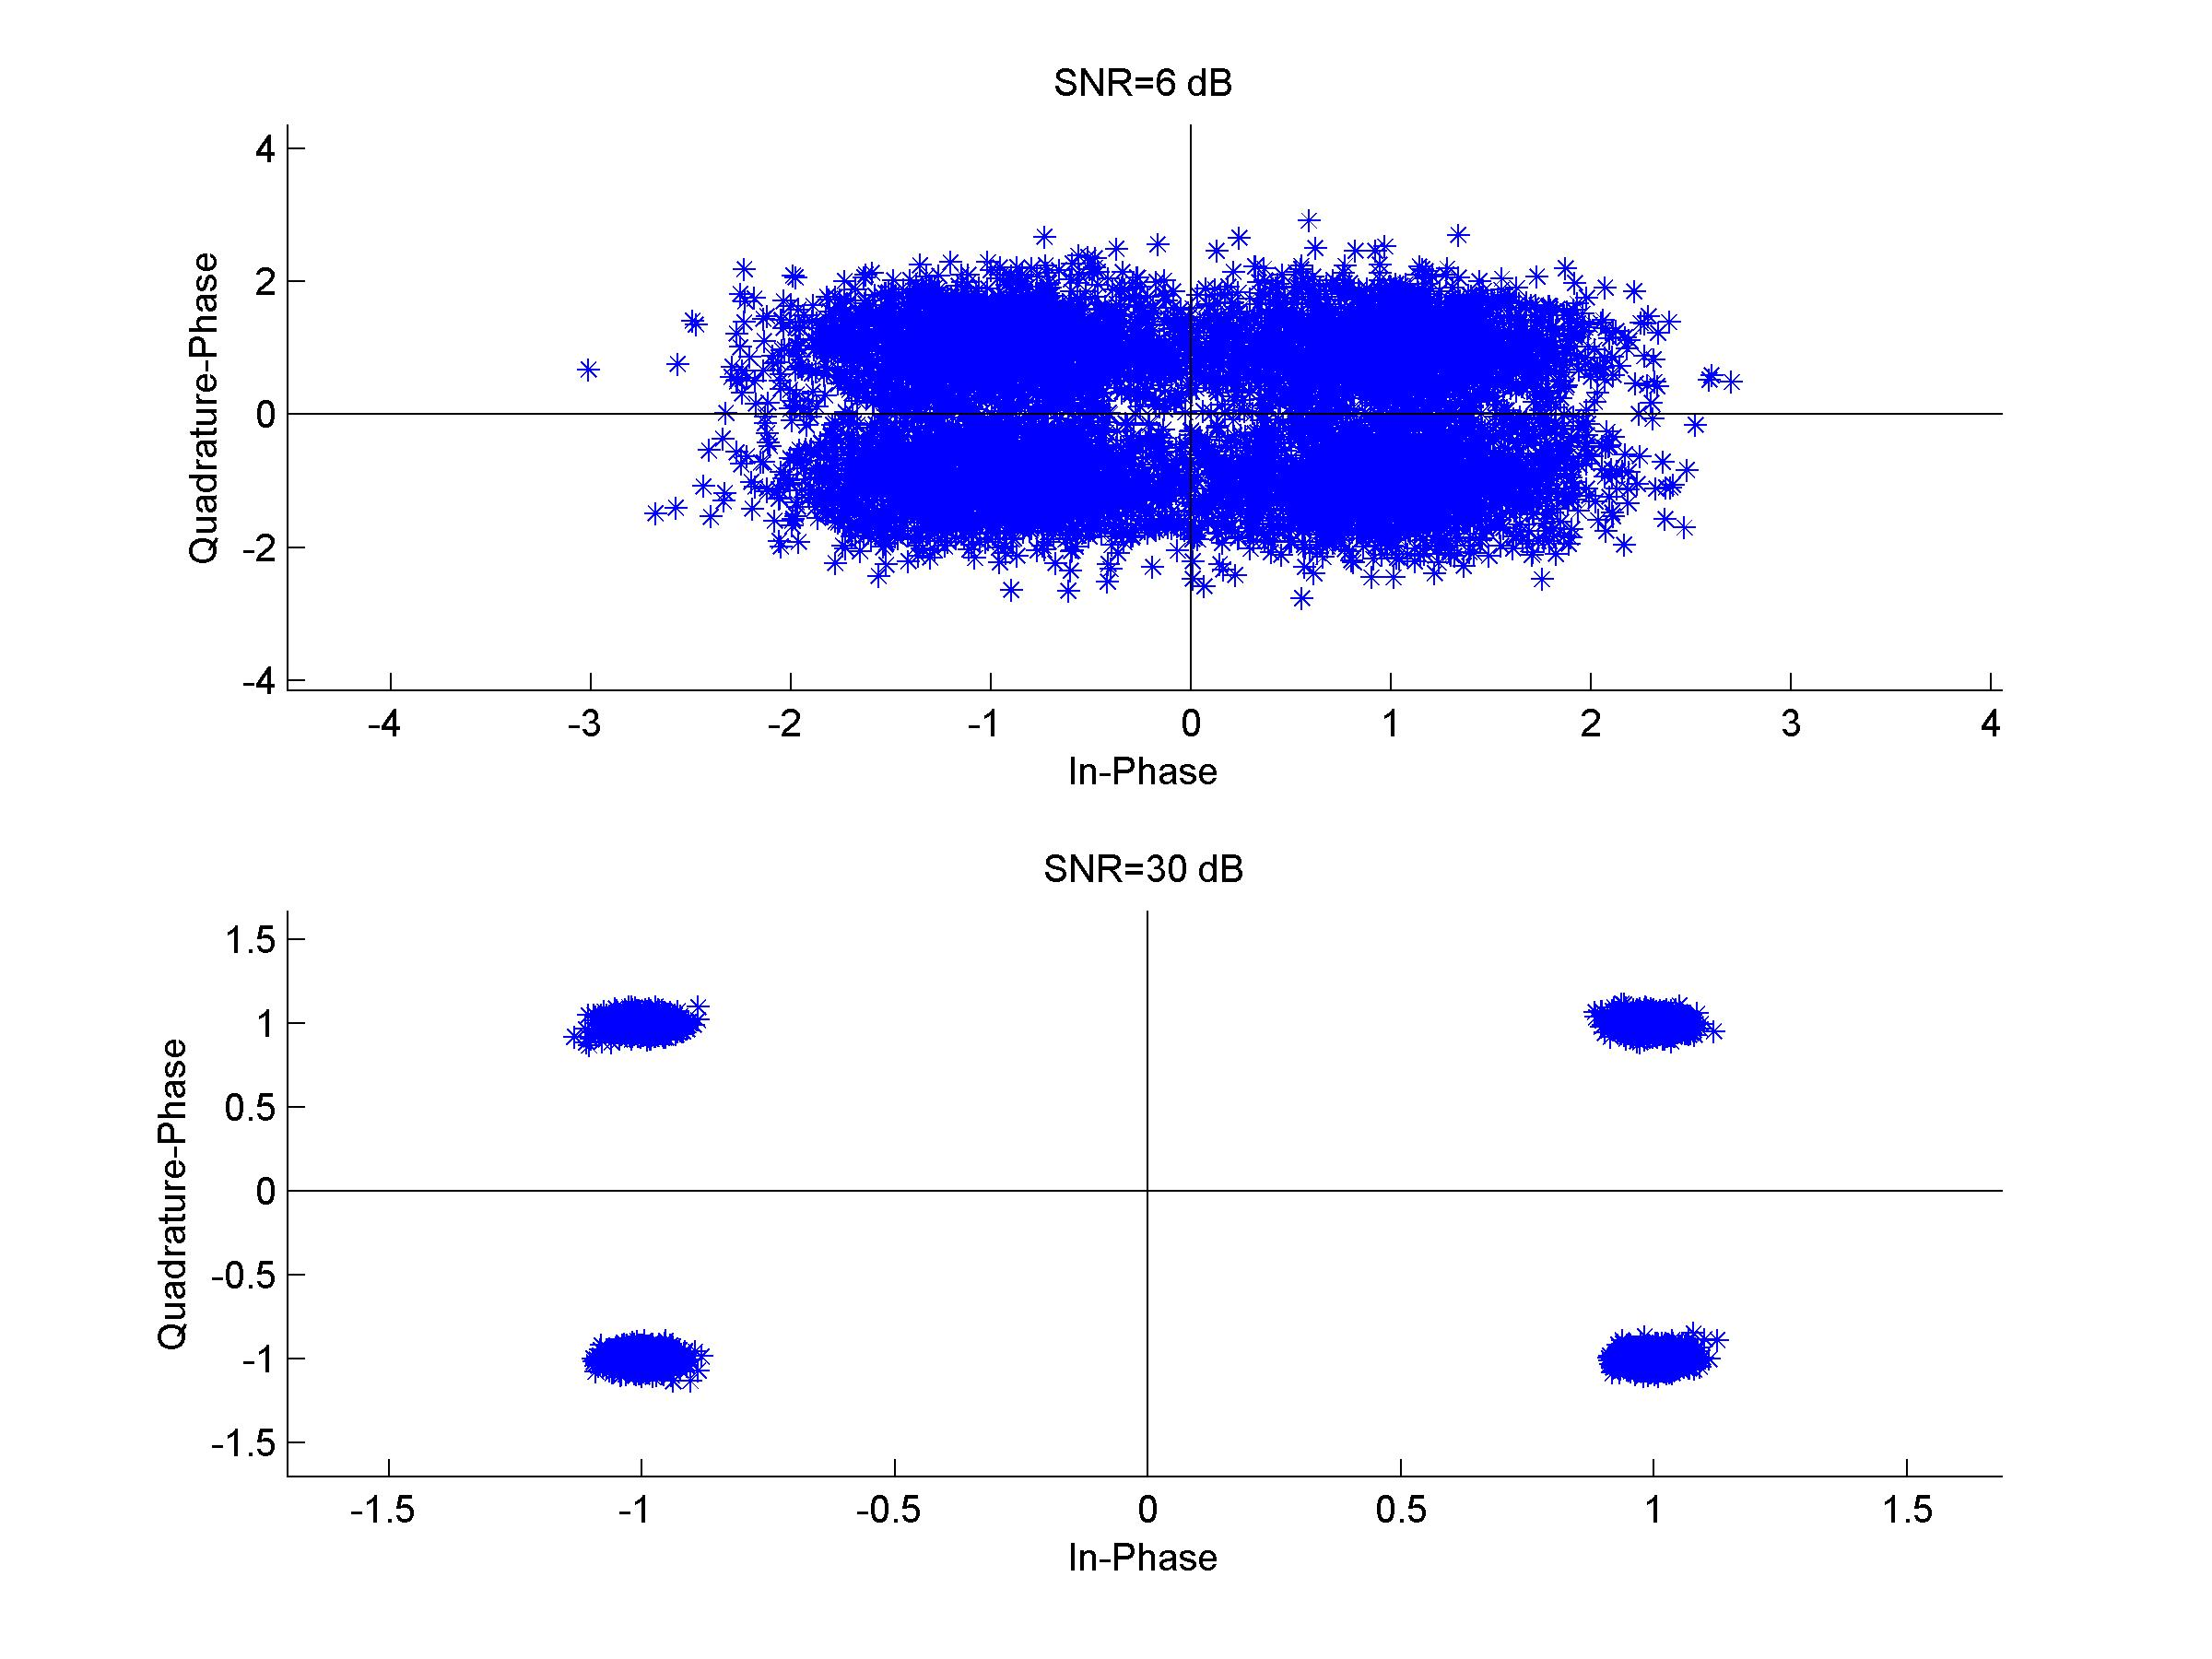
\includegraphics[width=0.7\textwidth]{qpConstfo_ddr2.jpg}
\caption{The resulting constellation plot of the output of the system with Decision Directed Recovery Loop for an input with 30 ppm frequency offset at 6dB and 30dB SNR }
\end{figure}


\subsubsection{BER Plots for Carrier Recovery}
\begin{figure}[H]
\centering
\hspace*{-2cm}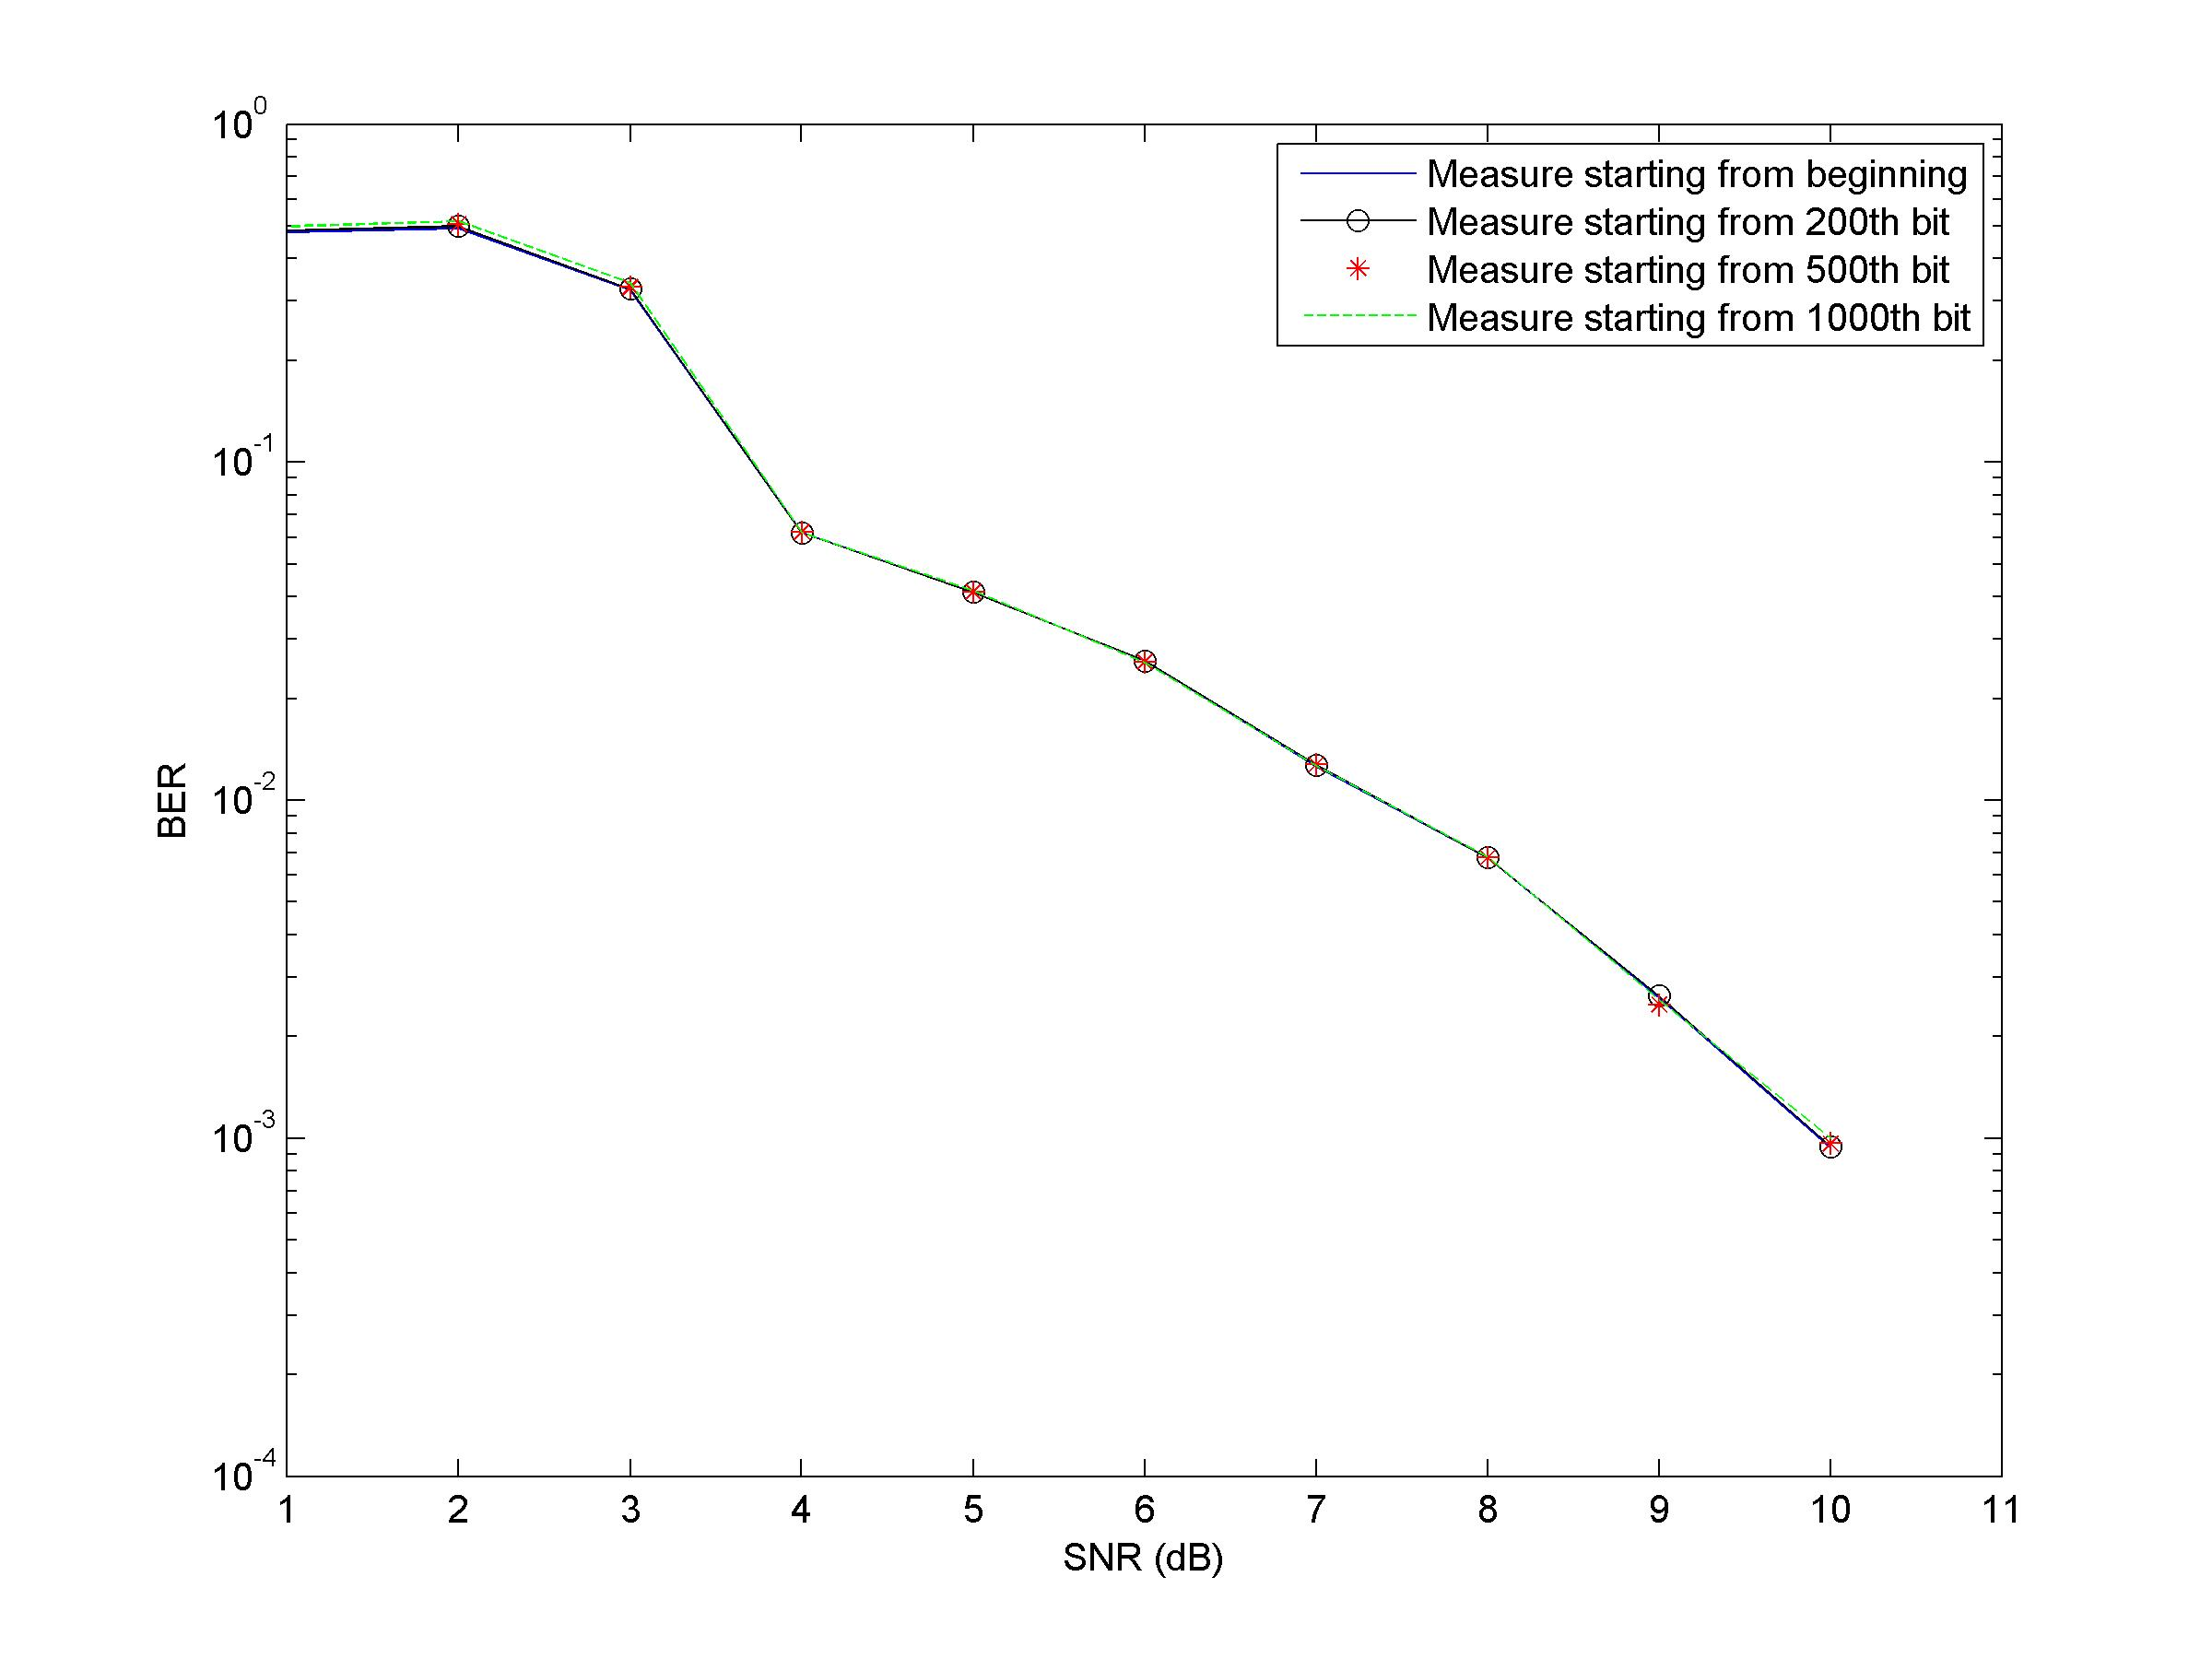
\includegraphics[width=0.7\textwidth]{qpBERfo_ddr1.jpg}
\caption{BER plots of the system with Decision Directed Recovery Loop for an input with 1ppm frequency offset (using output bits starting from different indices)}
\end{figure}

\begin{figure}[H]
\centering
\hspace*{-2cm}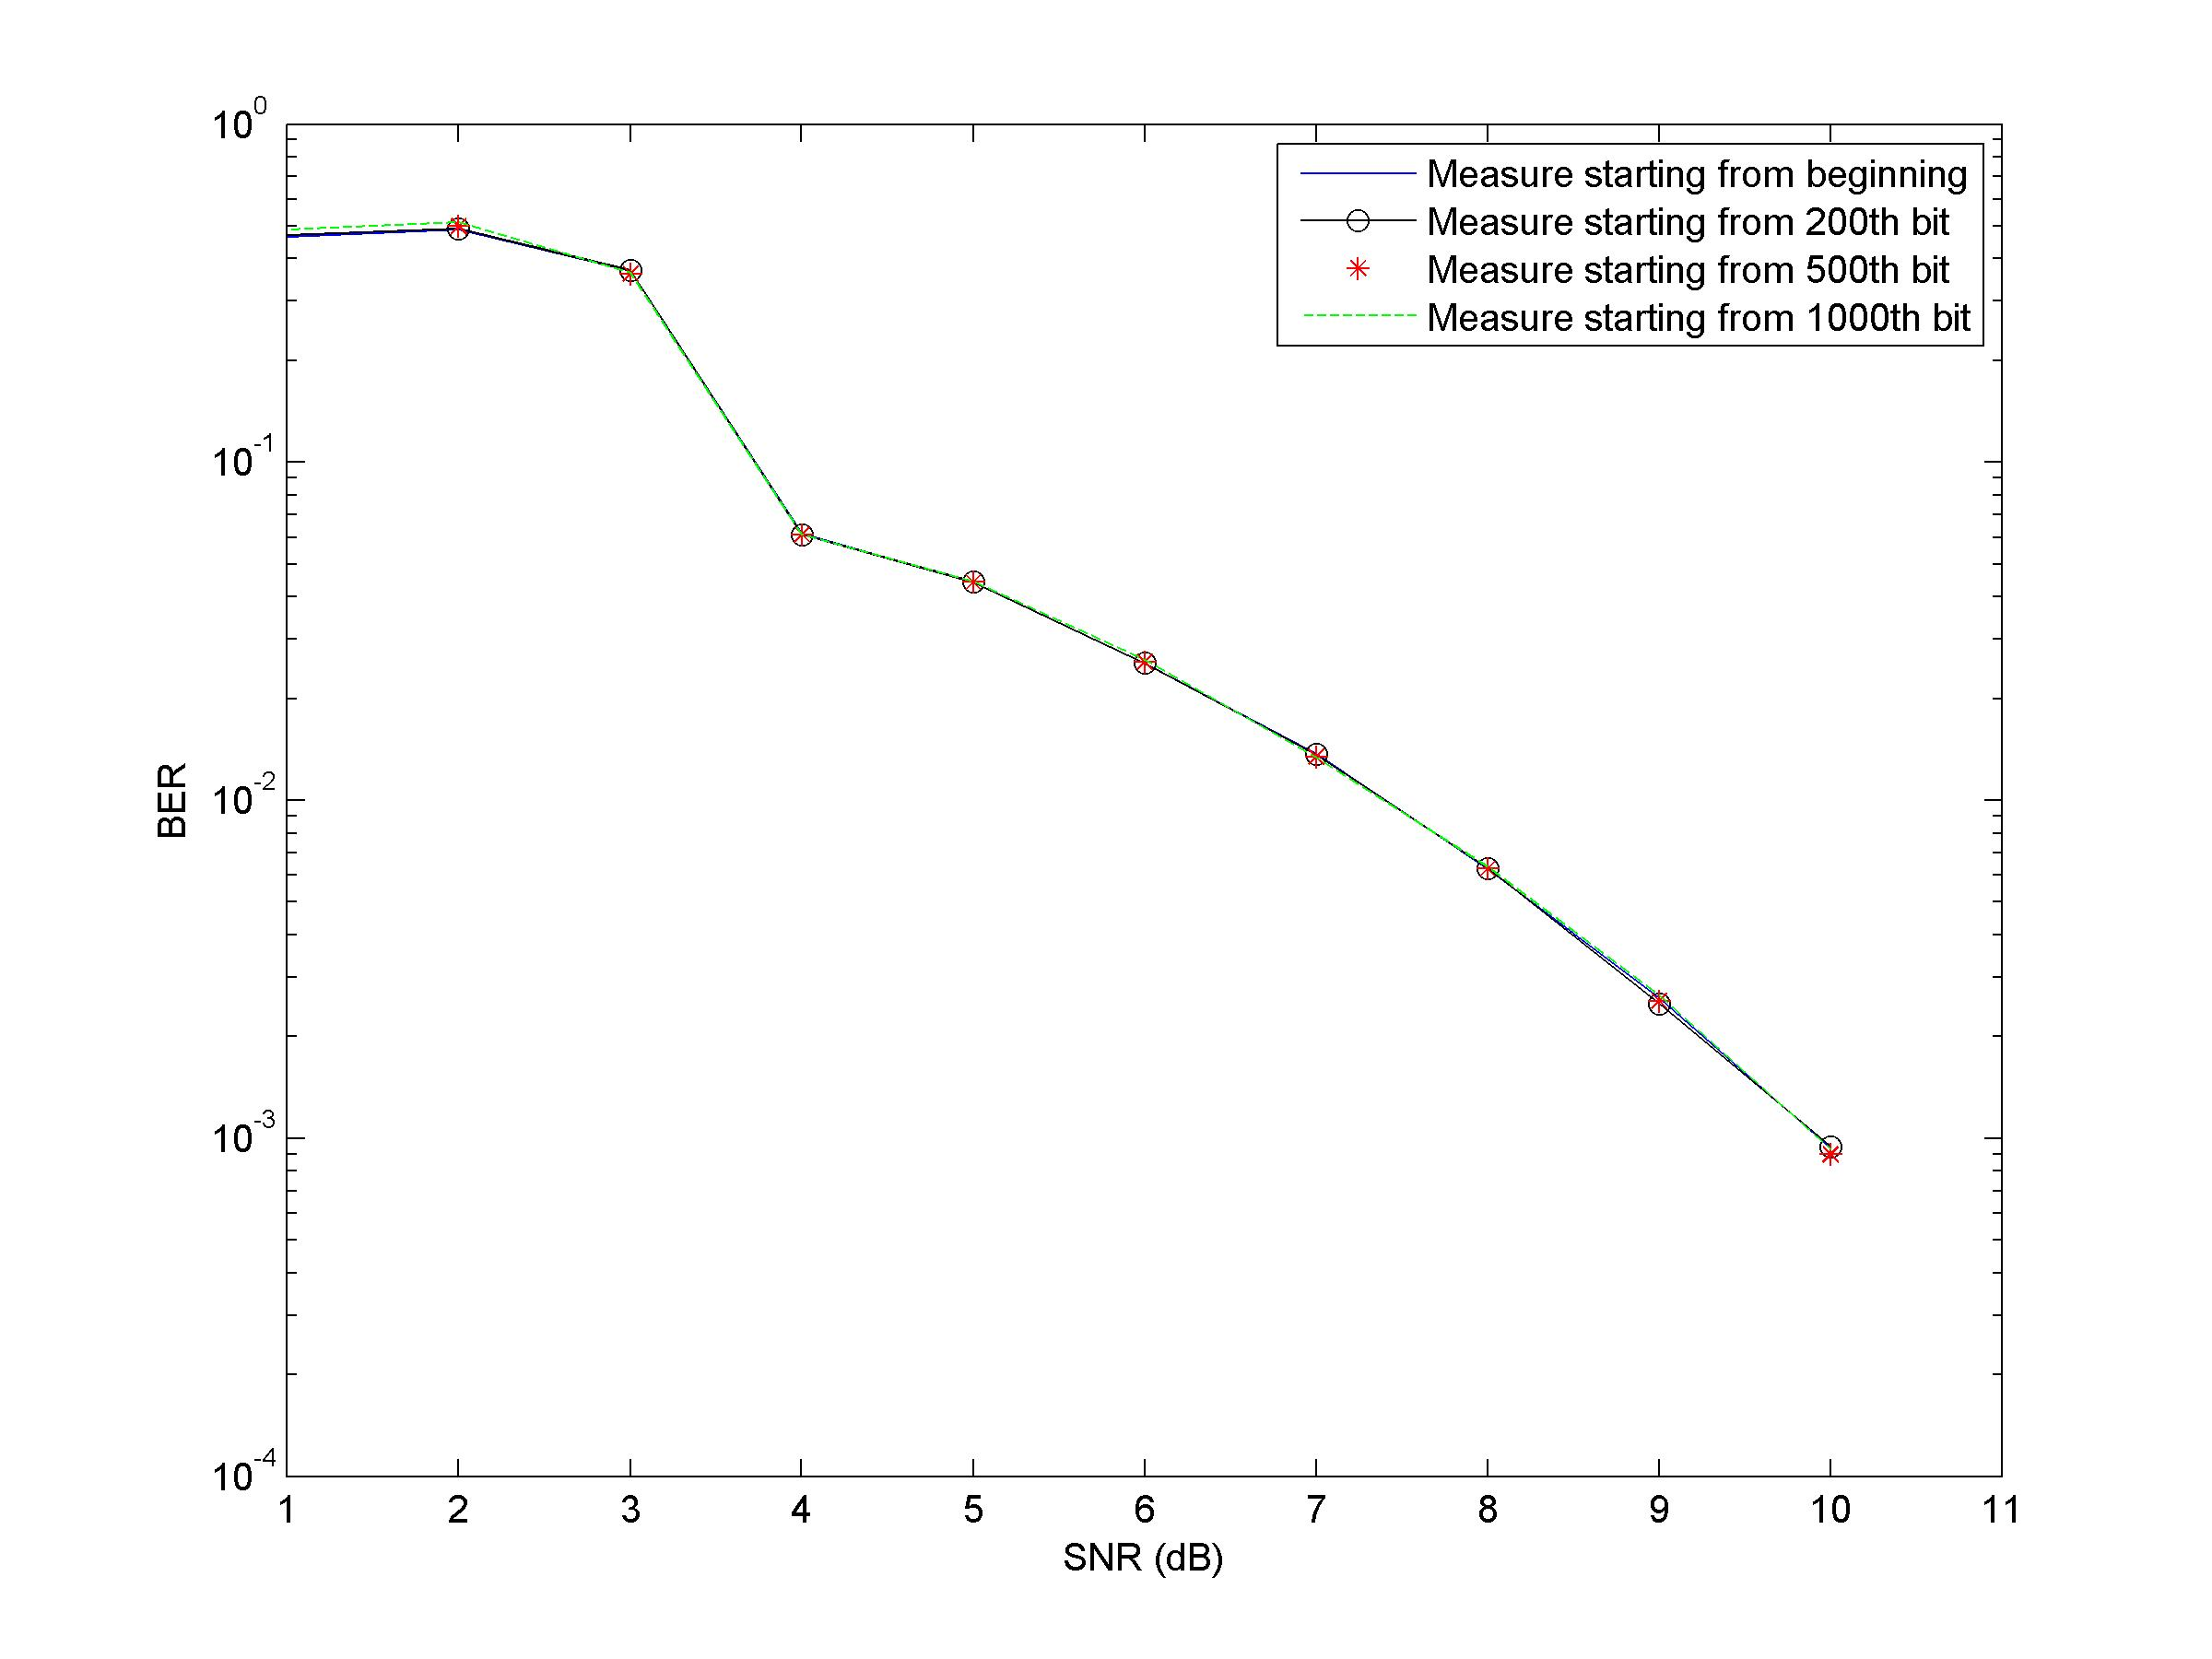
\includegraphics[width=0.7\textwidth]{qpBERfo_ddr2.jpg}
\caption{BER plots of the system with Decision Directed Recovery Loop for an input with 30ppm frequency offset (using output bits starting from different indices)}
\end{figure}

\subsubsection{BER Plots for Phase Recovery}
\begin{figure}[H]
\centering
\hspace*{-2cm}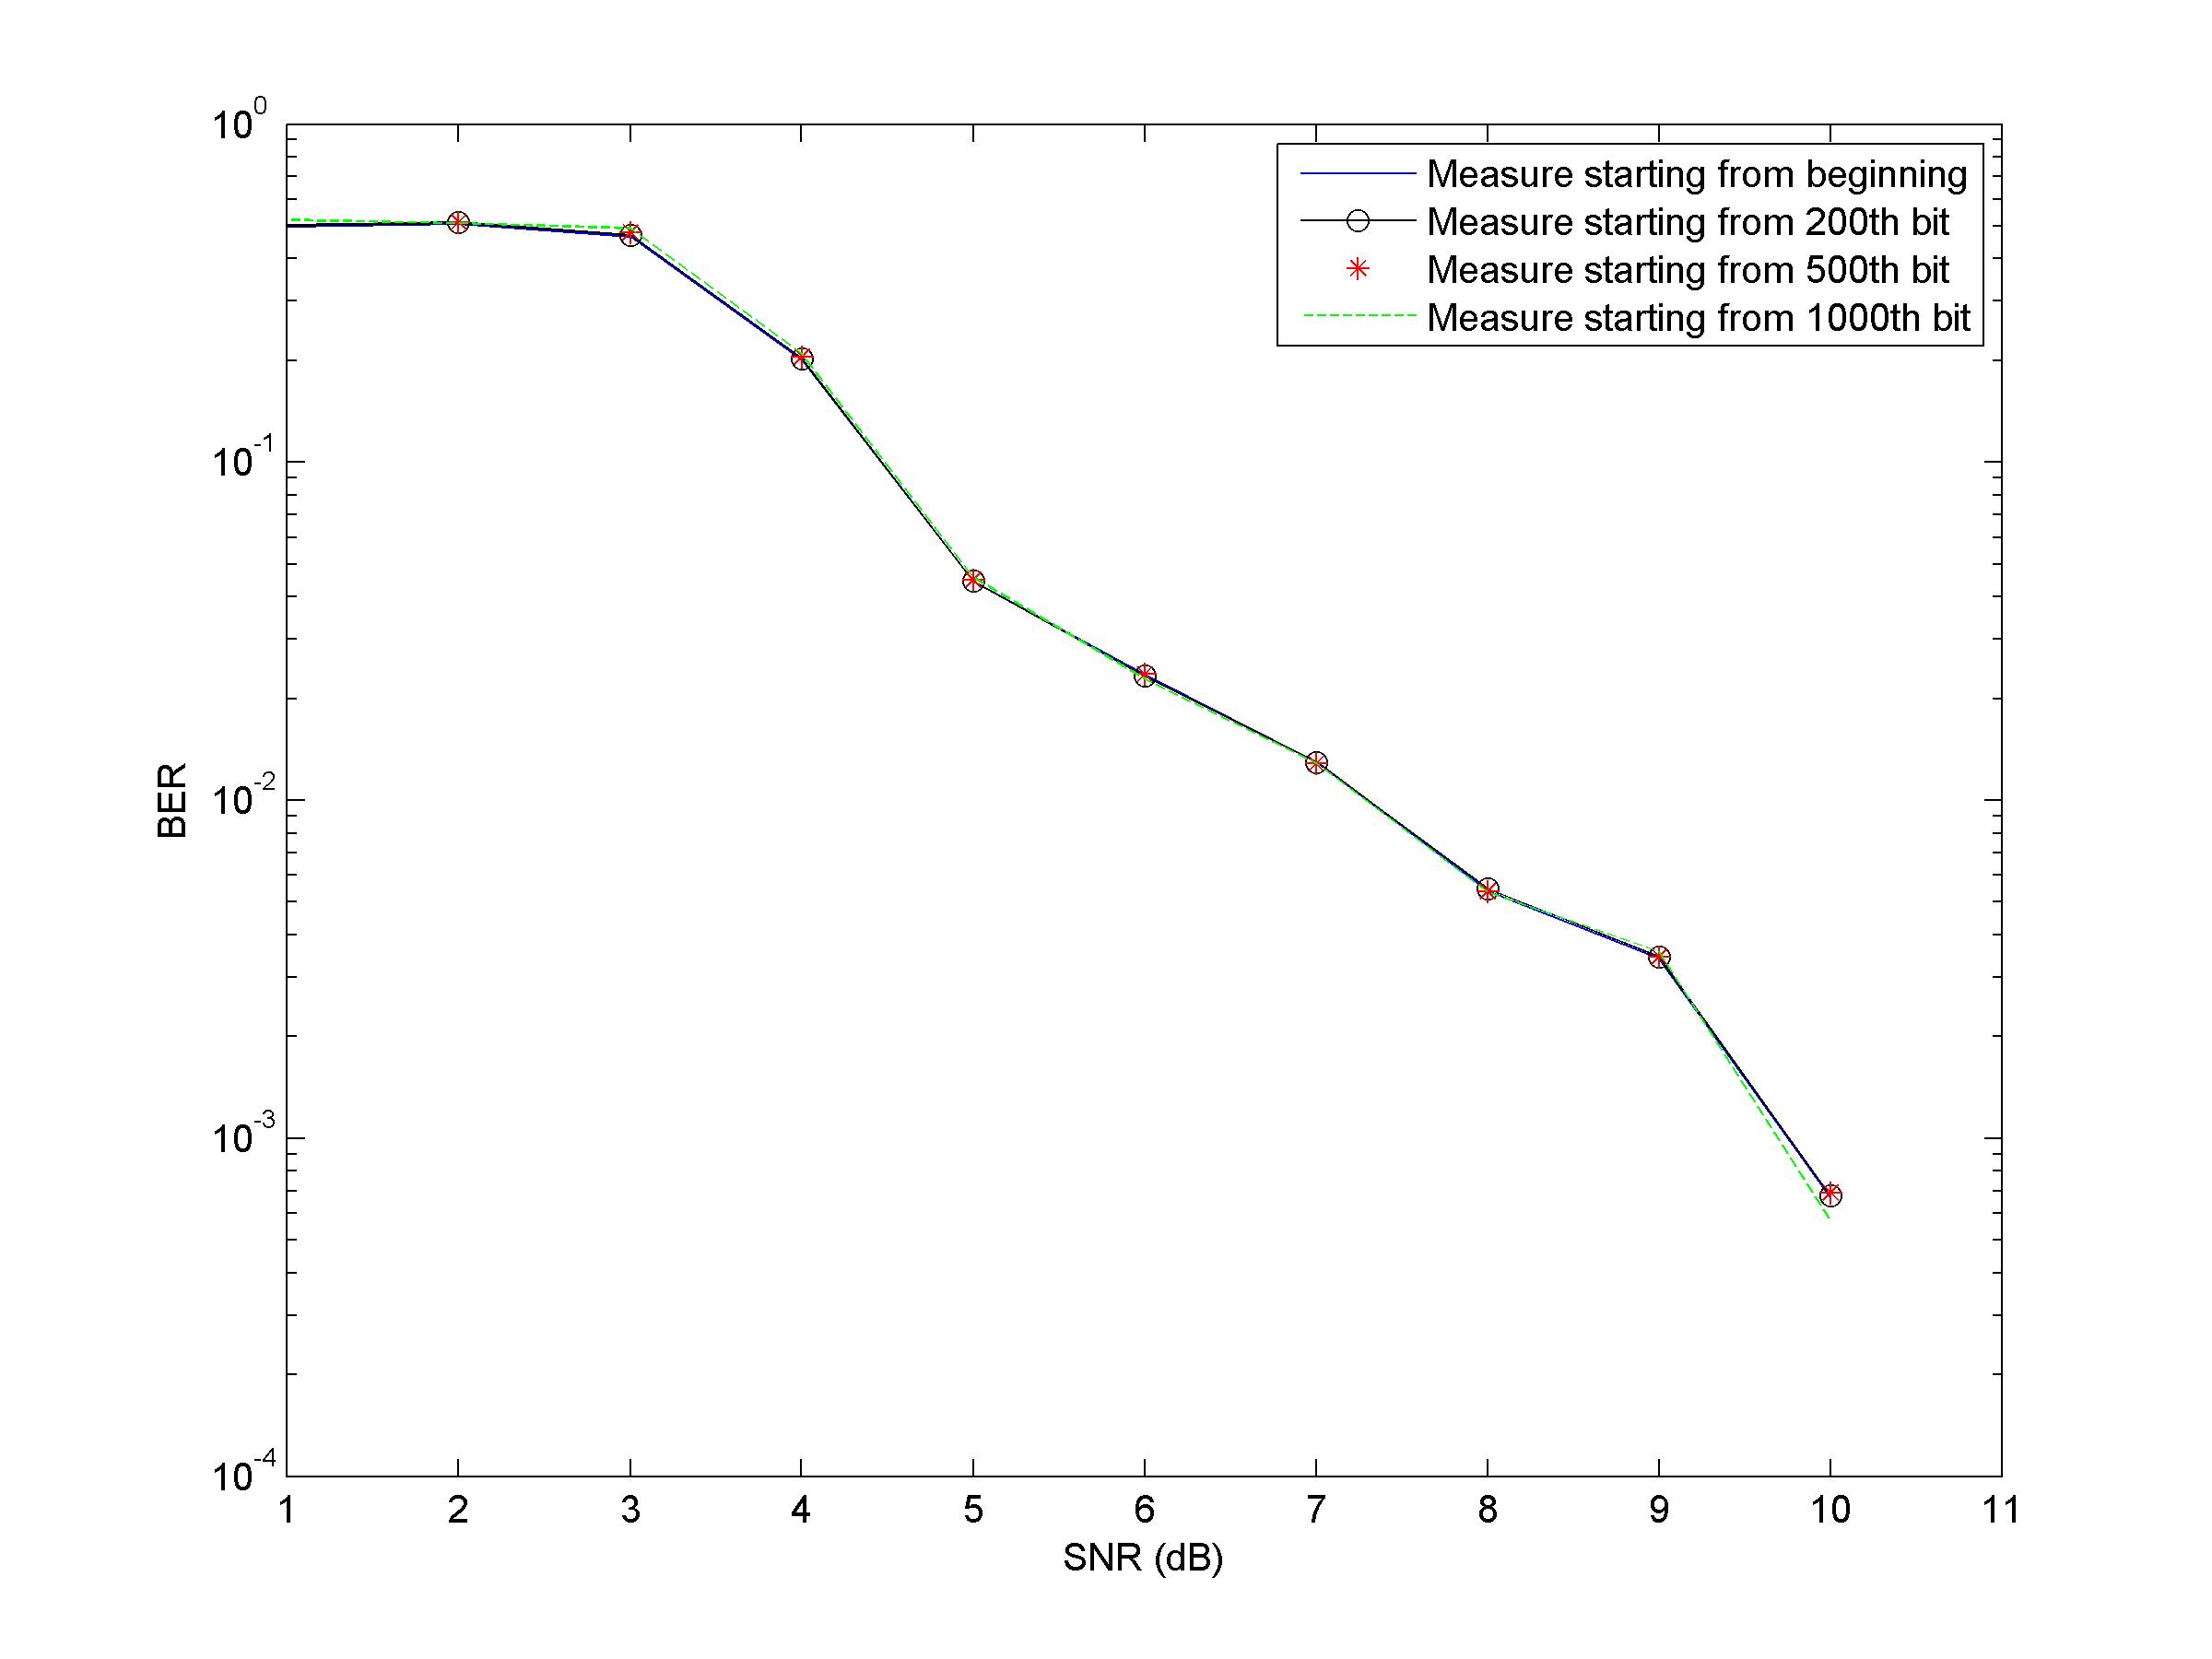
\includegraphics[width=0.7\textwidth]{qpBERpo_ddr1.jpg}
\caption{BER plots of the system with Decision Directed Recovery Loop for an input with 30 degrees phase offset (using output bits starting from different indices)}
\end{figure}

\newpage
\section{Conclusion}
\label{sec:conc}

The objective of this step was to recover the system from the phase and frequency offsets that might be present in the received signal.  To handle the noncoherent error introduced into the system, feedback loops(costas and decision directed) were installed. To combat this, the error is estimated and then fed into a feedback loop filter to track it out. 

-s-curve results
-transience results
-constellation plot results
-where should we start measuring the bits? -> ber results

\appendix
\newpage
\bibliographystyle{plain}
\bibliography{step3}
\newpage
%% the \\ insures the section title is centered below the phrase: Appendix B
%\section{Project Assignment}
%\label{app:assign}
%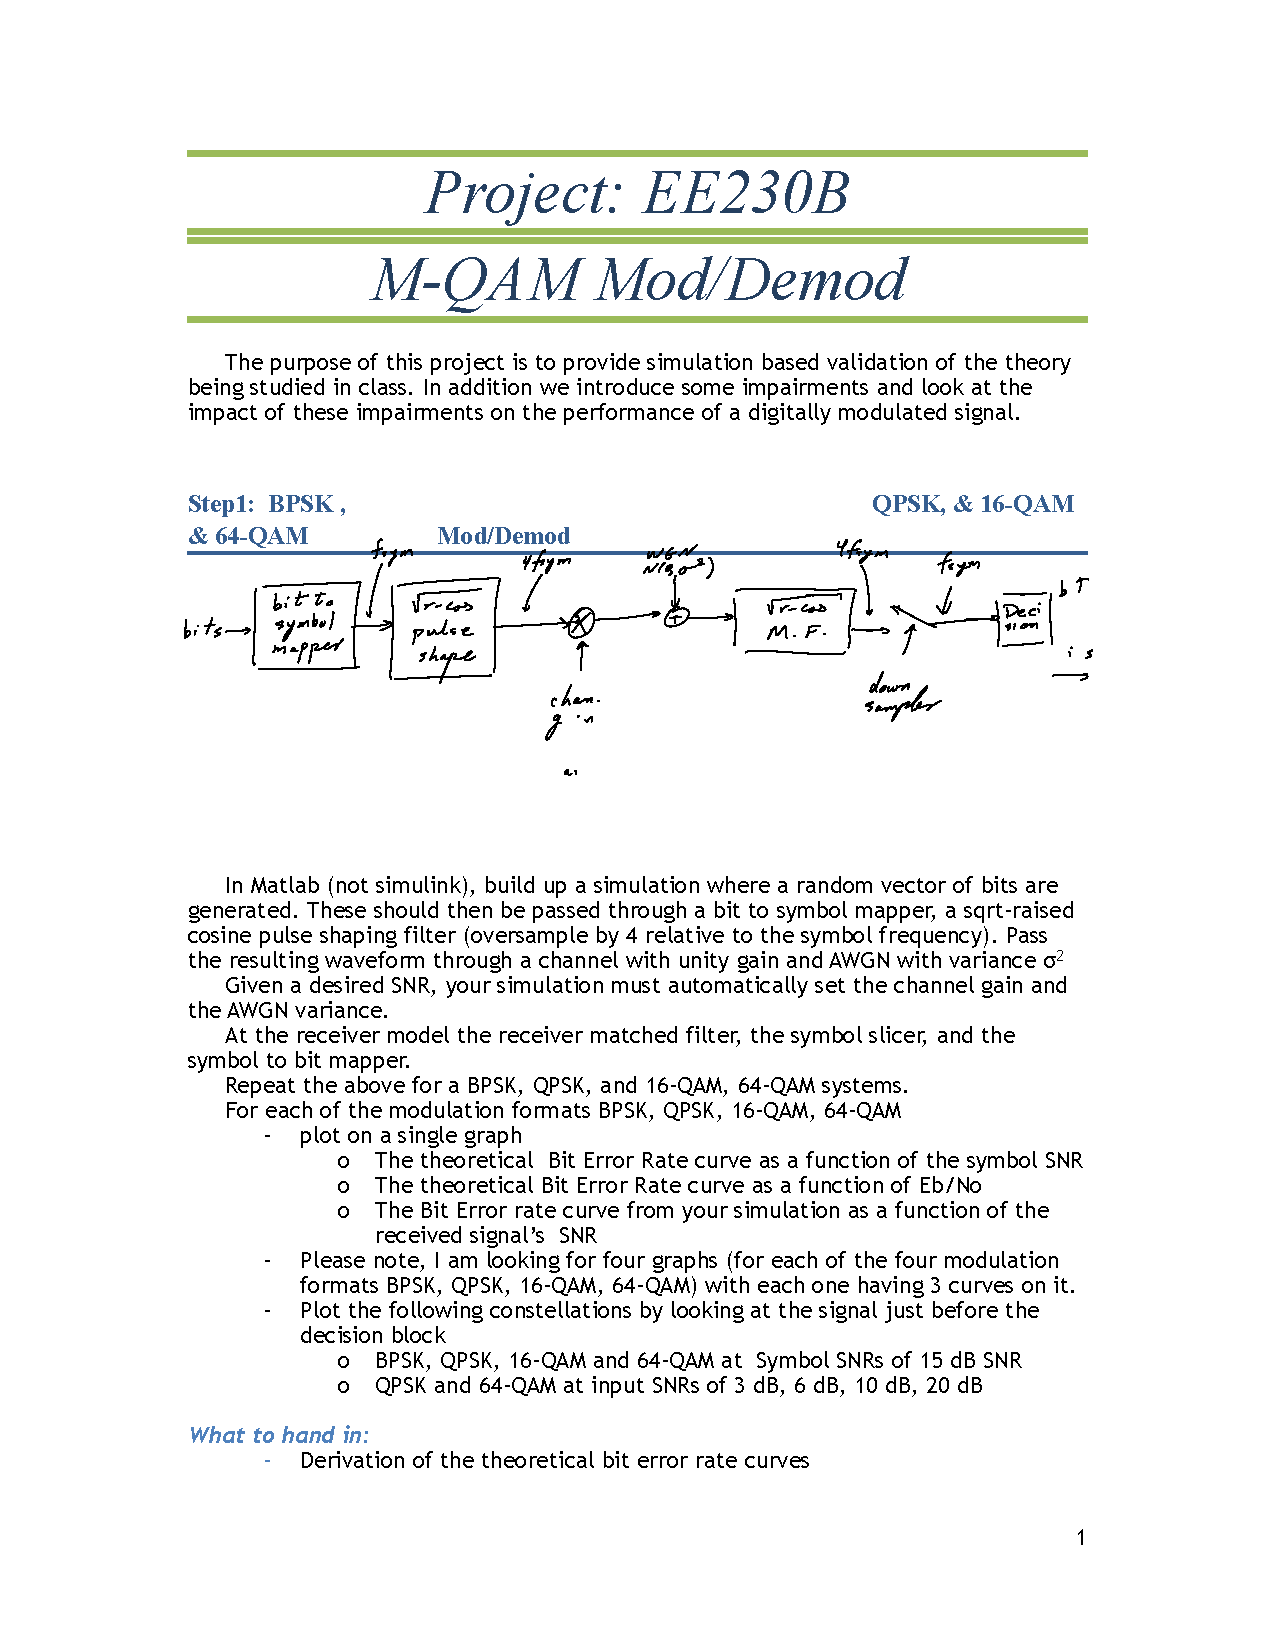
\includepdf[pages={1-5}]{project_overview.pdf}
%\cleardoublepage
%\newpage

\section{Costas Loop}
\subsection{Costas Loop Simulation for Phase Recovery}
\lstinputlisting{step3_costas_phase_qpsk.m}

\subsection{Costas Loop Simulation for Carrier Recovery}
\lstinputlisting{step3_costas_freq_qpsk.m}

\section{Decision Directed Recovery Loop}
\subsection{Decision Directed Recovery Loop Simulation for Phase Recovery}
\lstinputlisting{step3_ddr_phase_qpsk.m}

\subsection{Decision Directed Recovery Loop Simulation for Carrier Recovery}
\lstinputlisting{step3_ddr_freq_qpsk.m}

\section{VCO}
\lstinputlisting{voltage_controlled_osc.m}

\section{Loop Filter}
\lstinputlisting{loop_filter.m}

\section{Random Bit Sequence Generator}
\label{app:random_bit_generator}
\lstinputlisting{random_bit_generator.m}

\section{Bit to Symbol Mapper}
\label{app:bittosym}

\subsection{QPSK Modulation}
\label{app:qpsk_mod}
\lstinputlisting{qpsk_mod.m}

\section{Square Root Raised Cosine Filter}
\label{app:sqrt_raised_cosine}
\lstinputlisting{sqrt_raised_cosine.m}

\section{Up Sampler}
\label{app:impulse_train}
\lstinputlisting{impulse_train.m}

\section{Additive Gaussian White Noise Channel}
\label{app:awgn_channel}
\lstinputlisting{awgn_complex_channel.m}

\section{Sampler}
\label{app:sampler}
\lstinputlisting{sampler.m}

\section{Decision Block}
\label{app:dblocks}
\subsection{QPSK Demodulation}
\label{app:qpsk_demod}
\lstinputlisting{qpsk_demod.m}

\section{Offsets}
\label{app:offsets}
\subsection{Carrier Phase Offset}
\label{app:phase_offset}
\lstinputlisting{phase_offset.m}

\subsection{Carrier Frequency Offset}
\label{app:freq_offset}
\lstinputlisting{freq_offset.m}



\end{document}